%%%%%%%%%%%%%%%%%%%%%%%%%%%%%%%%%%%%%%%%
% Classe do documento
%%%%%%%%%%%%%%%%%%%%%%%%%%%%%%%%%%%%%%%%

% Nós usamos a classe "unb-cic".  Deixe apenas uma das linhas
% abaixo não-comentada, dependendo se você for do bacharelado ou
% da licenciatura.

%\documentclass[bacharelado]{unb-cic}
\documentclass[licenciatura]{unb-cic}


%%%%%%%%%%%%%%%%%%%%%%%%%%%%%%%%%%%%%%%%
% Pacotes importados
%%%%%%%%%%%%%%%%%%%%%%%%%%%%%%%%%%%%%%%%

\usepackage[brazil,american]{babel}
\usepackage[T1]{fontenc}
\usepackage{siunitx}
\usepackage{indentfirst}
\usepackage{natbib}
\usepackage{xcolor,graphicx,url}
\usepackage[utf8]{inputenc}
\usepackage{hyperref}
\usepackage{acronym}
\usepackage{textcomp}
\usepackage{epstopdf}
\usepackage{array}
\usepackage{listings}
\usepackage{color}
\usepackage{multirow}


\usepackage{color}

\definecolor{pblue}{rgb}{0.13,0.13,1}
\definecolor{pgreen}{rgb}{0,0.5,0}
\definecolor{pred}{rgb}{0.9,0,0}
\definecolor{pgrey}{rgb}{0.46,0.45,0.48}

\usepackage{listings}
\lstset{language=Java,
  showspaces=false,
  showtabs=false,
  breaklines=true,
  showstringspaces=false,
  breakatwhitespace=true,
  commentstyle=\color{pgreen},
  keywordstyle=\color{pblue},
  stringstyle=\color{pred},
  basicstyle=\ttfamily\footnotesize,
  moredelim=[il][\textcolor{pgrey}]{$$},
  moredelim=[is][\textcolor{pgrey}]{\%\%}{\%\%}
}

%% \definecolor{mygreen}{rgb}{0,0.6,0}
%% \definecolor{mygray}{rgb}{0.5,0.5,0.5}
%% \definecolor{mymauve}{rgb}{0.58,0,0.82}

%% \lstset{ %
%% 	backgroundcolor=\color{white},   % choose the background color; you must add \usepackage{color} or 
%% 	basicstyle=\footnotesize,        % the size of the fonts that are used for the code
%% 	breakatwhitespace=false,         % sets if automatic breaks should only happen at whitespace
%% 	breaklines=true,                 % sets automatic line breaking
%% 	captionpos=b,                    % sets the caption-position to bottom
%% 	commentstyle=\color{mygreen},    % comment style
%% 	deletekeywords={...},            % if you want to delete keywords from the given language
%% 	escapeinside={\%*}{*)},          % if you want to add LaTeX within your code
%% 	extendedchars=true,              % lets you use non-ASCII characters; for 8-bits encodings only, does not work with UTF-8
%% 	frame=single,	                   % adds a frame around the code
%% 	keepspaces=true,                 % keeps spaces in text, useful for keeping indentation of code (possibly needs columns=flexible)
%% 	keywordstyle=\color{blue},       % keyword style
%% 	language=Java,                   % the language of the code
%% 	otherkeywords={*,...},            % if you want to add more keywords to the set
%% 	numbers=left,                    % where to put the line-numbers; possible values are (none, left, right)
%% 	numbersep=5pt,                   % how far the line-numbers are from the code
%% 	numberstyle=\tiny\color{black}, % the style that is used for the line-numbers
%% 	rulecolor=\color{black},         % if not set, the frame-color may be changed on line-breaks within not-black text (e.g. comments (green here))
%% 	showspaces=false,                % show spaces everywhere adding particular underscores; it overrides 'showstringspaces'
%% 	showstringspaces=false,          % underline spaces within strings only
%% 	showtabs=false,                  % show tabs within strings adding particular underscores
%% 	stepnumber=1,                    % the step between two line-numbers. If it's 1, each line will be numbered
%% 	stringstyle=\color{mymauve},     % string literal style
%% 	tabsize=2,	                   % sets default tabsize to 2 spaces
%% 	title=\lstname                   % show the filename of files included with \lstinputlisting; also try caption instead of title
%% }


%%%%%%%%%%%%%%%%%%%%%%%%%%%%%%%%%%%%%%%%
% Cores dos links
%%%%%%%%%%%%%%%%%%%%%%%%%%%%%%%%%%%%%%%%

% Veja o arquivos cores.tex se quiser ver que outras cores estão
% pré-definidas.  Utilizando o comando \hypersetup abaixo nós
% evitamos aquelas caixas vermelhas feias em volta dos links.

%%%%%%%%%%%%%%%%%%%%%%%%%%%%%%%%%%%%%%%%
% Cores do estilo Tango
%%%%%%%%%%%%%%%%%%%%%%%%%%%%%%%%%%%%%%%%

\definecolor{LightButter}{rgb}{0.98,0.91,0.31}
\definecolor{LightOrange}{rgb}{0.98,0.68,0.24}
\definecolor{LightChocolate}{rgb}{0.91,0.72,0.43}
\definecolor{LightChameleon}{rgb}{0.54,0.88,0.20}
\definecolor{LightSkyBlue}{rgb}{0.45,0.62,0.81}
\definecolor{LightPlum}{rgb}{0.68,0.50,0.66}
\definecolor{LightScarletRed}{rgb}{0.93,0.16,0.16}
\definecolor{Butter}{rgb}{0.93,0.86,0.25}
\definecolor{Orange}{rgb}{0.96,0.47,0.00}
\definecolor{Chocolate}{rgb}{0.75,0.49,0.07}
\definecolor{Chameleon}{rgb}{0.45,0.82,0.09}
\definecolor{SkyBlue}{rgb}{0.20,0.39,0.64}
\definecolor{Plum}{rgb}{0.46,0.31,0.48}
\definecolor{ScarletRed}{rgb}{0.80,0.00,0.00}
\definecolor{DarkButter}{rgb}{0.77,0.62,0.00}
\definecolor{DarkOrange}{rgb}{0.80,0.36,0.00}
\definecolor{DarkChocolate}{rgb}{0.56,0.35,0.01}
\definecolor{DarkChameleon}{rgb}{0.30,0.60,0.02}
\definecolor{DarkSkyBlue}{rgb}{0.12,0.29,0.53}
\definecolor{DarkPlum}{rgb}{0.36,0.21,0.40}
\definecolor{DarkScarletRed}{rgb}{0.64,0.00,0.00}
\definecolor{Aluminium1}{rgb}{0.93,0.93,0.92}
\definecolor{Aluminium2}{rgb}{0.82,0.84,0.81}
\definecolor{Aluminium3}{rgb}{0.73,0.74,0.71}
\definecolor{Aluminium4}{rgb}{0.53,0.54,0.52}
\definecolor{Aluminium5}{rgb}{0.33,0.34,0.32}
\definecolor{Aluminium6}{rgb}{0.18,0.20,0.21}

\hypersetup{
  colorlinks=true,
  linkcolor=DarkScarletRed,
  citecolor=DarkScarletRed,
  filecolor=DarkScarletRed,
  urlcolor= DarkScarletRed
}



%%%%%%%%%%%%%%%%%%%%%%%%%%%%%%%%%%%%%%%%
% Informações sobre a monografia
%%%%%%%%%%%%%%%%%%%%%%%%%%%%%%%%%%%%%%%%

\title{Análise estática para detectar a evoulução da linguagem java em projetos open source}

\orientador{\prof \dr Rodrigo Bonifácio de Almeida}{CIC/UnB}
%\coorientador[a]{\prof[a] \dr[a] Coorientadora}{MAT/UnB}
\coordenador{\prof \dr Pedro Antônio Dourado Rezende}{CIC/UnB}
\diamesano{30}{Junho}{2016}

\membrobanca{\prof \dr Genaina Nunes Rodriges}{CIC/UnB}
\membrobanca{\prof \dr Edson Alves da Costa Júnior}{FE/UnB-Gama}

\autor{Thiago Gomes}{Cavalcanti}
\coautor{Vinícius Correa}{de Almeida}

\CDU{004.4}

\palavraschave{análise estática, evolução, evolução de linguagens de programação linguagens, language design, software engeneering, language evolution, refactoring, java}
\keywords{static analysis, language design, software engeneering, language evolution, refactoring, java}





%%%%%%%%%%%%%%%%%%%%%%%%%%%%%%%%%%%%%%%%
% Texto
%%%%%%%%%%%%%%%%%%%%%%%%%%%%%%%%%%%%%%%%
%\makeglossaries
\begin{document}
  \maketitle
  \pretextual

  \begin{dedicatoria}
	  Dedicamos este trabalho a nossa família e ao departamento de Ciência da Computação da UnB. Que este seja apenas uma idéia inicial e que que futuros alunos possam ajudar a enriquecer ainda mais este projeto para que a Universidade tenha sua própria ferramenta de análise de código e que sirva de modelo para outras Universidade.
  \end{dedicatoria}

  \begin{agradecimentos}
	Com imensa dificuldade de agradecer a tantas pessoas que de certo modo nos ajudaram nessa conquista, hora em momentos calmos hora apreensivos. Em especial a toda nossa família por dar todo suporte necessário para que pudessemos concluir essa etapa em nossas vidas, também aluna Daniela Angellos pelo seu desdobramento e conhecimento para nos ajudar a criar essa ferramenta.\\
Em especial ao professor dr. Rodrigo Bonifácio que nos inseriu nesse imenso mundo da Engenharia de Software, hora apresentando um problemática hora ajundando a resolver barreiras as quais não conseguimos sozinhos.\\
E ainda a UnB por todo seu corpo docente que sem este essa jornada não seria concluida com excelência, em especial aoprofessor dr. Edson Alves da Costa Júnior por se deslocar da UnB-Gama para nos ajudar.\\

  \end{agradecimentos}

  \selectlanguage{brazil}
  \begin{resumo}
	Utilizar linguagem de programação como objeto de pesquisa é uma tarefa desafiadora e complexa quer seja para minerar informações quer seja para refatorar, dada a complexidade de manipulação de uma linguagem de programação. Entretanto existe um segmento da engenharia de \textit{software} que recomenda tratar este modelo de \textit{software} como qualquer outro onde este é denominado \textit{Grammarware}. 

Partindo deste segmento, este trabalho de conclusão manipula código fonte da linguagem Java para detectar construções ultrapassadas. O principal objetivo deste trabalho foi tornar transparente a manipulação da linguagem Java para que fosse um simples \textit{input} como em qualquer outro \textit{software}. E isso mais fácil adotar esta ferramenta para checar se a linguagem em que um software qualquer está sendo desenvolvido utiliza sempre características atuais durante o desenvolvimento.

Desta forma o analisador estático que este trabalho proporcionou é capaz de pesquisar construções específicas da linguagem Java que podem ser facilmente determinadas por qualquer desenvolvedor independente da experiência na manipulação dos artefatos de uma linguagem de programação.

Para a extração dos dados este trabalho teve com principal preocupação desacoplar a extração da análise de código para que os dados minerados possam ser salvos em qualquer estrutura de dado que pode ser desde um simples arquivo~\acs{CSV} até um banco de dados.

%Atualmente encontrar blocos de código específicos tem sido de grande importância para atualizar esse trechos por um mais moderno ou mais eficiênte e assim ter os projetos utilizando sempre o que há de mais recente disponibilizado por cada \textit{feature} das linguagem no caso deste trabalho Java.

%Com isso o principal objetivo deste trabalho é criar um analisador estático com o objetivo de encontrar construções específicas na linguagem Java, contruções que podem ser código ultrapassado ou até mesmo modificações de um \textit{foreach} por uma expressão lambda. Tais contruções após encontradas farão parte de um relatório de saída para que possa ser tomada a decisão se tais contruções serão refatoradas ou não.

%Visando a maior flexibilidade possível na contrução deste analisador, a parte responsável por encontrar código fonte pré-determinado é flexível fazendo com que a qualquer momento que seja necessário possam ser criados novos visitantes sem causar impacto na estrutura do analisador. Os relatórios gerados também são flexíveis e automático podendo a qualquer momento ser modificado a geração de arquivos CSV na saída por um banco de dados caso seja de interesse do desenvolvedor.
  \end{resumo}


  \selectlanguage{american}
  \begin{abstract}
  	This job has objective an analyze the software evolution and know how developers evolved software in accordance with evolution of languages specifically in java .
  \end{abstract}
  
  
  \selectlanguage{brazil}


  \tableofcontents
  \listoffigures
  \listoftables
  
  
  %\newpage
  \addcontentsline{toc}{chapter}{Lista de Abreviaturas}
  \chapter*{Lista de abreviaturas}
  \begin{acronym}
\acro{LOC}{Linhas de Código}%
\acro{AST}{Árvore de sintaxe abstrata}%
\acro{IDE}{Ambiente de Desenvolvimento Integrado}
\acro{JDBC}{Java Database Connectivity}
\acro{JDK}{Java Development Kit}
\acro{AWT}{Abstract Window Toolkit}
\acro{RMI}{Invocação de Método Remoto}
\acro{API}{Aplicações de Programação Interfaces}
\acro{JNI}{Java Native Interface}
\acro{GUI}{Interface Gráfica do Usuário}
\acro{JDT}{}
\acro{RSA}{}
\acro{SQL3}{}
\acro{JSE2}{}
\acro{ACDP}{Java Platform Debugger Architecture}
\acro{JAX-WS}{}
\acro{JAXB}{}
\acro{STAX}{}
\acro{JAXP}{}
\acro{JCP}{Java Community Process}
\acro{JVM}{}
\acro{DSA}{}
\acro{MD5}{}
\acro{RSA}{}


\end{acronym}
  
%  \newpage
 % \addcontentsline{toc}{chapter}{List of Abbreviations}
 % \chapter*{List of Abbreviations}
  

  \textual
 
  \chapter{Introdução}



\section{Contexto}
Uma premissa na Engenharia de Software é a \emph{natureza evolutiva} do software, e, com isso, custos significativos são relacionados com as atividades de manutenção. De forma semelhante, as linguagens de programação evoluem, com o intuito de suprir a demandas atuais e crescente. Geralmente a evolução incorpora benefícios visando aumentar a produtividade e facilitar o desenvolvimento para que com isso obtenha-se aumento na qualidade com um esforço condizente. O que acarreta em grande desafio que é evoluir sistemas existentes por aderir novas caracterísiticas incorporadas em versões atuais da linguagens \cite{Dyer:2013} que o projeto utilize.

Conforme discutido por Overbey e Johnson \cite{Overbey:2009}, características incorporadas raramente são removidas de um programa o que as torna obsoleta e assim acarretando em um maior esforço para a manutenção e uma  sobrecarga na complexidade. Isto gera grande esforço na aprendizagem para novos programadores  que são incorporados nestes projetos o que pode vir a elavar os custos de manutenção. 

Por outro lado, a decisão de não modernizar o código fonte em direção a novas versões da linguagem faz com que a equipe de desenvolvimento alterne entre características atuais e antigas, as quais passam a ser quase um dialeto da linguagem confome explica Overbey e Johnson em \cite{Overbey:2009}, --- o que aumenta o tempo para conceber um projeto e consequentemente gerindo aumento no custo final projeto.

Uma decisão não tão simples é manter uma porção do código congelada, sem evolução, ao longo projeto devido alguma restrição técnica. O que infelizmente acarreta em uma estagnação de todo um sistema pois não somente o projeto é afetado, mas sim toda uma infraestrutura como compiladores, banco de dados e sistema operacional que, se de alguma forma vierem a ser atualizados com esta porção código estagnado, podem ocasionar problemas como uma queda significativa de desempenho ou até mesmo o sistema parar de funcionar. Devido a esses problemas de código não atualizado, com as versões com estruturas mais atuais, a proposta da realização de refatoração através de ferramentas objetivam atacar essas limitações decorrentes de código obsoleto.

\section{Motivação}
A principal motivação para este trabalho foi o artigo \textit{Regrowing a Language} \cite{Overbey:2009} que realiza um comparativo entre FORTRAN e Java  e como características de que eram foram incorporadas em FORTRAN por quase meio século foi mantida compatibilidade entre versões atuais e modernas entretando em após FORTRAN-90 alguma características não eram mais suportadas o que acarretou em quebra de compatibilidade com versões atuais o que obrigou desenvolvedores a mirgra para versão mais atual.
	
\section{Problema}
Com a crescente demanda de produção de software cada vez menos tempo é dedicado para evolução de características de um sofrware o que acarretam em códigos que antigos que raramente são removidos. Em alguns casos a evolução é realizado por esforço individual de algum programador ou quando alguma parte do programa necessita ser retrabalhado. Tendo em vista tal problemátca este trabalho tem o intuito não de forçar evolução de características da linguagem Java mas sim criar um ambiente favorável que facilite identificar contruções ultrapassadas. Características essas que serão elencadas mais adiante.

\section{Objetivo}
O principal objetivo deste trabalho é criar um programa capaz de realizar análise estática em projetos desenvolvidos na linguagem Java para caracterizar uso de construções específicas da linguagem com intuito de compreender a forma típica de utlização destas contruções desde que atendam alguns requisitos que serão detalhados no cápitulo \ref{cap:arquiteruta}.
	
Especificamente para que o objetivo principal seja alcançados foram traçados os seguintes objetivos:

	\begin{itemize}
		\item simplicidade para possibilitar desenvolvedores com pouco conhecimento técnico sejam capazes de criar estruturas que possam pesquisar por construções específicas.
	
	  \item implementar um ambiente de análise estática que recupera informações relacionadas ao uso  de construções da linguagem Java. 
	  
	  \item avaliar o uso de construções nas diferentes versões da linguagem Java, considerando  projetos \textit{open-source}. 
	  
	  \item realizar um \textit{survey} inicial para verificar o porqu\^{e} da não adoção de algumas construções  da linguagem nos projetos. 
	  
	  \item contrastar os resultados das nossas análises com trabalhos de pesquisa recentemente publicados, mas que possivelmente não analisam todas as construções de interesse deste trabalho, em particular 
	  a adoção de construções recentes na linguagem (como Expressões Lambda). 
	  
	  \item criar um software que facilite o uso para desenvolvedores com pouco conhecimento técnico.
	\end{itemize}


\section{Estrutura do Trabalho}

 Este trabalho está organizado da seguinte forma:
	\begin{itemize}
		\item Capítulo 1: faz uma introdução do tema e o problema que diversos softwares possuem, específica a problemática a ser trabalhada, a motivação principara para a elaboração deste documento e por fim os objetivos deste trabalho;
		
		\item Capítulo 2: apresenta uma revisão da literatura sobre os temas relacionados a essa monografia (incluindo técnicas para análise estática de código fonte) para provê a fundamentação teórica necessária ao entendimento deste trabalho;
		
		\item Capítulo 3: descreve a arquitetura da ferramenta que é resultado deste trabalho e a maneira como qualquer programador possa vir a utilizá-lo para pesquisar suas características desde que atendam requisitos mínimos;
		
		\item Capítulo 4: \textbf{(a)} apresenta os resultados da replicação do estudo realizado por Parnin \cite{Parnin:ACM2011}, \textbf{(b)} os resultados de uma investigação empírica, seguindo um estilo de pesquisa típico de mineração em 
		repositórios de software, \textbf{(c}) compreender como os desenvolvedores 
		Java utilizam os recursos da linguagem de programação, \textbf{(d)} identificar 
		oportunidades de melhoria de código usando construções mais 
		recentes da linguagem de programação e \textbf{(e)} por fim apresentação das considerações finais e sugestões para trabalhos futuros. 
	\end{itemize}



	
%\section{Objetivos Específicos}
%	Criar um analisador estático de código para projetos java, com foco em projetos \textit{opensource}, e através deste pesquisar através da infraestrutura de árvores sintáticas \cite{chomsky1956three} e visitors \cite{Gamma:1995:DPE:186897} provida pela biblioteca \textit{JDT} do eclipse e encontrar construções de código ultrapassadas e verificar se novas características veem sendo adotados pelo desenvolvedores ao longo do projeto.
%	

%A base deste trabalho eh o desenvolvimento de um suporte ferramental que auxilie na evolução de um código legado para reduzir o uso de construções~  obsoletas. Essas ferramentas tem como base a sua construção em linguagem {\it Java} com o intuito de tornar o processo de construção mais ágil e posteriormente aberto para o acoplamento de novos módulos. A construção de uma árvore sintática é um passo onde é feito para cada arquivo de código {\it .Java} e posteriormente de todos os arquivos {\it .Java} contidos em qualquer projeto para posterior análise. Este parser implica em listar todos os arquivos Java e gerar uma \acs{AST} para que posteriormente haja um percorrimento usando um visitor  \cite{Gamma:1995:DPE:186897} nos blocos de código contidos nos nós da \acs{AST}  \cite{Dyer:2014:MBA:2568225.2568295} afim de compará-los como estes com a versão atual.
%
%O processo de refatoração \cite{Schaefer:2010:SIR:1932682.1869485} tem como motivação a reestruturação de código, de forma que o código considerado pelo processo, morto,duplicado ou com perca de desempenho não haja código morto, duplicado ou com perca de desempenho em um determinado trecho de código. Esse processo não tem como premissa a atualização do código para novas estruturas de versões da linguagem mais recentes. Essa nova abordagem de refatoração tem com motivação a retirada de código obsoleto, devido a novas abordagens e estruturas das novas versões, e com baixo desempenho de sistemas sem prejuízo na sua engenharia e funcionamento.
%
%Devido a esse tipo de refatoração de código visa a evolução do código para a uma mais recente com estruturas onde não haja perda de desempenho devido a mudança e também a atualização do código legado para estruturas modernas. Tais estruturas antigas com a ação dessa proposta de refatoração, tendem com o tempo a sair das estruturas providas pela linguagem Java como aconteceu com Fortan 90 como visto em Overbey  \cite{Overbey:2009:RLR:1639949.1640127} e essa abordagem tem o intuito de diminuir a quantidade de estruturas antigas que não fazem mais sentido pois novas estruturas realizam as mesmas funções no interpretador da linguagem Java. As modificações propostas pela ferramenta de refatoração não deverão trazer com que perca de desempenho ou aumento da complexidade do código portanto deixando como uma sugestão a alteração do código ou segmento de código para o usuário a adesão das propostas de refatoração ou não.
%
%A \acs{AST} proposta por Chomsky em 1956 \cite{chomsky1956three},  é uma estrutura de dados que representa estruturas de cadeias sintáticas representada por um esqueleto semântico da linguagem em questão. É constituída através de um \textit{framework} do ambiente de desenvolvimento integrado chamado Eclipse onde o nome desse \textit{framework} é chamado de EclispeJDT agir sobre traz métodos implementados pelo próprio \textit{framework} para o percorrer e ações na árvore sintática. A ideia é transformar inicialmente qualquer código fonte java em uma árvore sintática e devido a isso, o mapeamento da arvore já construída que é muito conveniente para inspecionar o código fonte de um arquivo ou de um projeto com vários arquivos em diferentes diretórios. Com isso é possível realizar ou sugerir ao usuário modificações no código fonte através desta árvore construída e isto seria referenciado automaticamente no código fonte.
%
%A proposta é criar ferramentas de análise estática para códigos fonte da linguagem Java para que possa-se apurar projetos pequenos e posteriormente em projetos {\it open-sources} para a verificação da existência de alguma defasagem \cite{dyer2013large} de estruturas entre qualquer versão da linguagem Java que fora concebido para a versão atual e estável na qual a linguagem se encontra. O desenvolvimento das ferramentas será com a versão mais atual da linguagem Java que neste momento é o Java versão 8 para verificar se os softwares desenvolvidos está versão nesta versão e como acompanharam a evolução de décadas de novas versões sem atualização do código por motivo de engenharia outro qualquer.


\section{Metodologia}
    
    A realização deste trabalho envolveu atividades de revisão da literatura, contemplando a leitura de artigos científicos e livros que abordam a adoção de novas características de linguagem de programação, análise estática e estudos empíricos sobre adoção de características ao longo do lançamento das diferentes versões~\cite{Schaefer:ACM2009,Parnin:ACM2011,Overbey:2009,bonifacio:scam2015}. Com isso, foi possível compreender a limitação dos trabalhos existentes e, dessa forma, definir o escopo da investigação. 
    
    Posteriormente, foi necessário buscar uma compreensão sobre como implementar ferramentas de 
    análise estática, e escolher uma plataforma de desenvolvimento apropriada (no caso, a plataforma Eclipse-JDT \cite{EclipseJDT}). Posteriormente, foi iniciada a fase de implementação do analisador estático de forma a atender adequadamente a identificação de características da linguagem Java. Além de um ambiente que seja favorecer a inclusão de classes que realizem a pesquisa de caracetrísticas específicas.   
     
    Finalmente, foi seguida uma estrategia de Mineração em repositórios de software, onde foram feitas as análises da adoção de construções da linguagem Java em projetos \textit{open-source}, de forma similar a outros artigos existentes~\cite{pinto-jss:2015,Schaefer:ACM2009, Schaefer:ACM2010, Overbey:2009}.
     
  % \section{Problema a ser Atacado}

Nos últimos anos sistemas computacionais ganharam cada vez mais espaço no mercado o que acarretou na dedicação de profissionais para manter a qualidade elevada tanto no desenvolvimento como na manutenção destes a fim de proporcionar tanto a multiplataforma quanto que qualquer equipe seja capaz de desenvolvem em qualquer local a qualquer tempo.

Com isso a produção de software tornou-se uma tarefa desafiadora de altíssima complexidade que pode acarretar no aumento da possibilidade de surgimento de problemas. Outro fator de grande relevância é que cada vez mais o bom desempenho do software depende da capacidade e qualificação dos profissionais que compõem a equipe de desenvolvimento. Um desses problemas é manter o desenvolvimento com partes ultrapassadas de uma linguagem o que torna um sistema obsoleto e com a chance de conter {\it bugs} e vulnerabilidades que podem comprometer a segurança de todo o sistema.


A atuação de equipes que desenvolvem utilizando códigos obsoletos continua sendo um grande problema no desenvolvimento de software ao longo de suas releases, mesmo com a evolução da linguagem. Códigos mais atuais tornam-se cada vez mais necessário pois evitam, corrigem falhas e vulnerabilidades além do mesmo tornar-se mais atual. Tais códigos não evoluem podem ser por falta de suporte da IDE, por falta conhecimento da equipe de desenvolvedora ou pelo simples fato de não possuir uma analisador estático que aborde estas construções lançadas nas novas versões das linguagens, especificamente java.


Após toda release uma linguagem demora um certo tempo de maturação para que comunidade de desenvolvedores adote novas características lançadas ou simplesmente não a utilizem, porém java possui uma filosofia de manter suporte a todos legado já desenvolvido por questão de portabilidade o que beneficia tanto IDE's quanto equipes a não ter a necessidade de se atualizarem para as ultimas versões da linguagem o que torna a construção de software com uma linguagem ultrapassada confortável porém existe a possibilidade do software possuir vulnerabilidades.

Um bom exemplo a ser lembrado é FORTRAN quando adicionou orientação objetos em sua na sua versão do ano de 2003 forçando a evoulução de seus compiladores os quais não forneciam mais suporte a versões anteriores conforme relata Jeffrey L. Overbey e Ralph E. Johnson em  \cite{Overbey:2009}, que como consequência forçou toda comunidade desenvolvedora a se atualizar. E ainda havia a possiblidade de certos trechos de código sofrer um refectoring em tempo de compilação por um código mais atual e equivalente.

A processo de utilizar um analisador estático em um projeto antes de sua compilação pode vir a impactar na melhora da confiança do software pois pode detectar vulnerabilidades de maneira prematura além de reduzir o retrabalho caso estas não fossem detectadas. Tais vulnerabilidades são falhas que podem vir a ser exploradas por usuários maliciosos, estes podem desde obter acesso ao sistema, manipular dados ou até mesmo tornar todo serviço indisponível. Neste trabalho a criação de um analisador estático terá o intuito de pesquisar trechos de código ultrapassado.

A implementação de {\it refectoring} na grande parte das modernas IDEs mantem suporte para um simples conjunto de código onde o comportamento é intuitivo e fácil de ser analisado,  quando características avançadas de uma linguagem com o java são usados descrever precisamente o comportamento de tarefas é de extrema complexidade além da implementação do refectoring ficar complexa e de difícil entendimento segundo Max Schäfer e Oege de Moor em  \cite{Schaefer:ACM2010}. Modernas IDEs como ecplise realizam complexos refectoring através da técnica de {\it microrefectoring} que nada mais é que a divisão de um bloco de código complexo em pequenas partes para tentar encontrar códigos mais intuitivos a serem modificados.

O analisador estático proposto nesse trabalho tem o objeto de identificar construções ultrapassadas e porções de código congelados que são utilizadas ao logo do desenvolvimento do software verificando o histórico do lançamento das {\it releases} de {\it software} livres desenvolvidos em especialmente usando a linguagem java. Ainda caberá ao desenvolvedor tomar a decisão caso existam construções ultrapassadas nas releases se adotará o {\it refectoring} ou manterá o código congelado expondo o mesmo a usuários maliciosos.

  %\section{História da linguagem}

No começo da decada de 90 um pequeno grupo de engenheros da Oracle chamados de ''Green Team'' acreditava que a próxima onde de na area da computação seria a união de equipamentos eletroeletrônicos com os computadores. O ''Green Team'' liderado por James Gosling, demonstraram que a linguagem de programaçao Java, que foi desenvolvida pela equipe e originalmente era chamado de Oak, foi desenvolvida para dispositivos de entretenimento como aparelhos de tv a cabo, porem não foi bem aceita no meio. Em 1995 com a massificação da Internet, a linguagem Java teve sua primeira grande aplicação o navegador Netscape.

Java é uma linguagem de programação de propósito geral orientada a objetos, concebida especificadademente para ter poucas dependencias de implementação que isso acarreta que uma vez que a aplicação fora desenvolvida ela poderá ser executada em qualquer ambiente computacional.

Na sua primeira versão chamada de Java 1 (\acs{JDK} 1.0.2) haviam oito pacotes básicos do java como: java.lang, java.io, java.util, java.net, java.awt, java.awt.image, java.awt.peer e java.applet. Foi usado para o desenvolvimento de ferramentas populares na epoca como o Netscape 3.0 e o Internet Explorer 3.0.

Sua segunda versão foi o \acs{JDK}1.1 \cite{JDK1.1} que trouxe ganhos em funcionalidades, desempenho e qualidade. Novas aplicações tambem surgiram como : JavaBeans, aprimoramento do \acs{AWT}, novas funcionalidades como o \acs{JDBC}, acesso remoto ao objeto \acs{RMI} e suporte ao padrão Unicode 2.0.

A terceira versão Java 2 (\acs{JDK} 1.2) ofereceu melhorias significativas no desempenho, um novo modelo de segurança, flexível e um conjunto completo de aplicações de programação interfaces \acs{API}'s. Os novos recursos da plataforma Java 2 incluiram: 
\begin{itemize}
  \item O modelo de "sandbox"  foi ampliado para dar aos desenvolvedores, usuários e administradores de sistema a opção de especificar e gerenciar um conjunto de políticas de segurança flexíveis que governam as ações de uma aplicação ou applet que pode ou não ser executada.
  \item Suporte nativo a thread para o ambiente operacional Solaris. Compressão de memória para classes carregadas. Alocação de memória com mais desempenho e melhor para a coleta de lixo. Arquitetura de máquina virtual conectável para outras máquinas virtuais, incluindo a Java HotSpot VMNew. Just in Time (JIT). Java Native Interface \acs{JNI} de conversão.
  \item O conjunto de componentes de projeto, \acs{GUI} (Swing). \acs{API} Java 2D que fornece novos recursos gráficos 2D e \acs{AWT}, bem como suporte para impressão. O Java {\it look and fell}. Uma nova API de acessibilidade.
  \item Framework de entrada de caracteres (suporte a japonês, chinês e coreano). Complexo de saída usando a \acs{API} do Java 2D para fornecer um {\it display} bi-direcional, de alta qualidade de japonês, árabe, hebraico e outras línguas de caracteres.
  \item Java Plug-in para navegadores da web, incluída na plataforma Java 2, fornecendo um tempo de execução totalmente compatível com a máquina virtual Java amplamente implantadas em navegadores.
  \item Invocação das operações ou serviços de rede remoto. Totalmente compatível com Java ORB e incluído no tempo de execução.
  \item \acs{JDBC} que fornece um acesso mais fácil aos dados para consultas mais flexíveis. Melhor desempenho e estabilidade são promovidos por cursores de rolagem e suporte para SQL3 de tipos.
\end{itemize}

Em 8 de Maio de 2000 foi anunciado o Java 2 versão 1.3 que trouxe ganho de desempenho em relação a primeira versão da JS2E de cerca de 40\%  no tempo de {\it  start-up}. Tambem trouxe novas funcionaliadades como: 

\begin{itemize}
  \item O Java HotSpot VM de cliente e suas bibliotecas atentando ao desempenho ao fazer o J2SE versão 1.3 a {\it realease} o mais rápido até à data.
  \item Novos recursos, como o {\it caching applet} e instalação do pacote opcional Java através da tecnologia Java {\it  Plug-in} para aumentar a velocidade e a flexibilidade com que os {\it applets} e aplicativos baseados na tecnologia Java pode ser implantado. Java {\it  Plug-in} tecnologia é um componente do ambiente de execução Java 2 que permite Java {\it applets} e aplicativos para a execução.
  \item O novo suporte para \acs{RSA} assinatura eletrônica, gerenciamento de confiança dinâmico, certificados X.509, e verificação de arquivos o que significa o aumento das possibilidades que os desenvolvedores tem para proteger dados eletrônicos.
  \item Uma série de novos recursos e ferramentas de desenvolvimento da tecnologia J2SE versão 1.3 que permite o desenvolvimento mais fácil e rápido de aplicações baseadas na tecnologia {\it web} ou Java {\it  standalone} de alto desempenho.
  \item A adição de RMI/IIOP e o JNDI para a versão 1.3, melhora na interoperabilidade J2SE. RMI/IIOP melhora a conectividade com sistemas de {\it  back-end} que suportam CORBA. JNDI fornece acesso aos diretórios que suportam o populares LDAP Lightweight Directory Access Protocol, entre outros.
\end{itemize}

No ano de 2002 no dia 6 de Fevereiro, foi lançado a J2SE versão 1.4. Com a versão 1.4, as empresas puderam usar a tecnologia Java para desenvolver aplicativos de negócios mais exigentes e com menos esforço e em menos tempo. As novas funcionalidades como a nova I/O e suporte a 64 bits. A J2SE se tornou plataforma ideal para a mineração em grande escala de dados, inteligência de negócios, engenharia e científicos. A versão 1.4 forneceu suporte aprimorado para tecnologias padrões da indústria, tais como SSL, LDAP e CORBA a fim de garantir a operacionalidade em plataformas heterogêneas, sistemas e ambientes. Com o apoio embutido para XML, a autenticação avançada, e um conjunto completo de serviços de segurança, está versão forneceu base para padrões de aplicações Web e serviços interoperáveis. O J2SE avançou o desenvolvimento de aplicativos de cliente com novos controles de GUI, acelerou Java 2D, a performance gráfica, internacionalização e localização expandida de apoio, novas opções de implantação e suporte expandido para o até então Windows XP.\\

Com a chegada da \acs{JSE2} versão 1.5 (Java 5.0) em 30 de Setembro de 2004, impulsionou benefícios extensivos para desenvolvedores, incluindo a facilidade de uso, desempenho global e escalabilidade, monitoramento do sistema e gestão e desenvolvimento. O Java 5 foi derivado do trabalho de 15 componentes Java Specification Requests (JSRs) englobando recursos avançados para a linguagem e plataforma. Os líderes da indústria na época que participam no grupo de peritos J2SE 5.0 incluiram: Apache Software Foundation, Apple Computer, BEA Systems, Borland Software Corporation, Cisco Systems, Fujitsu Limited, HP, IBM, Macromedia, Nokia Corporation, Oracle, SAP AG, SAS Institute, SavaJe Technologies e Sun Microsystems.

Novas funcionalidades foram implementadas como:

\begin{itemize}
  \item Facilidade de desenvolvimento: os programadores da linguagem Java pode ser mais eficiente e produtivos com os recursos de linguagem Java 5 que permitiram a codificação mais segura. Nesta versão surgiu o {\it Generics} ~\cite{OracleGenerics, bracha1998gj}, tipos enumerados, metadados e autoboxing de tipos primitivos permitindo assim uma fácil e rápida codificação.
  
  \item Monitoramento e gestão: Um foco chave para a nova versão da plataforma, a aplicativos baseados na tecnologia Java {\it Virtual Machine} que passou a ser monitorado e gerenciado com o {\it built-in} de suporte para Java {\it Management Extensions}. Isso ajudou a garantir que seus funcionários, sistemas de parceiros do cliente permanecessem em funcionamento por mais tempo. Suporte para sistemas de gestão empresarial baseados em SNMP também é viável.
  
  \item Um olhar novo aplicativo, mais moderna, baseada na tecnologia Java padrão e proporciona uma sensação GUI para aplicativos baseados na tecnologia Java. A J2SE 5.0 teve suporte completo a internacionalização e também possuindo suporte para aceleração de hardware por meio da API OpenGL e tambem para o sistema operacional Solaris e sistemas operacionais da distribuição Linux.
  
  \item Maior desempenho e escalabilidade: A nova versão incluiu melhorias de desempenho, tais como menor tempo de inicialização, um menor consumo de memória e JVM auto ajustável para gerar maior desempenho geral do aplicativo e desenvolvimento em J2SE 5.0 em relação às versões anteriores.
\end{itemize}

Java 1.6 (Java 6) foi divulgado em 11 de dezembro de 2006. Tornou o desenvolvimento mais fácil, mais rápido e mais eficiente em termos de custos e ofereceu funcionalidades para serviços web, suporte linguagem dinâmica, diagnósticos e aplicações desktop. Com a chegada dessa nova versão do Java houve combinação com o NetBeans IDE 5.5 fornecendo aos desenvolvedores uma estrutura confiável, de codigo aberto e compatível, de alta performance para entregar aplicativos baseados na tecnologia Java mais rápido e mais fácil do que nunca. O NetBeans IDE fornece uma fonte aberta e de alto desempenho, modular, extensível, multi-plataforma Java IDE para acelerar o desenvolvimento de aplicações baseadas em software e serviços {\it web}.
Novas funcionalidades foram implementadas como:

\begin{itemize}
  \item O Java 1.6 ajudou a acelerar a inovação para o desenvolvedor, aplicativos de colaboração {\it online} e baseadas na {\it web}, incluindo um novo quadro de desenvolvedores \acs{API}'s para permitir a mistura da tecnologia Java com linguagens de tipagem dinâmica, tais como PHP, Python, Ruby e tecnologia JavaScript. A Sun também criou uma coleção de mecanismos de script e pré-configurado o motor JavaScript Rhino na plataforma Java. Além disso, o software inclui uma pilha completa de clientes de serviços web e suporta as mais recentes especificações de serviços {\it web}, como \acs{JAX-WS} 2.0, \acs{JAXB} 2.0, \acs{STAX} e \acs{JAXP}.
  \item A plataforma Java 1.6 forneceu ferramentas expandidas para o diagnóstico, gestão e monitoramento de aplicações e também inclui suporte para o novo NetBeans Profiler 5.5 para Solaris DTrace e, uma estrutura de rastreamento dinâmico abrangente que está incluído no sistema operacional Solaris 10. Além disso, o software Java SE 6 aumenta ainda mais a facilidade de desenvolvimento com atualizações de interface ferramenta para o Java Virtual Machine (\acs{JVM}) e o Java Platform Debugger Architecture (\acs{ACDP}).
\end{itemize}

Java 7 ~\cite{JSE7} foi lançado no dia 28 de julho de 2011. Essa versão foi resultado do desenvolvimento de toda a indústria envolvendo uma revisão de codigo aberto e extensa colaboração entre os engenheiros da {\it Oracle} e membros do ecossistema Java em todo o mundo através da comunidade {\it OpenJDK} e do {\it Java Community Process} (\acs{JCP}). Compatibilidade com versões anteriores de Java 7 com versões anteriores da plataforma a fim de preservar os conjuntos de habilidades dos desenvolvedores de software Java e proteger os investimentos em tecnologia Java.

Com essa versão novas funcionalidades foram adicionadas:

\begin{itemize}
  \item As alterações de linguagem ajudaram a aumentar a produtividade do desenvolvedor e simplificar tarefas comuns de programação, reduzindo a quantidade de código necessário, esclarecendo sintaxe e tornar o código com mais legibilidade.
  \item Melhor suporte para linguagens dinâmicas incluindo: Ruby, Python e JavaScript, resultando em aumentos substanciais de desempenho no \acs{JVM}.
  \item Uma nova API {\it multicore-ready} que permite aos desenvolvedores para se decompor mais facilmente problemas em tarefas que podem ser executadas em paralelo em números arbitrários de núcleos de processador.
  \item Uma interface de I/O abrangente para trabalhar com sistemas de arquivos que podem acessar uma ampla gama de atributos de arquivos e oferecem mais informações quando ocorrem erros.
  \item Novos recursos de rede e de segurança. Suporte expandido para a internacionalização, incluindo suporte a Unicode 6.0. Versões atualizadas das bibliotecas padrão.\\
\end{itemize}

Com o lançamento do Java SE 8 em 18 de Março de 2014, permitiu uma maior produtividade e desenvolvimento de aplicativos significativos aumentos de desempenho através da redução de linhas de código, {\it collectons} melhoradas, modelos mais simples de programação paralela e uso mais eficiente de processadores multi-core modernos.As principais características do \acs{JDK} 8 são o Projeto Lambda, Nashorn JavaScript Engine, um conjunto de perfis compactas e a remoção da "geração permanente" do HotSpot Java Virtual Machine (\acs{JVM}). A \acs{JDK} 8 alcançou desempenho recorde mundial para 4 sistemas de soquete em servidores baseados em Intel e NEC por 2 sistemas de soquete em servidores SPARC da Oracle T5, com uma melhoria de desempenho de 12\% para 41\% em comparação com o JDK 7 na mesma configuração de Oracle.
O \acs{JDK} 8 adicionou novas funcionalidades como:
  \begin{itemize}
  \item As expressões lambda são suportados pelas seguintes características: As referências a metodos são compactas, maior legibilidade expressões lambda para métodos que já têm um nome. Métodos padrão que permitem adicionar novas funcionalidades para as interfaces de suas bibliotecas e assegurar a compatibilidade binária com o código escrito para versões mais antigas dessas interfaces. Eles são os métodos de interface que têm uma aplicação e a palavra-chave padrão no início da assinatura do método. Além disso, pode-se definir métodos estáticos em interfaces. Novos e aprimorados APIs que se aproveitam de expressões lambda e dos {\it streams} em Java 8 descrevem as classes novos e aprimorados que se aproveitam de expressões lambda e {\it streams}.
  \item O compilador Java aproveita digitação alvo para inferir os parâmetros de tipo de um método de invocação genérica. O tipo de destino de uma expressão é o tipo de dados que o compilador Java espera, dependendo de onde a expressão aparece. Por exemplo, você pode usar o tipo de destino de uma instrução de atribuição para o tipo de inferência em Java 7. No entanto, em Java 8, você pode usar o tipo de destino para a inferência de tipos em mais contextos.
  \item Anotações sobre tipos Java. Agora é possível aplicar uma anotação em qualquer lugar onde um tipo é usado. Utilizado em um conjunto com um sistema de tipo de conector, isso permite a verificação de tipo mais forte de seu código.
  \item  Repetindo Anotações. Agora é possível aplicar o mesmo tipo de anotação mais de uma vez para a mesma declaração ou o tipo de utilização.
  \end{itemize}


								
%\chapter{Fundamentação}
\section {Aspectos evolutivos da liguagem Java}
		\subsection {Java 2}
			A primeira versão do Java Security, disponível no \acs{JDK} 1.1 \cite{JDK1.1}, contém um subconjunto dessa funcionalidade, incluindo \acs{API}'s para:
		  \begin{itemize}
			  \item Assinaturas Digitais: Algoritmos de assinatura digital, como \acs{DSA} ou \acs{MD5} com \acs{RSA}. A funcionalidade inclui a geração de chaves público/privado , bem como assinatura e verificação de dados digitais.
			  \item Gerenciamento de Chaves: Um conjunto de abstrações para o gerenciamento de ''diretores'' (entidades como usuários individuais ou grupos), suas chaves, e os seus certificados. Ele permite que aplicativos para projetar seu próprio sistema de gerenciamento de chaves, e para interoperar com outros sistemas em alto nível.
			  \item Lista de controle de acesso: Um conjunto de abstrações para o gerenciamento de ''diretores'' e suas permissões de acesso.
			  \item A obtenção de um objeto de assinatura: 
			  
\begin{lstlisting}
import java.security.Signature;
import java.security.NoSuchAlgorithmException;
	
public class SignFile {
	Signature signature;
		
	private void init(String algorithm) throws NoSuchAlgorithmException{
		signature = Signature.getSignature(algorithm);
    }
}
\end{lstlisting}
			  
			  \item Em versões anteriores, Java suportava apenas {\it top-level} classes, que devem ser membros de pacotes. Na versão 1.1, o programador Java pode agora definir classes internas como membros de outras classes ~\cite{bracha1998gj}, localmente dentro de um bloco de instruções, ou (anonimamente) dentro de uma expressão.
		  
\begin{lstlisting}
public class FixedStack {
	...
	 public java.util.Enumeration elements() {
	     return new FixedStack$Enumerator(this);
	 }
}
		
class FixedStack$Enumerator implements java.util.Enumeration {
	private FixedStack this$0;
	
	FixedStack$Enumerator(FixedStack this$0) {
		this.this$0 = this$0;
		this.count = this$0.top;
	 }
			
	int count;
	public boolean hasMoreElements() {
		return count > 0;
	}
		
	public Object nextElement() {
		if (count == 0)
			throw new NoSuchElementException("FixedStack");
		
		return this$0.array[--count];
	}
}
\end{lstlisting}
			
			\clearpage
			\item Para escrever um objeto remoto \acs{RMI}, escreve-se uma classe que implementa uma ou mais interfaces remotas. 
			
\begin{lstlisting}
package examples.hello;
public interface Hello extends java.rmi.Remote {
	String sayHello() throws java.rmi.RemoteException;
}
\end{lstlisting}
	 
\item HelloImpl.java
\begin{lstlisting}
package examples.hello;

import java.rmi.;
import java.rmi.server.UnicastRemoteObject;

public class HelloImpl extends UnicastRemoteObject implements Hello{
	private String name;
	
	public HelloImpl(String s) throws RemoteException {
		super();
		name = s;
	}
	
	public String sayHello() throws RemoteException {
		return  "Hello World!";
	}
	
	public static void main(String args[]){
	
		System.setSecurityManager(new RMISecurityManager());
	
		try {
			HelloImpl obj = new HelloImpl("HelloServer");
			Naming.rebind("//myhost/HelloServer", obj);
			System.out.println("HelloServer bound in registry");
		} catch (Exception e) {
			System.out.println("HelloImpl err: " + e.getMessage());
			e.printStackTrace();
		}
	}
}
\end{lstlisting}
		\end{itemize}


	\clearpage
	\subsection {Java 4}
	  \begin{itemize}
		  \item {\it Assertion Facility} \cite{JSE8_Enhancements}. As {\it assertions} são expressões booleanas que o programador acredita ser verdade sobre o estado de um programa de computador. Por exemplo, depois de ordenar uma lista o programador pode afirmar que a lista está em ordem crescente. Avaliando as afirmações em tempo de execução para confirmar a sua validade é uma das ferramentas mais poderosas para melhorar a qualidade do código, uma vez que rapidamente se descobre equívocos do programador sobre o comportamento de um programa.
	  \end{itemize}
	
	\subsection {Java 5}
	  \begin{itemize}
		  \item {\it Generics} \cite{JSE8_Enhancements, OracleGenerics, Parnin:ACM2011}. Este novo recurso para o sistema de tipo permite que um tipo ou método operar em objetos de vários tipos, proporcionando em tempo de compilação tipo de segurança. Acrescenta em tempo de compilação um tipo de segurança para as {\it collections} e elimina o trabalho penoso de {\it casting}. Um exemplo do uso de {\it collections} e {\it generics} respectivamente:
\begin{lstlisting}
static void expurgate(Collection c) {
	for (Iterator i = c.iterator(); i.hasNext(); )
		if (((String) i.next()).length() == 4)
			i.remove();
	}
	
static void expurgate(Collection<String> c) {
	for (Iterator<String> i = c.iterator(); i.hasNext(); )
		if (i.next().length() == 4)
			i.remove();
}
\end{lstlisting}
		  
		\item {\it For-Each Loop}. Esta nova estrutura de linguagem elimina o trabalho e erro de propensão de iteradores e variáveis de índice quando a iteração ocorre sobre coleções e arrays. Como a construção evoluiu com o advento dessa nova estrutura:
	
\begin{lstlisting}
void cancelAll(Collection<TimerTask> c) {
	for (Iterator<TimerTask> i = c.iterator(); i.hasNext(); )
	   i.next().cancel();
}
	
void cancelAll(Collection<TimerTask> c) {
	for (TimerTask t : c)
		t.cancel();
}
\end{lstlisting}
	  
	  \clearpage
	  \item {\it Varargs}. Esta nova estrutura tende a eliminar a necessidade de passagem manual de listas de argumentos em um array ao invocar métodos que aceitam de um comprimento variável de uma lista de argumentos. Nas versões anteriores, um método levava um número arbitrário de valores necessários a  criar uma matriz e colocar os valores para a matriz antes de chamar o método.


\begin{lstlisting}
public class Test {
	public static void main(String[] args) {
	  int passed = 0;
	  int failed = 0;
	  for (String className : args) {
	      try {
	          Class c = Class.forName(className);
	          c.getMethod("test").invoke(c.newInstance());
	          passed++;
	      } catch (Exception ex) {
	          System.out.printf("%s failed: %s%n", className, ex);
	          failed++;
	      }
	  }
	  System.out.printf("passed=%d; failed=%d%n", passed, failed);
	}
}
\end{lstlisting}
 
	  \item {\it Autoboxing/Unboxing}. Esta nova estrutura elimina o trabalho de conversão manual entre tipos primitivos (como {\it int}) e os tipos de classes {\it wrapper}
  \end{itemize}
  
  
  
	\subsection {Java 6}
		Não ocorram mudanças ou introdução de novas estruturas na linguagem Java ~\cite{JSE8_Enhancements}.
	
	\subsection {Java 7}
		\begin{itemize}
		  \item {\it Multi Catch} e lançamento de exceções com melhora na verificação de tipos. Um único bloco {\it catch} poderá lidar com mais de um tipo de exceção. Além disso, o compilador executa a análise mais precisa das exceções. Isso permite que o programador especifique tipos de exceção mais específicos na cláusula de uma declaração método. Um exemplo de como era as estruturas que usavam {\it cacths} e com a introdução de {\it multi catch} com o Java 7 ~\cite{JSE7}, respectivamente.
  

\begin{lstlisting}
catch (IOException ex) {
	logger.log(ex);
	throw ex;
}catch (SQLException ex) {
	logger.log(ex);
	throw ex;
}
\end{lstlisting}
\clearpage
\begin{lstlisting}
catch (IOException|SQLException ex) {
	logger.log(ex);
	throw ex;
}
\end{lstlisting}


 \item O {\it try-with-resouces}. A declaração {\it try-with-resouces} é uma instrução {\it try} que declara um ou mais recursos. Um recurso é um objeto que deve ser fechada após o programa terminar com ele. Essa declaração garante que cada recurso é fechada no final da declaração ~\cite{JSE7_Advanced}.
	 
\begin{lstlisting}

public static void writeToFileZipFileContents(
			String zipFileName, String outputFileName) throws java.io.IOException {
	
	java.nio.charset.Charset charset = java.nio.charset.StandardCharsets.US_ASCII;
	java.nio.file.Path outputFilePath = java.nio.file.Paths.get(outputFileName);
	
	try(
		 java.util.zip.ZipFile zf = new java.util.zip.ZipFile(zipFileName);
		 java.io.BufferedWriter writer = java.nio.file.Files.newBufferedWriter(outputFilePath, charset)
	){
	
		for (java.util.Enumeration entries = zf.entries(); entries.hasMoreElements();) {
			 String newLine = System.getProperty("line.separator");
			 String zipEntryName = ((java.util.zip.ZipEntry)entries.nextElement()).getName() + newLine;
			 writer.write(zipEntryName, 0, zipEntryName.length());
		 }
	}
}

\end{lstlisting}
		  
		  \clearpage
		  \item Inferência de tipos para criação de instâncias em {\it generics} \cite{OracleGenerics,bracha1998gj,Parnin:ACM2011}. Com o Java 7 pode-se substituir os argumentos de tipo necessários para invocar o construtor de uma classe genérica com um conjunto vazio de parâmetros de tipo (<>), desde que o compilador infira os argumentos de tipo a partir do contexto. Este par de colchetes angulares é informalmente chamado de diamante.
  
  

\begin{lstlisting}
Map<String, List<String>> myMap = new HashMap<String, List<String>>();
Map<String, List<String>> myMap = new HashMap<>();
	
List<String> list = new ArrayList<>();
list.add("A");

list.addAll(new ArrayList<>());
	
class MyClass<X> {
	<T> MyClass(T t) {
	...
	}
}
\end{lstlisting}
	 
	  \end{itemize}
	  
	  
	\subsection{Java 8}
	  \begin{itemize}
		  \item Melhoria na inferência de tipos. O compilador Java aproveita digitação para inferir os parâmetros de tipo de uma invocação de método genérica. O tipo de destino de uma expressão é o tipo de dados que o compilador Java espera, dependendo de onde a expressão aparece. Por exemplo, pode-se usar o tipo de destino de uma instrução de atribuição para o tipo de inferência em Java 7. No entanto, em Java 8, pode-se usar o tipo de destino para a inferência de tipos em mais contextos. O exemplo mais proeminente está usando tipos de destino de um método de invocação para inferir os tipos de dados dos seus argumentos.

\begin{lstlisting}
	List<String> stringList = new ArrayList<>();
	stringList.add("A");
	stringList.addAll(Arrays.asList());
\end{lstlisting}
		  
		  
		  \item Expressões lambda. Permitem encapsular uma única unidade de comportamento e passá-lo para outro código. Pode-se usar uma expressãos lambda, se quiser uma determinada ação executada em cada elemento de uma {\it collection}, quando o processo for concluído, ou quando um processo encontra um erro. \cite{JSE7} \\
	  \end{itemize}

\clearpage
\begin{lstlisting}
public class Calculator {
	
	interface IntegerMath {
		int operation(int a, int b);   
	}

	public int operateBinary(int a, int b, IntegerMath op) {
		return op.operation(a, b);
	}

	public static void main(String... args) {

		Calculator myApp = new Calculator();
		IntegerMath addition = (a, b) -> a + b;
		IntegerMath subtraction = (a, b) -> a - b;
		System.out.println("40 + 2 = " + myApp.operateBinary(40, 2, addition));
		System.out.println("20 - 10 = " + myApp.operateBinary(20, 10, subtraction));    
		
	}
}
\end{lstlisting}
\chapter{Fundamentaç\~{a}o}

Conforme mencionado no cap\'{i}tulo anterior, 
o principal objetivo deste trabalho de conclus\~{a}o de curso \'{e} 
identificar oportunidades de evoluç\~{a}o de c\'{o}digo 
em projetos que utilizam recursos anteriores aos dispon\'{i}veis 
nas vers\~{o}es 7 e 8 da linguagem Java, 
algo necess\'{a}rio para o contexto de 
reestrutura\c c\~{a}o de c\'{o}digo que visa adequar um c\'{o}digo 
existente para usar constru\c c\~{o}es mais atuais 
de uma determinada de linguagem de programa\c c\~{a}o 
(no caso, a linguagem Java). Importante destacar 
que as vers\~{o}es da linguagem Java mencionadas anteriormente
introduziram novos recursos, tais como: 
\texttt{multi-catch}, \texttt{try-with-resource}, \texttt{switch-string} 
e \texttt{lambda expressions}; e que esse tipo de 
evoluç\~{a}o constitui uma nova perspectiva 
de \textit{refactoring}, que se caracteriza 
por uma transforma\c c\~{a}o de c\'{o}digo que 
preserva comportamento e que passa a usar  
novas constru\c c\~{o}es da linguagem de programa\c c\~{a}o 
(conforme defendido por Overbey and Johnson~\cite{Overbey:2009}). 

Para atingir o objetivo do trabalho de conclus\~{a}o de curso, 
foi necess\'{a}rio estudar temas relacionados 
\`{a} evolu\c c\~{a}o da linguagem Java, engenharia de 
linguagens de software (ou no Ingl\^{e}s \emph{Software 
Language Engineering}) e refatoramento de c\'{o}digo 
(\emph{code refactoring}). Para fornecer uma introdu\c c\~{a}o ao leitor, 
esse cap\'{i}tulo apresenta 
uma vis\~{a}o geral sobre esses temas. Note que n\~{a}o foi objetivo
deste trabalho implementar um mecanismo de transforma\c c\~{a}o 
de c\'{o}digo, mas sim construir um suporte ferramental 
efetivo para compreender como os desenvolvedores usam as 
constru\c c\~{o}es existentes na linguagem Java e {\bf identificar 
oportunidades de melhoria de c\'{o}digo}, algo essencial para 
permitir a atualiza\c c\~{a}o de um c\'{o}digo existente 
que usa constru\c c\~{o}es ultrapassadas de uma 
linguagem de programa\c c\~{a}o. 
 
\section{Evoluç\~{a}o Linguagem Java}\label{sec:evolucaoJava}



No in\'{i}cio dos anos noventa, um grupo de engenheiros da 
Sun Microsystems, chamados de \textit{Green Team}, acreditava 
que a pr\'{o}xima grande \'{a}rea da computaç\~{a}o 
seria a uni\~{a}o de equipamentos eletroeletrônicos com os 
computadores. O \textit{Green Team}, liderado por James Gosling, 
especificou a linguagem de programaç\~{a}o Java, 
inicialmente proposta para dispositivos de entretenimento 
como aparelhos de TV a cabo. Por outro lado, apenas em 1995, 
com a massificaç\~{a}o da Internet, a linguagem Java 
teve sua primeira grande aplicaç\~{a}o: a constru\c c\~{a}o 
de componentes de software para o navegador \textit{Netscape}.

Java \'{e} uma linguagem de programaç\~{a}o de prop\'{o}sito geral, 
orientada a objetos e concebida para ser independente de plataforma, 
gra\c cas ao uso de uma m\'{a}quina virtual a 
\emph{Java Virtual Machine} (JVM). Isso permite 
que uma aplica\c c\~{a}o Java
possa ser executada em qualquer ambiente computacional que possui 
uma JVM aderente \`{a} especifica\c c\~{a}o da linguagem.

Na sua primeira vers\~{a}o publicamente dispon\'{i}vel 
(\acs{JDK} 1.0.2), existiam apenas oito bibliotecas 
presentes na especifica\c c\~{a} Java, tais como 
\texttt{java.lang}, \texttt{java.io}, \texttt{java.util},  
\texttt{java.net}, \texttt{java.awt} e \texttt{java.applet}; 
onde as tr\^{e}s \'{u}ltimas favoreciam a constru\c c\~{a}o de 
solu\c c\~{o}es envolvendo mobilidade de c\'{o}digo:
um componente (um \textit{applet} Java) poderia ser transferido de um 
servidor para um cliente e, dessa forma, 
ser executado em um navegador Web compat\'{i}vel. As caracter\'{i}sticas de 
independ\^{e}ncia de plataforma e a aproxima\c c\~{a}o com a Web fez 
com que a linguagem Java se tornasse bastante popular, passando a ser 
usada em outros dom\'{i}nios (como o desenvolvimento de software 
para cart\~{o}es inteligentes, para jogos eletr\^{o}nicos e para ambientes corporativos) e a ter 
uma evolu\c c\~{a}o natural com a melhoria de desempenho da 
JVM e a incorpora\c c\~{a}o de um conjunto significativo de 
bibliotecas. 

Apesar de toda essa evolu\c c\~{a}o, que 
trouxe uma r\'{a}pida aceita\c c\~{a}o da linguagem, 
mudan\c cas significativas na especifica\c c\~{a}o 
da sem\^{a}ntica da linguagem s\'{o} se 
tornaram publicamente dispon\'{i}veis em 2004, 
com o lan\c camento da vers\~{a}o intitulada 
Java 5.0 (\emph{Java Language Specification 1.5}). As principais 
contribui\c c\~{o}es para a sem\^{a}ntica da linguagem afetavam 
diretamente a produtividade dos desenvolvedores e incluiam 
implementa\c c\~{o}es mais eficientes de bibliotecas 
existentes (como as bibliotecas de IO e as bibliotecas 
para programa\c c\~{a}o concorrente). Relacionadas \`{a} 
perspectiva sem\^{a}ntica, as principais contribui\c c\~{o}es 
da especifica\c c\~{a}o Java 5.0 introduziram o suporte 
a polimorfismo parametrizado (Java Generics) e enumera\c c\~{o}es; 
o uso de constru\c c\~{o}es \texttt{foreach} para iterar 
sobre cole\c c\~{o}es; a possibilidade de defini\c c\~{a}o de m\'{u}ltiplos 
argumentos com a constru\c c\~{a}o \texttt{varargs} (suportados em 
linguagens como C); e o uso do mecanismo intitulado 
\emph{autoboxing} para converter tipos primitivos nas 
classes Java correspondentes. 
As vers\~{o}es da linguagem Java 7 e Java 8 tamb\'{e}m trouxeram, 
em maior ou menor grau de signific\^{a}ncia, extens\~{o}es sint\'{a}ticas 
e sem\^{a}nticas bastante aguardadas pela comunidade de 
desenvolvedores, tais como:

\begin{description}
\item[Java 7] introduziu em 2011 facilidades como (a) suporte ao tipo \texttt{String} 
em senten\c cas condicionais \texttt{switch}, (b) infer\^{e}ncia de tipos 
na instancia\c c\~{a}o de classes gen\'{e}ricas e (c) captura de 
m\'{u}ltiplos tipos de exce\c c\~{a}o. 

\item[Java 8] introduziu em 2014 o suporte a express\~{o}es lambda e a implementa\c c\~{a}o de 
m\'{e}todos \emph{default} em interfaces Java. O suporte a express\~{o}es lambda pode 
ser compreendido como uma evolu\c c\~{a}o da linguagem t\~{a}o significativo 
quanto a introdu\c c\~{a}o de Java Generics, na vers\~{a}o Java 5. Isso porque 
uma s\'{e}rie de novos idiomas (baseadas em \emph{streaming} para programa\c c\~{a}o 
concorrente) est\~{a}o sendo propostos para a linguagem com base em tal constru\c c\~{a}o.   
\end{description} 


%% Sua segunda vers\~{a}o foi o \acs{JDK}1.1 \cite{JDK1.1} que trouxe ganhos em 
%% funcionalidades, desempenho e qualidade. Novas aplicaç\~{o}es tamb\'{e}m surgiram como : JavaBeans, aprimoramento do \acs{AWT}, novas funcionalidades como o \acs{JDBC}, acesso remoto ao objeto \acs{RMI} e suporte ao padr\~{a}o Unicode 2.0.

%% A terceira vers\~{a}o Java 2 (\acs{JDK} 1.2) ofereceu melhorias significativas no desempenho, um novo modelo de segurança flex\'{i}vel e um conjunto completo de Interface de Programaç\~{a}o de Aplicaç\~{a}o \acs{API}'s. O modelo de "\textit{sandbox}" foi ampliado para dar aos desenvolvedores, usu\'{a}rios e administradores de sistema a opç\~{a}o de especificar e gerenciar um conjunto de pol\'{i}ticas de segurança flex\'{i}vel que gerenciam as aç\~{o}es de uma aplicaç\~{a}o ou \textit{applet} que pode ou n\~{a}o ser executada. Foi introduzido o suporte nativo a \textit{thread} para o ambiente operacional Solaris e tamb\'{e}m a compress\~{a}o de mem\'{o}ria para classes carregadas. Alocaç\~{a}o de mem\'{o}ria com melhor desempenho e aprimoramento da coleta de lixo. Arquitetura de m\'{a}quina virtual conect\'{a}vel para outras m\'{a}quinas virtuais, incluindo a \textit{Java HotSpot VMNew}. \textit{Java Native Interface }\acs{JNI} de convers\~{a}o. O novo conjunto de componentes de projeto, \acs{GUI} (\textit{Swing}). \acs{API} Java 2D que fornece novos recursos gr\'{a}ficos 2D e \acs{AWT}, bem como suporte para impress\~{a}o. Java \textit{plug-in} para navegadores, fornecendo um tempo de execuç\~{a}o totalmente compat\'{i}vel com a m\'{a}quina virtual Java amplamente implantadas em navegadores. A inclus\~{a}o do \acs{JDBC} que fornece um acesso mais f\'{a}cil aos dados para consultas mais flex\'{i}veis, suporte ao SQL3 e trouxe melhor desempenho e estabilidade promovidos por cursores de rolagem.


%% Em 8 de Maio de 2000 foi anunciado o Java 2 vers\~{a}o 1.3 que trouxe ganho de desempenho em relaç\~{a}o a primeira vers\~{a}o da JS2E de cerca de 40\%  no tempo de {\it  start-up}. O {\it Java HotSpot VM} cliente e suas bibliotecas atentando ao desempenho ao fazer o J2SE vers\~{a}o 1.3 a {\it release} o mais r\'{a}pido at\'{e} à data. Novos recursos, como o {\it caching applet} e instalaç\~{a}o do pacote opcional Java atrav\'{e}s da tecnologia Java {\it  Plug-in} para aumentar a velocidade e a flexibilidade com que os {\it applets} e aplicativos baseados na tecnologia Java podem ser implantados. Java {\it  Plug-in} tecnologia \'{e} um componente do ambiente de execuç\~{a}o Java 2 que permite Java {\it applets} e aplicativos executarem. O novo suporte para \acs{RSA}, assinatura eletrônica, com um gerenciamento mais confi\'{a}vel e din\^{a}mico, certificados X.509, e verificaç\~{a}o de arquivos o que significa aumento das possibilidades que os desenvolvedores tem para proteger dados eletrônicos. Uma s\'{e}rie de novos recursos e ferramentas de desenvolvimento da tecnologia J2SE vers\~{a}o 1.3 que permite o desenvolvimento mais f\'{a}cil e r\'{a}pido de aplicaç\~{o}es baseadas na tecnologia {\it web} ou Java {\it  standalone} de alto desempenho. A adiç\~{a}o de RMI/IIOP e o JNDI para a vers\~{a}o 1.3, melhora na interoperabilidade J2SE. Melhora da conectividade com sistemas de {\it  back-end} que suportam CORBA. O novo suporte que o JNDI fornece acesso aos diret\'{o}rios que suportam o populares LDAP Lightweight Directory Access Protocol, entre outros.


%% No ano de 2002 no dia 6 de Fevereiro, foi lançado a J2SE vers\~{a}o 1.4. Com a vers\~{a}o 1.4, as empresas puderam usar a tecnologia Java para desenvolver aplicativos de neg\'{o}cios mais exigentes e com menos esforço e em menos tempo. As novas funcionalidades como a nova I/O e suporte a 64 bits. A J2SE se tornou plataforma ideal para a mineraç\~{a}o em grande escala de dados, inteligência de neg\'{o}cios, engenharia e cient\'{i}ficos. A vers\~{a}o 1.4 forneceu suporte aprimorado para tecnologias padr\~{o}es da ind\'{u}stria, tais como SSL, LDAP e CORBA a fim de garantir a operacionalidade em plataformas heterogêneas, sistemas e ambientes. Com o apoio embutido para XML, a autenticaç\~{a}o avançada, e um conjunto completo de serviços de segurança, est\'{a} vers\~{a}o forneceu base para padr\~{o}es de aplicaç\~{o}es Web e serviços interoper\'{a}veis. O J2SE avançou para o desenvolvimento de aplicativos de cliente com novos controles de GUI, acelerou Java 2D, a performance gr\'{a}fica, internacionalizaç\~{a}o e localizaç\~{a}o expandida de apoio, novas opç\~{o}es de implantaç\~{a}o e suporte expandido para o at\'{e} ent\~{a}o {\it Windows XP}.

%% Com a chegada da \acs{JSE2} vers\~{a}o 1.5 (Java 5.0) em 30 de Setembro de 2004, impulsionou benef\'{i}cios extensivos para desenvolvedores, incluindo a facilidade de uso, desempenho global e escalabilidade, monitoramento do sistema e gest\~{a}o e desenvolvimento. O Java 5 foi derivado do trabalho de 15 componentes Java Specification Requests (JSRs) englobando recursos avançados para a linguagem e plataforma. Os l\'{i}deres da ind\'{u}stria na \'{e}poca que participam no grupo de peritos J2SE 5.0 incluiram: Apache Software Foundation, Apple Computer, BEA Systems, Borland Software Corporation, Cisco Systems, Fujitsu Limited, HP, IBM, Macromedia, Nokia Corporation, Oracle, SAP AG, SAS Institute, SavaJe Technologies e Sun Microsystems.

%% Houve novas funcionalidades foram implementadas como: facilidade de desenvolvimento onde os programadores da linguagem Java pode ser mais eficiente e produtivos com os recursos de linguagem Java 5 que permitiram a codificaç\~{a}o mais segura. Nesta vers\~{a}o surgiu o {\it Generics} ~\cite{OracleGenerics, bracha1998gj}, tipos enumerados, metadados e autoboxing de tipos primitivos permitindo assim uma f\'{a}cil e r\'{a}pida codificaç\~{a}o. Monitoramento e gest\~{a}o permitindo um foco para a nova vers\~{a}o da plataforma, a aplicativos baseados na tecnologia Java {\it Virtual Machine} que passou a ser monitorado e gerenciado com o {\it built-in} de suporte para Java {\it Management Extensions}. Suporte para sistemas de gest\~{a}o empresarial baseados em SNMP tamb\'{e}m \'{e} vi\'{a}vel. Um olhar novo sobre aplicativos baseado na tecnologia Java padr\~{a}o e proporcionou um melhor desenvolvimento GUI para aplicativos baseados na tecnologia Java. A J2SE 5.0 teve suporte completo a internacionalizaç\~{a}o e tamb\'{e}m inseriu suporte para aceleraç\~{a}o de hardware por meio da {\it API OpenGL } e tamb\'{e}m para o sistema operacional Solaris e sistemas operacionais da distribuiç\~{a}o Linux. **Maior desempenho e escalabilidade com a nova vers\~{a}o que incluiu melhorias de desempenho, reduç\~{a}o no tempo de inicializaç\~{a}o, um menor consumo de mem\'{o}ria e JVM auto ajust\'{a}vel para gerar maior desempenho geral do aplicativo e desenvolvimento em J2SE 5.0 em relaç\~{a}o a vers\~{o}es anteriores.

%% Java 1.6 (Java 6) foi divulgado em 11 de dezembro de 2006. Tornou o desenvolvimento mais f\'{a}cil, r\'{a}pido e eficiente em termos de custos e ofereceu funcionalidades para serviços web, suporte linguagem din\^{a}mica, diagn\'{o}sticos e aplicaç\~{o}es {\it desktop}. Com a chegada dessa nova vers\~{a}o do Java houve combinaç\~{a}o com o {\it NetBeans} IDE 5.5 fornecendo aos desenvolvedores uma estrutura confi\'{a}vel, de c\'{o}digo aberto e compat\'{i}vel, de alta performance para entregar aplicativos baseados na tecnologia Java mais r\'{a}pido e f\'{a}cil do que nunca. O {\it NetBeans} IDE fornece uma fonte aberta e de alto desempenho, modular, extens\'{i}vel, multiplataforma Java IDE para acelerar o desenvolvimento de aplicaç\~{o}es baseadas em software e serviços {\it web}. O Java 1.6 ajudou a acelerar a inovaç\~{a}o para o desenvolvedor, aplicativos de colaboraç\~{a}o {\it online} e baseadas na {\it web}, incluindo um novo quadro de desenvolvedores \acs{API}'s para permitir a mistura da tecnologia Java com linguagens de tipagem din\^{a}mica, tais como PHP, Python, Ruby e tecnologia JavaScript. A Sun tamb\'{e}m criou uma coleç\~{a}o de mecanismos de {\it script} e pr\'{e}-configurado o motor {\it JavaScript Rhino} na plataforma Java. Al\'{e}m disso, o software inclui uma pilha completa de clientes de serviços web e suporta as mais recentes especificaç\~{o}es de serviços {\it web}, como \acs{JAX-WS} 2.0, \acs{JAXB} 2.0, \acs{STAX} e \acs{JAXP}. A plataforma Java 1.6 forneceu ferramentas expandidas para o diagn\'{o}stico, gest\~{a}o e monitoramento de aplicaç\~{o}es e tamb\'{e}m inclui suporte para o novo {\it NetBeans Profiler} 5.5 para {\it Solaris DTrace } e, uma estrutura de rastreamento din\^{a}mico abrangente que est\'{a} inclu\'{i}do no sistema operacional Solaris 10. Al\'{e}m disso, o software Java SE 6 aumenta ainda mais a facilidade de desenvolvimento com atualizaç\~{o}es de interface ferramenta para o {\it Java Virtual Machine} (\acs{JVM}) e o {\it Java Platform Debugger Architecture} (\acs{ACDP}).

%% Java 7 ~\cite{JSE7} foi lançado no dia 28 de julho de 2011. Essa vers\~{a}o foi resultado do desenvolvimento de toda a ind\'{u}stria o que envolveu uma revis\~{a}o de c\'{o}digo aberto e extensa colaboraç\~{a}o entre os engenheiros da {\it Oracle} e membros do ecossistema Java em todo o mundo atrav\'{e}s da comunidade {\it OpenJDK} e do {\it Java Community Process} (\acs{JCP}). Compatibilidade com vers\~{o}es anteriores de Java 7 com vers\~{o}es anteriores da plataforma a fim de preservar os conjuntos de habilidades dos desenvolvedores de software Java e proteger os investimentos em tecnologia Java. As alteraç\~{o}es da linguagem ajudaram a aumentar a produtividade do desenvolvedor e simplificar tarefas comuns de programaç\~{a}o, reduzindo a quantidade de c\'{o}digo necess\'{a}rio, esclarecendo sintaxe e tornar o c\'{o}digo com mais legibilidade. Melhor suporte para linguagens din\^{a}micas incluindo: Ruby, Python e JavaScript, resultando em aumentos substanciais de desempenho no \acs{JVM}. Uma nova API {\it multicore ready} que permite aos desenvolvedores para se decompor mais facilmente problemas em tarefas que podem ser executadas em paralelo em n\'{u}meros arbitr\'{a}rios de n\'{u}cleos de processador. Uma interface de I/O abrangente para trabalhar com sistemas de arquivos que podem acessar uma ampla gama de atributos de arquivos e oferecem mais informaç\~{o}es quando ocorrem erros. Novos recursos de rede e de segurança. Suporte expandido para a internacionalizaç\~{a}o, incluindo suporte a Unicode 6.0. Al\'{e}m de vers\~{o}es atualizadas das bibliotecas padr\~{a}o.

%% Com o lançamento do Java SE 8 em 18 de Março de 2014, permitiu uma maior produtividade e desenvolvimento de aplicativos significativos aumentos de desempenho atrav\'{e}s da reduç\~{a}o de linhas de c\'{o}digo, {\it collectons} melhoradas, modelos mais simples de programaç\~{a}o paralela e uso mais eficiente de processadores {\it multi-core}. As principais caracter\'{i}sticas do \acs{JDK} 8 s\~{a}o o projeto Lambda, {\it Nashorn JavaScript Engine}, um conjunto de perfis compactas e a remoç\~{a}o da "geraç\~{a}o permanente" do {\it HotSpot Java Virtual Machine} (\acs{JVM}). A \acs{JDK} 8 alcançou desempenho recorde mundial para 4 sistemas de soquete em servidores baseados em Intel e NEC por 2 sistemas de soquete em servidores SPARC da Oracle T5, com uma melhoria de desempenho de 12\% para 41\% em comparaç\~{a}o com o JDK 7 na mesma configuraç\~{a}o de Oracle.

%% %O \acs{JDK} 8 adicionou novas funcionalidades como as express\~{o}es lambda com as seguintes caracter\'{i}sticas: referências a m\'{e}todos s\~{a}o compactas e maior legibilidade express\~{o}es lambda para m\'{e}todos que j\'{a} têm um nome. M\'{e}todos padr\~{a}o que permitem adicionar novas funcionalidades para as interfaces de suas bibliotecas e assegurar a compatibilidade bin\'{a}ria com o c\'{o}digo escrito para vers\~{o}es mais antigas dessas interfaces. Eles m\'{e}todos de interface que têm uma aplicaç\~{a}o e a palavra-chave padr\~{a}o no in\'{i}cio da assinatura do m\'{e}todo. Al\'{e}m disso, pode-se definir m\'{e}todos est\'{a}ticos em interfaces. Novos e aprimorados APIs que se aproveitam de express\~{o}es lambda e dos {\it streams} em Java 8 descrevem as classes novos e aprimorados que se aproveitam de express\~{o}es lambda e {\it streams}. Aprimoramento do compilador Java aproveita digitaç\~{a}o alvo para inferir os par\^{a}metros de tipo de um m\'{e}todo de invocaç\~{a}o gen\'{e}rica. O tipo de destino de uma express\~{a}o \'{e} o tipo de dados que o compilador Java espera, dependendo de onde a express\~{a}o aparece, por exemplo, pode-se usar o tipo de destino de uma instruç\~{a}o de atribuiç\~{a}o para o tipo de inferência em Java 7. No entanto, em Java 8, você pode usar o tipo de destino para a inferência de tipos em mais contextos. Anotaç\~{o}es sobre tipos Java onde \'{e} poss\'{i}vel aplicar uma anotaç\~{a}o em qualquer lugar onde um tipo \'{e} usado, utilizado em um conjunto com um sistema de tipo de conector, isso permite a verificaç\~{a}o de tipo mais forte de seu c\'{o}digo e repetiç\~{a}o de anotaç\~{o}es que agora \'{e} poss\'{i}vel aplicar o mesmo tipo de anotaç\~{a}o mais de uma vez para a mesma declaraç\~{a}o ou o tipo de utilizaç\~{a}o.


\section{Engenharia de Linguagens de Software}\label{sec:softEng}


\begin{flushright}
\emph{
\ldots ou engenharia de software para linguagens de programa\c c\~{a}o 
(no Ingl\^{e}s, Software Language Engineering).}
\end{flushright}

A manipulaç\~{a}o de artefatos escritos em 
uma linguagem de programaç\~{a}o (ou em linguagens de software) 
\'{e} uma tarefa desafiadora, mas que permite o desenvolvimento 
de software aplic\'{a}vel a diferentes cen\'{a}rios, mas que permitem, por exemplo, 
manipular arquivos \texttt{XML}, transformar 
informa\c c\~{o}es e scripts presentes 
em bancos de dados legados, efetuar a tradu\c c\~{a}o de programas 
escritos em uma vers\~{a}o desatualizada de uma linguagem. 

Por envolver diferentes est\'{a}gios, o desenho desse tipo de solu\c c\~{a}o requer, geralmente, 
um estilo arquitetural baseado em um \emph{pipeline},  onde cada est\'{a}gio necess\'{a}rio \`{a}  
 manipulaç\~{a}o de uma linguagem \'{e} implementado como um componente de software. Quando combinados, 
tais componentes proporcionam um programa capaz de realizar a tarefa desejada para realizar o processamento 
de uma ou mais linguagens. A Figura:~\ref{fig:stagesLanguageApp} exibe uma organiza\c c\~{a}o 
t\'{i}pica de componentes para o processamento de artefatos escritos em uma linguagem de 
programa\c c\~{a}o, onde a cada est\'{a}gio do \emph{pipeline}, um componente 
utiliza os resultados do est\'{a}gio anterior para gerar uma sa\'{i}da para o componente 
que realiza o processamento no est\'{a}gio posterior.  

\begin{figure}[h]
  \center
  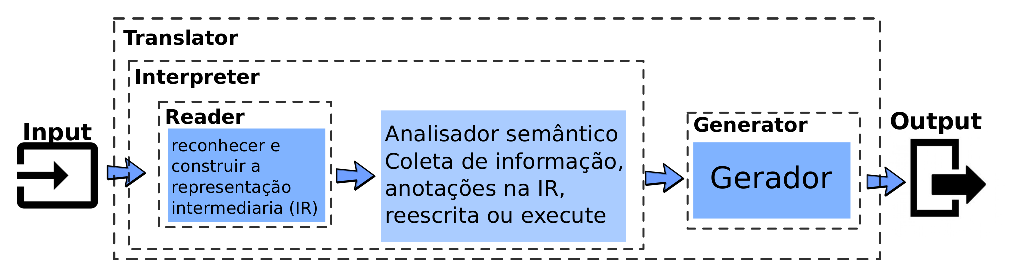
\includegraphics[scale=0.9]{Imagens/stagesLanguageApp}
  \label{fig:stagesLanguageApp}
  \caption{Fases de aplicaç\~{o}es com linguagens.}
\end{figure}

Existe um esforço consider\'{a}vel para tratar a engenharia de linguagens de programaç\~{a}o como sendo o desenvolvimento de um software comum. 
Algumas aplicaç\~{o}es t\'{i}picas deste dom\'{i}nio s\~{a}o \texttt{reconhecedores, interpretadores, tradutores e geradores}, 
conforme menciona Terrance Parr~\cite{Parr:2009:LIP:1823613}. 

%% Um \emph{Reconhecedor} \'{e} uma construç\~{a}o capaz de receber uma estrutura de dado como um input ou um fluxo de inputs. O fluxo de input pode geralmente \'{e} texto puro mas pode ser utilizado dado bin\'{a}rio. Como exemplo de aplicaç\~{a}o tem-se ferramentas analisadoras de referências cruzadas, e ferramentas para carregar classes.

%% \texttt{Interpretador:} Um interpretador, lê uma entrada, decodifica e executa as instruç\~{o}es, interpretadores variam de simples calculadoras at\'{e} a implementaç\~{a}o de linguagens de programaç\~{a}o como Java, Python e PHP.

%% \texttt{Tradutor:}A partir um input de texto ou bin\'{a}rio \'{e} emitido uma sa\'{i}da para uma linguagem que pode ser a mesma ou n\~{a}o. É a combinaç\~{a}o do \textit{reader} e \textit{generator}. Como exemplo tem-se tradutores de linguagens extintas para linguagens atuais, \texttt{refactorers},  gerador de logs e macro pre-processadores.
	
%% \texttt{Gerador:} Percorre uma estrutura de dado e emite uma sa\'{i}da. Como exemplo tem-se ferramentas de mapeamento de objetos relacionais em banco de dados, serializador de objetos, gerador de c\'{o}digo fonte e geradores de p\'{a}gina web.



Al\'{e}m dessas aplica\c c\~{o}es t\'{i}picas, 
ferramentas para a identifica\c c\~{a}o est\'{a}tica de \emph{bugs}, por exemplo, tamb\'{e}m s\~{a}o comumente 
implementadas usando uma organiza\c c\~{a}o como a representada na Figura~\ref{fig:stagesLanguageApp}. 
A ferramenta \textit{FindBugs}~\cite{FindBugs} serve como um exemplo de solu\c c\~{a}o para identifica\c c\~{a}o 
de poss\'{i}veis erros em programas escritos na linguagem Java, a partir do \emph{bytecode} resultante do 
processo de compila\c c\~{a}o. Note na Figura:~\ref{fig:findBugs} a semelhan\c ca arquitetural com as 
abordagens t\'{i}picas para o processamento de artefatos de linguagens de programa\c c\~{a}o. 

\begin{figure}[h]
	\center
	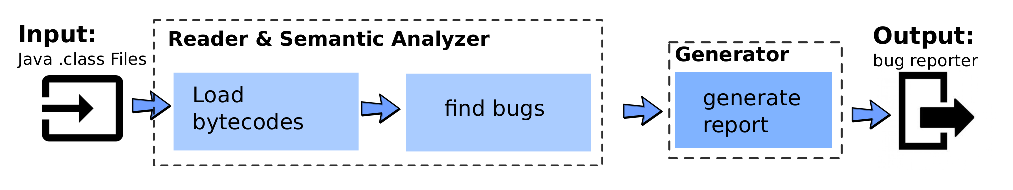
\includegraphics[scale=0.9]{Imagens/pipelineFindbugs}
	\label{fig:findBugs}
	\caption{Fase do pipiline do FindBugs.}
\end{figure}


Especificamente no caso deste trabalho, percebeu-se a necessidade de construç\~{a}o de um software que 
realiza a an\'{a}lise est\'{a}tica de c\'{o}digo para identificar tanto o uso quanto as oportunidades do uso de construç\~{o}es 
sint\'{a}ticas / sem\^{a}nticas da linguagem Java. Em termos arquiteturais, a Figura:~\ref{fig:stagesAnalyzer} ilustra, 
em um alto n\'{i}vel de abstra\c c\~{a}o, os principais componentes que formam o \emph{pipeline} do analisador est\'{a}tico 
implementado nesse trabalho e cujos detalhes de implementa\c c\~{a}o s\~{a}o apresentados no pr\'{o}ximo cap\'{i}tulo.

\begin{figure}[h]
	\center
	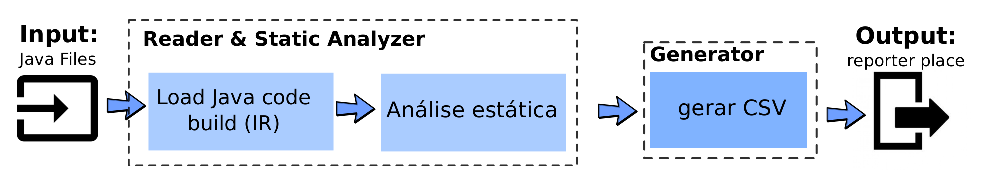
\includegraphics[scale=0.9]{Imagens/stagesAnalizer}
	\label{fig:stagesAnalyzer}
	\caption{Ferramentas necess\'{a}rias para construç\~{a}o do analisador est\'{a}tico.}
\end{figure}


Pode-se compreender este analisador como um \emph{grammarware} pois \'{e} um software 
que depende fortemente de uma gram\'{a}tica para seu funcionamento neste caso a gram\'{a}tica da linguagem Java. 
%\emph{Grammawares} demandam um conhecimento essencial das  gram\'{a}ticas que manipulam. 
%Como exemplos de arquiteturas que possuem tal conhecimento tem-se os programas de convers\~{a}o de dados, processadores de \texttt{XML} e os que efetuam \textit{parses}.
De acordo com Paul Klint et al~\cite{klint2005toward}, alguns cen\'{a}rios favorecem o desenvolvimento de softwares alinhados com a abordagem 
\emph{grammarware}, com destaque \`{a}s aplicaç\~{o}es que necessitam importar perfis de usu\'{a}rios para promover a transiç\~{a}o da vers\~{a}o 
antiga para uma vers\~{a}o nova. 
Esta transiç\~{a}o deve ser robusta e provavelmente necessitar\'{a} de adptaç\~{a}o dever\'{a} passar 
por um parser para que as partes que necessitem de adaptaç\~{a}o possam ser identificadas.

Um outro cen\'{a}rio real \'{e} o desenvolvimento de aplicaç\~{o}es de banco de dados onde se faz necess\'{a}rio adotar 
uma nova linguagem de definiç\~{a}o para um ambiente espec\'{i}fico. De forma que automatizar esta soluç\~{a}o requer o uso de um 
parser que ser\'{a} respons\'{a}vel por reconhecer as entradas necess\'{a}rias para efetuar o mapeamento 
para a \emph{linguagem} destino.


%% Um \textit{software} que efeta manipula\c{c}\~{a}o da gram\'{a}tica de uma linguagem, como no caso deste trabalho de conclus\~{a}o fica evidente o aparecimento da quest\~{a}o sobre \textit{refactoring} e dentre diversas caracter\'{i}sitas explicadas por Martin Fowler~\cite{martinFowlerRafactoring}, fica claro que este trabalho contribui com o intu\'{\i}to de identificar constru\c{c}\~{o}es obsoletas n\~{a}o efetuando \textit{refactoring} autom\'{a}tico mas fazendo  com que o desenvolvedor opte pela evolu\c{c}\~{a}o ou n\~{a}o. Pois a evolu\c{c}\~{a}o do c\'{o}digo por um mais atual \'{e} uma das oportunidades de melhorar o desgin do \textit{software} conforme aborda por Martin Fowler~\cite{martinFowlerRafactoring} em seu livro.

%% Mesmo sem a implementa\c{c}\~{a}o de \textit{refactoring} uma contribui\c{c}\~{a}o que este trabalho faz \'{e} a identifi\c{c}\~{a}o a capacidade de encontrar c\'{o}digo duplicado como por exemplo ao identificar \texttt{catch} repetidos, ou at\'{e} mesmo melhorar o desempenho com no caso da da utilizaç\~{a}o do \texttt{switch-string} ao inv\'{e}s do \texttt{if-string} pois oracle afirma que o desempenho \'{e} melhor de a implementa\c{c}\~{a}o otimizada do \texttt{switch-string} na documenta\c{c}\~{a}o~\cite{docSwitch}.




%Atualmente a evoluç\~{a}o de uma linguagem de programaç\~{a}o ocorre predominantemente de forma {\it ad-hoc} e em muitos casos manualmente, para a traduç\~{a}o de aplicativos legados, conforme a demanda. A ferramentas de an\'{a}lise para gerar a evoluç\~{a}o necess\'{a}ria, {\it grammarware}, tende a condizir este processo abordando a classe gramatical que deve ser evolu\'{i}da. Neste caso analisador que muitas vezes realizaria o trabalho por tentativa e erro, tem como base a gram\'{a}tica do c\'{o}digo a ser analisado. Especificaç\~{o}es do analisador s\~{a}o derivados automaticamente da semi gram\'{a}tica. Diferentes tecnologias de an\'{a}lise que podem ser orientadas em oposiç\~{a}o a uma tecnologia espec\'{i}fica. Assim o processo de personalizaç\~{a}o/evoluç\~{a}o \'{e} suscept\'{i}vel de exigir a entrada de um engenheiro de {\it grammarware} o qual tem conhecimento pr\'{e}vio da gram\'{a}tica a ser analisada.

%Um ponto cr\'{i}tico quanto a an\'{a}lise de c\'{o}digo fonte \'{e} o \textit{parser} da linguagem, onde \'{e} necess\'{a}rio reconhecer uma frase para efetuar a interpretaç\~{a}o ou fazer a traduç\~{a}o para que a criaç\~{a}o da representaç\~{a}o intermedi\'{a}ria aconteça. Inicialmente \'{e} necess\'{a}rio identificar se a frase que ser\'{a} tratada \'{e} um \textit{assignment} ou uma chamada de funç\~{a}o.
 
%Reconhecer uma frase acarreta em duas coisas, distingui-la de outras construç\~{o}es e identificar os elementos e as subestruturas que comp\~{o}em esta frase. Por exemplo se uma frase for reconhecida como um \textit{assignment}, pode-se identificar as vari\'{a}veis a esquerda do operador \texttt{=} e uma express\~{a}o que \'{e} a subestrutura a direita. Este ato de reconhecer uma frase \'{e} denominado \textit{Parse}.


\section{Parse}

Confome discutido anteriormente, o parser de programas escritos em uma linguagem de program\c c\~{a}o 
\'{e} um dos componentes necess\'{a}rios para a constru\c c\~{a}o de ferramentas de an\'{a}lise 
est\'{a}tica. Vale ressaltar que o analisador est\'{a}tico constru\'{i}do neste trabalho reusou uma infraestrutura 
da plataforma Eclipse que oferece um parser atualizado da linguagem Java. Por outro lado, como 
se trata de um tipo de componente central para solu\c c\~{o}es baseadas em gram\'{a}tica, esta se\c c\~{a}o 
revisa brevemente quatro padr\~{o}es adotados para a implementa\c c\~{a}o de parsers segundo Terence Parr~\cite{Parr:2009:LIP:1823613}. S\~{a}o eles: 

\begin{itemize}
	\item \textbf{Mapping Grammars to Recursive-Descent Recognizers}\\

	Sua proposta \'{e} traduzir uma gram\'{a}tica para uma implementa\c c\~{a}o que usa recurs\~{a}o descendente 
para reconhecer frases e sentenças em uma linguagem especifica. Este padr\~{a}o identifica o n\'{u}cleo do fluxo de controle 
para qualquer recurs\~{a}o descendente e \'{e} utilizado nos 3 padr\~{o}es seguintes. Para construir um reconhecedor l\'{e}xico ou \textit{parsers} 
manualmente o melhor ponto de in\'{i}cio \'{e} a gram\'{a}tica, com isso este padr\~{a}o fornece uma maneira simples de construir reconhecedores diretamente de sua gram\'{a}tica.
	
	\item \textbf{LL(1) Recursive-Descent Lexer}\\

	O objetivo deste padr\~{a}o \'{e} emitir uma sequência de s\'{i}mbolos. Cada s\'{i}mbolo tem dois atributos prim\'{a}rios: 
um tipo de \textit{token} (s\'{i}mbolo da categoria) e o texto associado por exemplo 
	no português, temos categorias como verbos e substantivos, bem como s\'{i}mbolos de pontuaç\~{a}o, como v\'{i}rgulas e pontos. Todas as palavras dentro de uma determinada categoria s\~{a}o do mesmo tipo de \textit{token}, embora o texto associado seja diferente. O tipo de nome do \textit{token} representa o categoria identificador. Ent\~{a}o precisamos tipos de \textit{token} para o vocabul\'{a}rio \textit{string} fixa s\'{i}mbolos como tamb\'{e}m lidar com espaços em branco e coment\'{a}rios.
	\item \textbf{LL(1) Recursive-Descent Parser}\\
	Esse \'{e} o mais conhecido padr\~{a}o de an\'{a}lise descendente recursiva. Ele s\'{o} precisa	a olhar para o s\'{i}mbolo de entrada atual para tomar decis\~{o}es de an\'{a}lise. Para cada regra de gram\'{a}tica, existe um m\'{e}todo de an\'{a}lise no analisador. Este padr\~{a}o analisa a estrutura sint\'{a}tica da sequência sinal de uma frase usando um \'{u}nico \textit{token} \textit{lookahead}. Este analisador pertence à LL(1) classe do analisador de cima para baixo, em especial, porque usa um \'{u}nico sinal de verificaç\~{a}o à frente (da\'{i} o "1" no nome). É o principal mecanismo de todos os padr\~{o}es de an\'{a}lise subsequentes. Este padr\~{a}o mostra como implementar as decis\~{o}es de an\'{a}lise que utilizam um s\'{i}mbolo \'{u}nico da vis\~{a}o antecipada. É a forma mais fraca de descendente recursivo parser, mas o mais f\'{a}cil de compreender e aplicar.
	\item \textbf{LL(k) Recursive-Descent Parser}\\
	Este padr\~{a}o utiliza a o modo \textit{top-down} para percorrer um \'{a}rvore sem\^{a}ntica com o aux\'{i}lio de express\~{o}es booleanas que ajudam na tomada de decis\~{a}o e estas express\~{o}es s\~{a}o conhecidas como predicados sem\^{a}nticos.
	
\end{itemize}



\section{Refactoring}\label{sec:refactoring}

Por defini\c{c}\~{a}o o \textit{refactoring} \'{e} mudan\c{c}a interna do software sem alterar seu comportamento tornando assim seu entendimento mais claro. Visando evitar que sejam perdidas diversa horas para identificar poss\'{\i}veis oportunidades de classes onde possam ser evolu\'{\i}das, este trabalho de conclus\~{a}o identifica trechos de c\'{o}digo dentro das classes que podem ser evolu\'{i}dos.

Muitas modifica\c{c}\~{o}es podem ser feitas em um software mas segundo M.Fowler et al~\cite{martinFowlerRafactoring} somente \'{e} considerado \textit{refactoring} mudan\c{c}as que facilitam o entendimento do software. Contrastando esta vis\~{a}o existem mudan\c{c}as com objetivo de melhorar o desempenho do software onde somente s\~{a}o alterada as estruturas internas permanecendo inalterado o comportamento do software. Entretanto a melhoria na performance do software geralmente eleva o grau de dificuldade para sua compreens\~{a}o, o que faz com que algumas dessas evolu\c{c}\~{o}es visando desempenho n\~{a}o sejam caracterizadas como \textit{refactoring} dado a defini\c{c}\~{a}o.

Dentre refatorar para facilitar o entendimento, para tornar o programa mais r\'{a}pido, para encontrar bugs e para melhorar/atualizar o design, motivos apresentados por M.Fowler et al~\cite{martinFowlerRafactoring}, este trabalho concentrou-se no \'{u}ltimo motivo para identificar poss\'{\i}veis casos onde o design do software pode ser evolu\'{\i}do por substituir funcionalidades de vers\~{o}es anteriores da linguagem Java.

Um software que n\~{a}o \'{e} refatorado tem o seu desgin deteriorado, o que leva a dificultar o entendimento do c\'{o}digo. Um design ultrapassado tem mais c\'{o}digo que o necess\'{a}rio para realizar a mesma tarefa. O que leva a um aspecto crucial para a melhoria, que \'{e} código duplicado. Vale ressaltar que reduzir a quantidade de c\'{o}digo n\~{a}o impl\'{i}ca necessariamente na melhora do desempenho do software mas sim em ter um design mais atual.

O Listing:~\ref{lst:fp}, exemplifica de forma emp\'{i}rica um {\it filter} em um {\it collection} onde ocorre uma redu\c{c}\~{a}o significativa de c\'{o}digo al\'{e}m de um design mais atual por utilizar express\~{o}es lambda que foram adicionadas em Java 8. Vale destacar que o Listing:~\ref{lst:fp} continua com mesmo comportamento ap\'{o}s o \textit{refactoring}, desta forma nenhum usu\'{a}rio ou desenvolvedor pode alegar que o software foi modificado.


\begin{lstlisting}[caption={The \textsc{Exmplo de Filter Pattern}}\label{lst:fp},language=Java] 
//...
for(T e: collection) {
   if(e.pred(args)) {
      otherCollection.add(e);
   }
}

//might be replaced by:
collection.stream().
	filter(e->pred(args).
		forEach(e -> otherCollection.add(e));
\end{lstlisting}


Conforme explica M.Fowler et al~\cite{martinFowlerRafactoring} algumas vezes n\~{a}o se deve ser refatorar o c\'{o}digo. Um desses casos \'{e} quando existir a necessidade de reescrever todo o c\'{o}digo, um outro caso \'{e} a necessidade de manter um  c\'{o}digo de f\'{a}cil entendimento para os programadores iniciantes. O que \'{e} uma decis\~{a}o dif\'{i}cil, no caso do Listing:~\ref{lst:fp} \'{e} poss\'{\i}vel fazer uma evolu\c{c}\~{a}o com caracter\'{i}sticas funcionais introduzidas em Java 8 entretanto alguns desenvolvedores podem n\~{a}o possuir  conhecimento adequado de tal funcionalidade e com isso \'{e} recomendado que n\~{a}o seja evolu\'{\i}do o c\'{o}digo.


Tendo em vista que aplicar um \textit{refactoring} demanda tempo isto torna uma tarefa custosa para empresas, este fator \'{e} determinante para que programadores n\~{a}o refatorem seu c\'{o}digos em muitos casos. Com esse cen\'{a}rio \'{e} imprecind\'{i}vel o uso de ferramentas que refatorem ou auxiliem nesta tarefa. Auxiliando nesta tarefa este trabalho identifica possibilidades de refatora\c{c}\~{a}o, ao utilizarem estas ferramentas torna mais acessível ao programador e a emrpesa refatorar pois o trabalho é direcionado fazendo com que tempo seja poupado.



\section{Análise estática}\label{sec:as}

Em computa\c{c}\~{a}o an\'{a}lise est\'{a}tica \'{e} a refer\^{e}ncia a qualquer processamento realizado em c\'{o}digo fonte sem a necessidade de execut\'{a}-lo, com isto a an\'{a}lise est\'{a}tica torna-se uma poderosa t\'{e}cnica por permitir r\'{a}pidas considera\c{c}\~{o}es por possibilitar uma larga explora\c{c}\~{a}o em um projeto podendo evitar erros triviais e simular alguns cen\'{a}rios para tal an\'{a}lise sem a necessidade do projeto ser executado.

Ferramentas que auxiliem a an\'{a}lise est\'{a}tica tem grande chance de ser um poderoso aux\'{i}lio no desenvolvimento do software tendo em vista que pode reduzir a quantidade de erros e diminuir a quantidade de \textit{refactoring} o qual tem um custo elevado para os projetos de software.

\'{E} nesse contexto que este trabalho faz sua contribui\c{c}\~{a}o por utilizar a an\'{a}lise est\'{a}tica para verificar n\~{a}o a possibilidade de falhas ou \textit{bad smell}, mas sim de identificar chances reais de evoluir para \'{u}ltimas \textit{features} da linguagem Java sem interferir no comportamento interno do programa conforme preconiza M.Fowler et al~\cite{martinFowlerRafactoring}.

A linguagem Java proporciana duas maneiras de realizar an\'{a}lise est\'{a}tica, a primeira \'{e} através c\'{o}digo fonte, \textit{.java} e a segunda atrav\'{e}s do \textit{bytecode}, \textit{.class}. Este trabalho foca em realizar an\'{a}lise no c\'{o}digo fonte, entre tanto nada impede que o trabalho seja realizado da segunda maneira. Existem programas renomados que realizam tal an\'{a}lise utilizando os \textit{bytecodes} e um destes programas \'{e} o FindBugs~\cite{FindBugs}.

%Análise estática é uma técnica automática no processo de verifica\c{c}ão de software realizado por algumas ferramentas sem a necessidade de que o software tenha sido executado. Para Java exitem duas possibilidades de realizar tal análise na qual uma das técnicas realiza a primeira \'{e} aanálise no código fonte e a outra a realiza no {\it bytecode} do programa segundo N. Ayewah et al ~\cite{Ayewah:2008:USA:1439186.1439221}. Neste trabalho ser utilizada a pesquisa baseada no código fonte sem que tenha sido executado devido a flexibilidade e infraestrutura consolidada encontrada no Eclipse AST.

Para obter sucesso atrav\'{e}s das an\'{a}lises realizadas, \'{e} necess\'{a}rio determinar padr\~{o}es para encontrar caracter\'{i}sticas que dejesam ser evolu\'{i}das para a \'{u}ltima vers\~{a}o da linguagem Java. Estes padr\~{o}es s\~{a}o estabelecidos em uma estrutura que seja capaz de pesquisar nos n\'{o}s da \'{a}rvore da representa\c{c}\~{a}o intermedi\'{a}ria para extrair as informa\c{c}\~{o}es pertinentes.

%Um fato importante é que tal análise somente obt\'{e}m sucesso se forem determinados padr\~{o}es ou comportamento para que sejam pesquisados no software. Neste projeto o tais comportamentos são determinados por {\it visitors} conforme explica Gamma et al ~\cite{Gamma:1995} devido a toda infraestrutura a qual as ferramentas do eclipse fornecem facilidade para que seja realizada uma análise baseada em padrões.

A t\'{e}cnica utilizada para pesquisar nos n\'{o}s das \'{a}rvores foi utilizar o padr\~{a}o de projeto \textit{Visitor} proposto por  Gamma et al~\cite{Gamma:1995}, pois este possibilitar que seja realizada uma opera\c{c}\~{a}o sobre todos os elementos de uma estrutura,  neste caso a opera\c{c}\~{a}o  \'{e} a pesquisa e a estrutura a representa\c{c}\~{a}o intermedi\'{a}ria.


A verifica\c{c}\~{a}o de software possibilita a detec\c{c}\~{a}o de falhas de maneira precoce durante as fases de desenvolvimento entretanto este n\~{a}o \'{e} o objetivo deste trabalho pois existem ferramentas consolidadas que realizam tal an\'{a}lise de maneira excepcional. Aqui o objetivo principal \'{e} alertar ao desenvolvedor a possibilidade de usar o que h\'{a} de mais recente na linguagem Java.

%Devido a este trabalho de verifica\c{c}ão de software é possível detectar falhas de forma precoce nas fases de  desenvolvimento evitando que bugs e falhas sejam introduzidas e até mesmo postergados e isso é uma vantagem existe a economia de tempo com falhas simples, {\it  feedback} rápido para alertar a equipe devido as falhas ocorridas e pode-se ir além de simples casos de testes podendo aprimorar estes para que  fiquem mais rigorosos pois a partir do momento que o analisador encontrar uma falha é possível criar um teste de caso para que esta seja testada aumentando a confiabilidade do software.

%Existe limita\c{c}\~{a}o quanto a capacidade dos analisadores est\'{a}ticos como em \textit{software} desenvolvidos sem qualquer uso de padrões ou sem arquiteturas consolidadas, criado por equipes composta de desenvolvedores inexperientes o qual a ferramente poderá apontar erros que são falsos positivos que são erros detectados que não existem pois o analisador pesquisa por padrões e estruturas consolidadas. Tais problemas são desagradáveis porém não oferecem riscos ao desenvolvimento, podem afetar outras áreas como a de {\it refactoring} a qual poderá encontrar dificuldade em melhorar um código que não segue padrão. Vale ainda ressaltar que a penalidade de encontrar um falso positivo é a perda de tempo em fazer uma inspe\c{c}ão no código para comprovar se é ou não uma falha. Também há a possibilidade de falsos negativos o que cabe ao programador verificar para evitar que tais limitação do analisador não se propague durante o ciclo de desenvolvimento.


%A capacidade dos analisadores est\'{a}ticos 


%	\section {Análise léxica}
	Ferramentas que operam em código-fonte conforme \cite{Wichmann95industrialperspective} começam por transformar o código em um série de {\it tokens}, descartando recursos sem importância de o texto do programa, tais como espaços em branco ou comentários ao longo do caminho. A criação do fluxo de sinal é chamado de análise lexical. Regras léxicas muitas vezes usam expressões regulares para identificar fichas.
	Observa-se que a maioria dos {\it tokens} são representados inteiramente por seu tipo, mas para ser útil, o {\it tokens} de identificação requer uma peça adicional de informação: o nome do identificador. Para habilitar o relatório de erro útil mais tarde, os {\it tokens} devem transportar pelo menos um outro tipo de informação com eles: a sua posição no texto-fonte (geralmente um número de linha e um número de coluna). Para as mais simples ferramentas de análise estática, o trabalho está quase concluído neste ponto. Se toda a ferramenta tem que fazer é combinar os nomes de funções, o analisador pode ir através do fluxo de {\it tokens} procurando identificadores, combiná-los com uma lista de nomes de funções, e relatar o resultados.
	
	\section{Parser}
	Um analisador de linguagem usa uma gramática livre de contexto (CFG) indicado por \cite{Chess:2007:SPS:1406221} para coincidir com os {\it tokens} correntes. A gramática é composta por um conjunto de produções que descrevem os símbolos (elementos) na língua. No Exemplo é enumerado um conjunto de produções que são capazes de analisar o fluxo de {\it tokens} de amostra.
	
	\begin{lstlisting}
	stmt := if_stmt | assign_stmt
	if_stmt := IF LPAREN expr RPAREN stmt
	expr := lval
	assign_stmt := lval EQUAL expr SEMI
	lval = ID | arr_access
	arr_access := ID arr_index+
	arr_idx := LBRACKET expr RBRACKET
	\end{lstlisting}
	
	O analisador executa uma derivação, combinando o fluxo de sinal contra as regras de produção. Se cada símbolo é ligado a partir da qual o símbolo foi derivado, uma árvore de análise é formada. Na Figura: \ref{fig:TreeParser} mostra uma árvore de análise criada, usando as regras de produção do exemplo anterior. Omiti-se terminais de símbolos que não carregam nomes \textit{(IF, LPAREN, RPAREN, etc.}), para fazer o principais características da árvore de análise mais óbvia.
	
	\begin{figure}[h]
		\center
		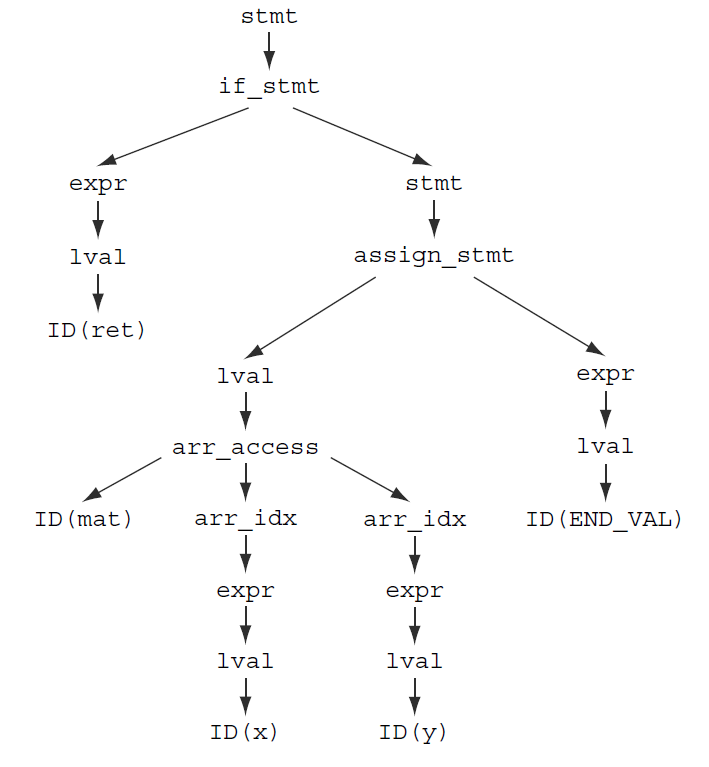
\includegraphics[width=0.8\textwidth]{Imagens/Arvore}
		\label{fig:TreeParser}
		\caption{Árvore de parser.}
	\end{figure}
	
	
	\subsection{Paser JDT Eclipse}
	No caso do \textit{parser} provido pela infraestrutura \textit{JDT} do eclipse,  a classe \textit{ASTParser} contida na biblioteca \textit{org.eclipse.jdt.core.dom} permite a criação de uma árvore de sintaxe abstrata.\\
	Este procedimento é realizado em todos os aquivos \textit{.java} contido em um projeto e com isso cada um possui uma referência de \textit{CompilationUnit} o qual permite acesso ao nó raiz árvore sintática de cada arquivo. O parse é gerado conforme as últimas definições da linguagem utilizando \textit{AST.JLS8}.\

	\begin{lstlisting}
		ASTParser parser = ASTParser.newParser(AST.JLS8);
		
		Map<String, String> options = JavaCore.getOptions();
		options.put(JavaCore.COMPILER_COMPLIANCE, JavaCore.VERSION_1_8);
		options.put(JavaCore.COMPILER_CODEGEN_TARGET_PLATFORM, JavaCore.VERSION_1_8);
		options.put(JavaCore.COMPILER_SOURCE, JavaCore.VERSION_1_8);
		
		parser.setKind(ASTParser.K_COMPILATION_UNIT);
		parser.setCompilerOptions(options);
		parser.setSource(contents);
		
		final CompilationUnit cu = (CompilationUnit) parser.createAST(null);
		return cu;
	\end{lstlisting}
	
	Neste, o \textit{parser} é realizado através de uma classe denominada de mesmo nome, a qual é instanciada um única vez no projeto através do padrão \textit{singleton} \cite{Gamma:1995}.
	

	\section{Sintaxe abstrata}
	É possível fazer uma análise significativa em uma árvore de parser, e certos tipos de checagem estilísticas são mais bem executadas em uma árvore de análise, pois contém mais representações diretas do código assim como o programador escreve. No entanto, executar análise complexa em uma árvore de análise pode ser inconveniente. Os nós da árvore são derivados diretamente das regras de produção da gramática, e essas regras podem-se introduzir símbolos não terminais que existem apenas para fins de fazer a análise mais fácil e menos ambígua, ao invés de para o objetivo de produzir uma facilmente compreendido a árvore. É geralmente melhor para abstrair ambos os detalhes da gramática e as estruturas sintáticas presente no código fonte do programa. Uma estrutura de dados que faz estas coisas é chamado de uma árvore de sintaxe abstrata (AST). O objectivo da AST é fornecer uma versão padronizada do programa adequado para posteriores análises. A AST é normalmente construída associando código construção árvore com regras de produção da gramática. A Figura: \ref{fig:ArvoreAST} mostra uma AST. Observa-se que a instrução {\it if} agora tem uma outra ramificação vazia, o predicado testado pelo caso é agora uma comparação explícita para zero (o comportamento exigido pelo C), e acesso à matriz é uniformemente representada como uma operação de binário.
	
	\begin{figure}[h]
		\center
		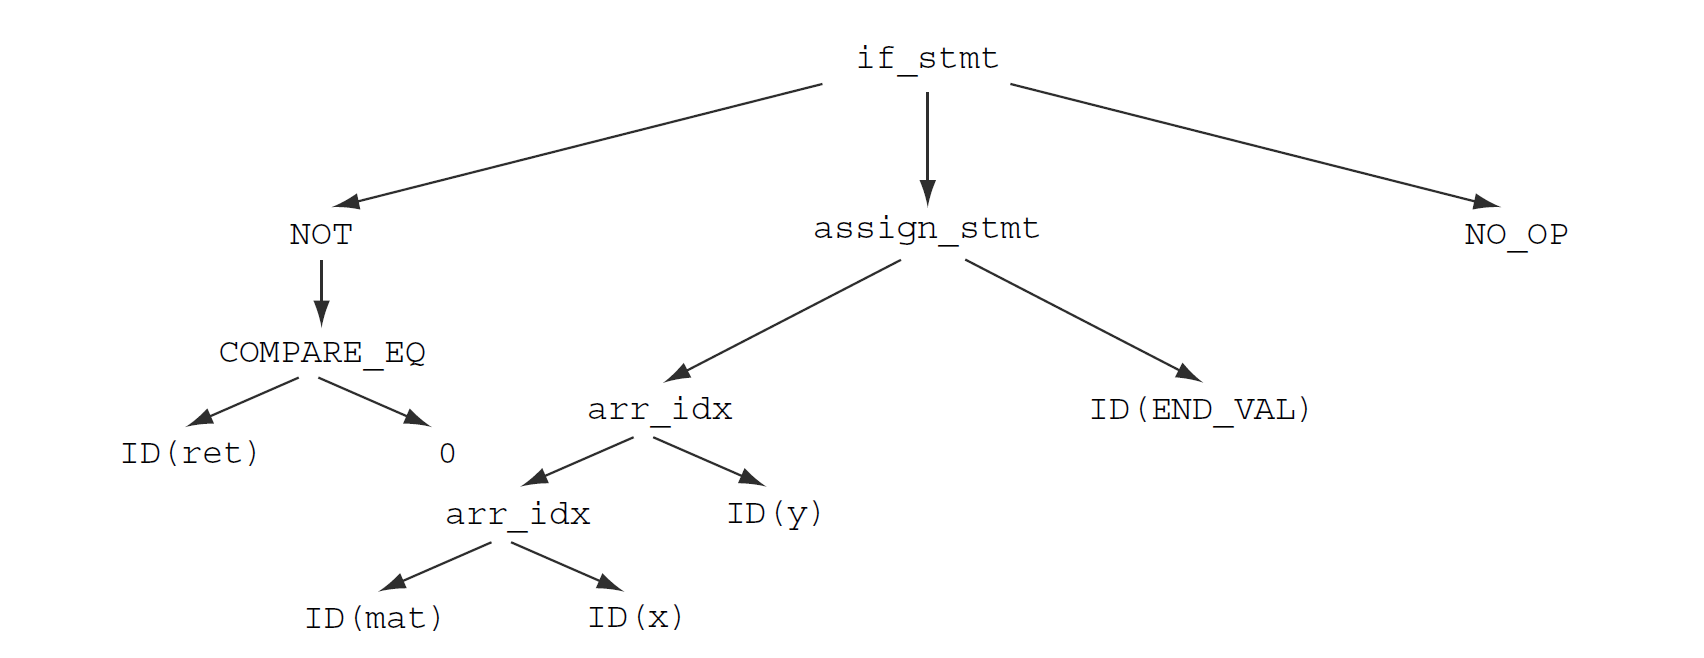
\includegraphics[width=1\textwidth]{Imagens/ArvoreAST}
		\label{fig:ArvoreAST}
		\caption{Árvore AST.}
	\end{figure}

	\section{Análise semântica}
	Como a AST está sendo construída, a ferramenta cria uma tabela de símbolos ao lado dela. Para cada identificador no programa, a tabela de símbolos associa o identificador com seu devido tipo e um ponteiro para a sua declaração ou definição. Com a AST e a tabela de símbolo, a ferramenta está agora equipado-se para realizar a verificação de tipo. A ferramenta de análise estática não pode ser obrigados a comunicar erros de checagem de tipo da maneira um compilador faz, mas informações de tipo é criticamente importante para a análise de uma linguagem orientada a objetos, porque o tipo de um objeto determina o conjunto de métodos que o objeto pode invocar. Além disso, é normalmente desejável para converter, pelo menos, as conversões do tipo implícito no código fonte para conversões de tipo explícitas no AST. Por estas razões, uma ferramenta de análise estática avançado tem a ver apenas como muito trabalho relacionado com a verificação de tipo como um compilador faz. No mundo do compilador, resolução de símbolo e verificação de tipo são referidos como análise semântica porque o compilador está atribuindo significado aos símbolos encontrada no programa. As ferramentas de análise estática que usam essas estruturas de dados têm uma vantagem distinta sobre ferramentas que não o fazem. Por exemplo, eles podem interpretar corretamente o significado dos operadores sobrecarregados em C++ ou determinar que um método em Java chamado doPost () é, na verdade, uma parte de uma implementação de HttpServlet.Estas capacidades permitem uma ferramenta para executar verificações úteis na estrutura deo programa. Após análise semântica, compiladores e a análise estática mais avançada ferramentas de formas de peça. Um compilador moderno usa a AST e o símbolo e o tipo informações para gerar uma representação intermediaria, uma versão genérico do código de máquina que é adequado para otimização e, em seguida, a conversão em específico da plataforma de código-objeto. O caminho para ferramentas de análise estática é menos clara. Dependendo do tipo de análise a ser realizada, uma ferramenta de análise estática pode executar transformações adicionais sobre a AST ou pode gerar a sua própria variedade de representação intermediária adequada às suas necessidades. Se uma ferramenta de análise estática usa sua própria representação intermediária, que, geralmente, permite a atribuição, pelo menos, ramificando, {\it looping}, e chamadas de função. A representação intermediária que uma ferramenta de análise estática usa é geralmente umvista de nível superior do programa do que a representação intermediária que um compilador usa. Por exemplo, um compilador de linguagem C, provavelmente, converter todas as referências a campos para estruturar deslocamentos em {\it byte} na estrutura pela sua representação intermediaria, enquanto uma ferramenta de análise estática mais provavelmente continuará para se referir a estrutura de campos, pelos seus nomes.%	\section {Análise léxica}
	Ferramentas que operam em código-fonte conforme \cite{Wichmann95industrialperspective} começam por transformar o código em um série de {\it tokens}, descartando recursos sem importância de o texto do programa, tais como espaços em branco ou comentários ao longo do caminho. A criação do fluxo de sinal é chamado de análise lexical. Regras léxicas muitas vezes usam expressões regulares para identificar fichas.
	Observa-se que a maioria dos {\it tokens} são representados inteiramente por seu tipo, mas para ser útil, o {\it tokens} de identificação requer uma peça adicional de informação: o nome do identificador. Para habilitar o relatório de erro útil mais tarde, os {\it tokens} devem transportar pelo menos um outro tipo de informação com eles: a sua posição no texto-fonte (geralmente um número de linha e um número de coluna). Para as mais simples ferramentas de análise estática, o trabalho está quase concluído neste ponto. Se toda a ferramenta tem que fazer é combinar os nomes de funções, o analisador pode ir através do fluxo de {\it tokens} procurando identificadores, combiná-los com uma lista de nomes de funções, e relatar o resultados.
	
	\section{Parser}
	Um analisador de linguagem usa uma gramática livre de contexto (CFG) indicado por \cite{Chess:2007:SPS:1406221} para coincidir com os {\it tokens} correntes. A gramática é composta por um conjunto de produções que descrevem os símbolos (elementos) na língua. No Exemplo é enumerado um conjunto de produções que são capazes de analisar o fluxo de {\it tokens} de amostra.
	
	\begin{lstlisting}
	stmt := if_stmt | assign_stmt
	if_stmt := IF LPAREN expr RPAREN stmt
	expr := lval
	assign_stmt := lval EQUAL expr SEMI
	lval = ID | arr_access
	arr_access := ID arr_index+
	arr_idx := LBRACKET expr RBRACKET
	\end{lstlisting}
	
	O analisador executa uma derivação, combinando o fluxo de sinal contra as regras de produção. Se cada símbolo é ligado a partir da qual o símbolo foi derivado, uma árvore de análise é formada. Na Figura: \ref{fig:TreeParser} mostra uma árvore de análise criada, usando as regras de produção do exemplo anterior. Omiti-se terminais de símbolos que não carregam nomes \textit{(IF, LPAREN, RPAREN, etc.}), para fazer o principais características da árvore de análise mais óbvia.
	
	\begin{figure}[h]
		\center
		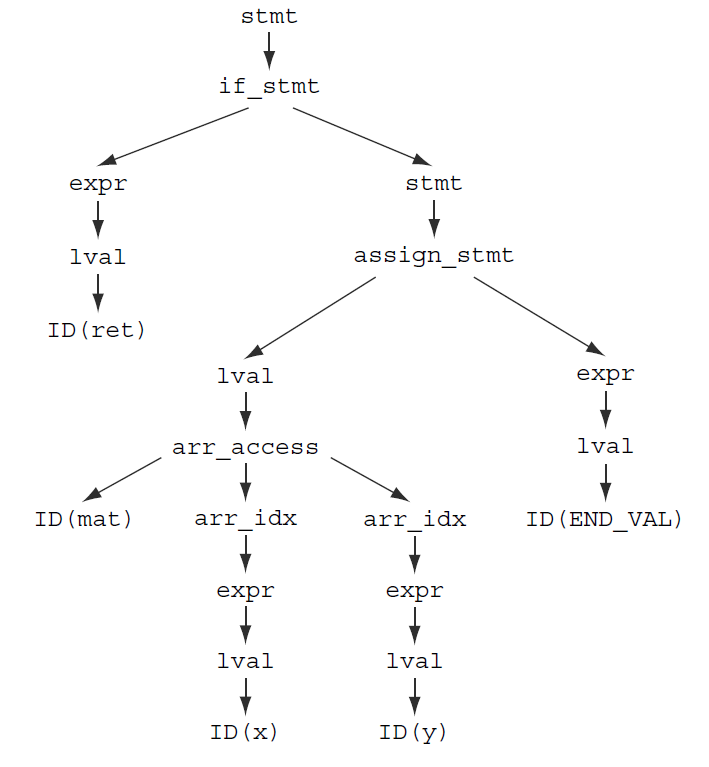
\includegraphics[width=0.8\textwidth]{Imagens/Arvore}
		\label{fig:TreeParser}
		\caption{Árvore de parser.}
	\end{figure}
	
	
	\subsection{Paser JDT Eclipse}
	No caso do \textit{parser} provido pela infraestrutura \textit{JDT} do eclipse,  a classe \textit{ASTParser} contida na biblioteca \textit{org.eclipse.jdt.core.dom} permite a criação de uma árvore de sintaxe abstrata.\\
	Este procedimento é realizado em todos os aquivos \textit{.java} contido em um projeto e com isso cada um possui uma referência de \textit{CompilationUnit} o qual permite acesso ao nó raiz árvore sintática de cada arquivo. O parse é gerado conforme as últimas definições da linguagem utilizando \textit{AST.JLS8}.\

	\begin{lstlisting}
		ASTParser parser = ASTParser.newParser(AST.JLS8);
		
		Map<String, String> options = JavaCore.getOptions();
		options.put(JavaCore.COMPILER_COMPLIANCE, JavaCore.VERSION_1_8);
		options.put(JavaCore.COMPILER_CODEGEN_TARGET_PLATFORM, JavaCore.VERSION_1_8);
		options.put(JavaCore.COMPILER_SOURCE, JavaCore.VERSION_1_8);
		
		parser.setKind(ASTParser.K_COMPILATION_UNIT);
		parser.setCompilerOptions(options);
		parser.setSource(contents);
		
		final CompilationUnit cu = (CompilationUnit) parser.createAST(null);
		return cu;
	\end{lstlisting}
	
	Neste, o \textit{parser} é realizado através de uma classe denominada de mesmo nome, a qual é instanciada um única vez no projeto através do padrão \textit{singleton} \cite{Gamma:1995}.
	

	\section{Sintaxe abstrata}
	É possível fazer uma análise significativa em uma árvore de parser, e certos tipos de checagem estilísticas são mais bem executadas em uma árvore de análise, pois contém mais representações diretas do código assim como o programador escreve. No entanto, executar análise complexa em uma árvore de análise pode ser inconveniente. Os nós da árvore são derivados diretamente das regras de produção da gramática, e essas regras podem-se introduzir símbolos não terminais que existem apenas para fins de fazer a análise mais fácil e menos ambígua, ao invés de para o objetivo de produzir uma facilmente compreendido a árvore. É geralmente melhor para abstrair ambos os detalhes da gramática e as estruturas sintáticas presente no código fonte do programa. Uma estrutura de dados que faz estas coisas é chamado de uma árvore de sintaxe abstrata (AST). O objectivo da AST é fornecer uma versão padronizada do programa adequado para posteriores análises. A AST é normalmente construída associando código construção árvore com regras de produção da gramática. A Figura: \ref{fig:ArvoreAST} mostra uma AST. Observa-se que a instrução {\it if} agora tem uma outra ramificação vazia, o predicado testado pelo caso é agora uma comparação explícita para zero (o comportamento exigido pelo C), e acesso à matriz é uniformemente representada como uma operação de binário.
	
	\begin{figure}[h]
		\center
		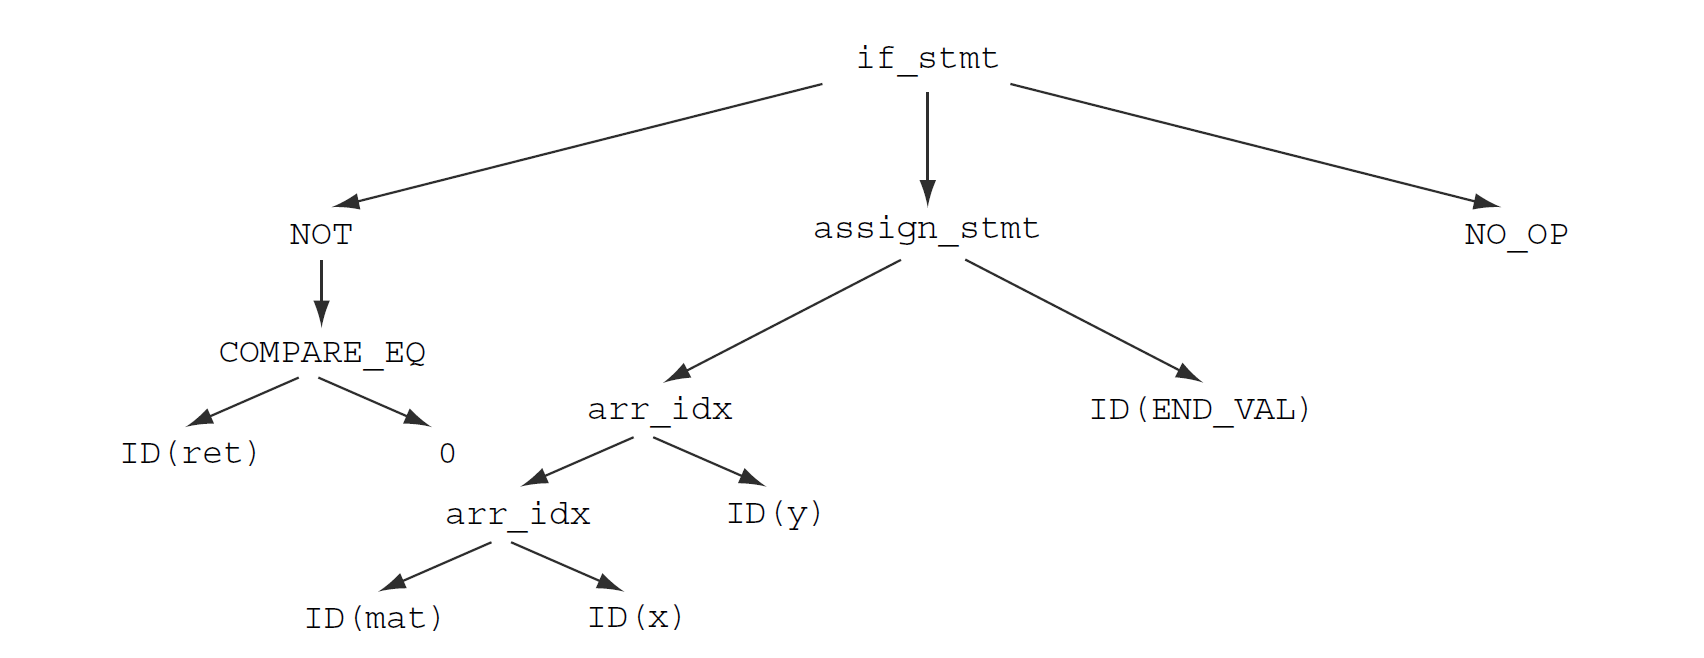
\includegraphics[width=1\textwidth]{Imagens/ArvoreAST}
		\label{fig:ArvoreAST}
		\caption{Árvore AST.}
	\end{figure}

	\section{Análise semântica}
	Como a AST está sendo construída, a ferramenta cria uma tabela de símbolos ao lado dela. Para cada identificador no programa, a tabela de símbolos associa o identificador com seu devido tipo e um ponteiro para a sua declaração ou definição. Com a AST e a tabela de símbolo, a ferramenta está agora equipado-se para realizar a verificação de tipo. A ferramenta de análise estática não pode ser obrigados a comunicar erros de checagem de tipo da maneira um compilador faz, mas informações de tipo é criticamente importante para a análise de uma linguagem orientada a objetos, porque o tipo de um objeto determina o conjunto de métodos que o objeto pode invocar. Além disso, é normalmente desejável para converter, pelo menos, as conversões do tipo implícito no código fonte para conversões de tipo explícitas no AST. Por estas razões, uma ferramenta de análise estática avançado tem a ver apenas como muito trabalho relacionado com a verificação de tipo como um compilador faz. No mundo do compilador, resolução de símbolo e verificação de tipo são referidos como análise semântica porque o compilador está atribuindo significado aos símbolos encontrada no programa. As ferramentas de análise estática que usam essas estruturas de dados têm uma vantagem distinta sobre ferramentas que não o fazem. Por exemplo, eles podem interpretar corretamente o significado dos operadores sobrecarregados em C++ ou determinar que um método em Java chamado doPost () é, na verdade, uma parte de uma implementação de HttpServlet.Estas capacidades permitem uma ferramenta para executar verificações úteis na estrutura deo programa. Após análise semântica, compiladores e a análise estática mais avançada ferramentas de formas de peça. Um compilador moderno usa a AST e o símbolo e o tipo informações para gerar uma representação intermediaria, uma versão genérico do código de máquina que é adequado para otimização e, em seguida, a conversão em específico da plataforma de código-objeto. O caminho para ferramentas de análise estática é menos clara. Dependendo do tipo de análise a ser realizada, uma ferramenta de análise estática pode executar transformações adicionais sobre a AST ou pode gerar a sua própria variedade de representação intermediária adequada às suas necessidades. Se uma ferramenta de análise estática usa sua própria representação intermediária, que, geralmente, permite a atribuição, pelo menos, ramificando, {\it looping}, e chamadas de função. A representação intermediária que uma ferramenta de análise estática usa é geralmente umvista de nível superior do programa do que a representação intermediária que um compilador usa. Por exemplo, um compilador de linguagem C, provavelmente, converter todas as referências a campos para estruturar deslocamentos em {\it byte} na estrutura pela sua representação intermediaria, enquanto uma ferramenta de análise estática mais provavelmente continuará para se referir a estrutura de campos, pelos seus nomes.

  \chapter{Suporte Ferramental para Minerar Padr\~{o}es de Uso de Constru\c c\~{o}es da Linguagem Java}

Com o intuito de obter uma compreens\~{a}o sobre o uso 
das constru\c c\~{o}es da linguagem Java, tornou-se 
necess\'{a}ria a implementa\c c\~{a}o de uma ferramenta 
de an\'{a}lise est\'{a}tica de prop\'{o}sito bem 
espec\'{i}fico, por outro lado com capacidade de 
ser extens\'{i}vel para extrair diferentes tipos de 
informa\c c\~{o}es. 
A Figura~\ref{fig:Arquitetura} apresenta 
uma vis\~{a}o geral dos elementos que comp\~{o}em o 
analisador est\'{a}tico desenvolvido durante a condu\c c\~{a}o 
deste trabalho de gradua\c c\~{a}o. Em linhas 
gerais, tal suporte ferramental recupera do sistema 
de arquivos todos os arquivos contendo código fonte 
escrito na linguagem Java, realiza o \textit{parse} 
desses arquivos gerando uma representação 
intermediária correspondente, mais adequada para 
as an\'{a}lises de interesse deste projeto, 
aplica uma série de mecanismos de análise estática 
para coletar as informações sobre o uso das 
caracter\'{i}sticas da linguagem de programa\c c\~{a}o e, por fim, 
gera os resultados no formato 
apropriado para as an\'{a}lises estat\'{i}sticas 
(no contexto deste projeto, foi feita a op\c c\~{a}o pelo 
formato CVS).

Atualmente existem diversas ferramentas e bibliotecas 
de programa\c c\~{a}o que auxiliam a constru\c c\~{a}o
de analisadores estáticos,  
conforme as nossas necessidades.
Entretanto, devido a maior experiência dos 
participantes do projeto com uso da linguagem Java, 
foi feita a op\c c\~{a}o por se utilizar a 
infraestrutura da plataforma \textit{Eclipse Java Development Tools}~\cite{EclipseJDT} 
(Eclipse JDT). O Eclipse JDT 
fornece um conjunto de ferramentas que auxiliam na constru\c c\~{a}o 
de ferramentas que permitem processar c\'{o}digo fonte escrito 
na linguagem de programa\c c\~{a}o Java. 
A plataforma Eclipse JDT é composta por 4 componentes principais: 
APT, Core, Debug e UI. Neste projeto a 
plataforma foi usada essencialmente através do \textit{JDT Core}, 
que dispõe de uma representa\c c\~{a}o Java 
para a navega\c c\~{a}o 
e manipula\c c\~{a}o dos elementos de uma árvore 
sintática~\acs{AST} gerada a partir do c\'{o}digo fonte, onde os elementos 
da representa\c c\~{a}o correspondem \`{a}s constru\c c\~{o}es 
sint\'{a}ticas da linguagem (como pacotes, classes, interfaces métodos e atributos). 

A~\acs{AST} provida pelo JDT é composta por 122 classes, 
como por exemplo existem 22 classe para representar senten\c cas  
como \textit{IF-Than-Else, Switch, While, BreakStatement} 
entre outras. Exitem cinco classes que trabalham exclusivamente com métodos referenciados 
e seis classes exclusivas que tratam os tipos declarados, como classes, interfaces 
e enumera\c c\~{o}es em Java.
O Eclipse JDT~\cite{EclipseJDT} disponibiliza ainda um \textit{parser} 
para a linguagem Java que atende a especifica\c c\~{a}o 
Java 8 da linguagem e que produz a representação intermediária baseada no conjunto de classes Java 
mencionado anteriormente e que corresponde 
a uma~\acs{AST} do código fonte. A plataforma tamb\'{e}m oferece 
uma hierarquia de classes 
para travessia na AST, de acordo com o padr\~{a}o de projeto \textit{visitor}~\cite{Gamma:1995}, e 
que facilita a análise estática 
de código fonte.

O padr\~{a}o de projeto \textit{Visitor}~\cite{Gamma:1995} \'{e} um 
padrão de projeto de característica comportamental que representa 
uma operação a ser realizada sobre elementos de uma \'{a}rvore de objetos. 
Neste caso, a operação a ser realizadas é visitar nós de interesse da AST Java 
(como os n\'{o}s que representam o uso de uma express\~{a}o Lambda em Java). 
Cada \textit{visitor} permite que uma nova operação seja criada 
sem que a estrutura da \'{a}rvore de objetos sofra alterações. Com isso, torna-se relativamente  
simples adicionar novas funcionalidades em um \textit{visitor} existente ou criar um novo \textit{visitor}.
Por outro lado, a biblioteca Eclipse JDT não fornece mecanismos para 
extração e exporta\c c\~{a}o de dados. Entretanto, no contexto 
deste projeto, foi implementado um conjunto de classes 
que visam obter maior facilidade e flexibilidade na exporta\c c\~{a}o das 
informa\c c\~{o}es coletadas durante a travessia nos n\'{o}s das 
ASTs. Essa flexibilidade foi alcançada com a utilização de introspecção de 
código que em Java é conhecido como \textit{reflection}. O 
restante desse cap\'{i}tulo apresenta mais detalhes sobre a arquitetura e 
implementa\c c\~{a}o do analisador est\'{a}tico, descrevendo 
as principais decis\~{o}es de projeto relacionadas \`{a}s cinco 
fases do analisador est\'{a}tico. 

\begin{figure}[tb]
	\center
	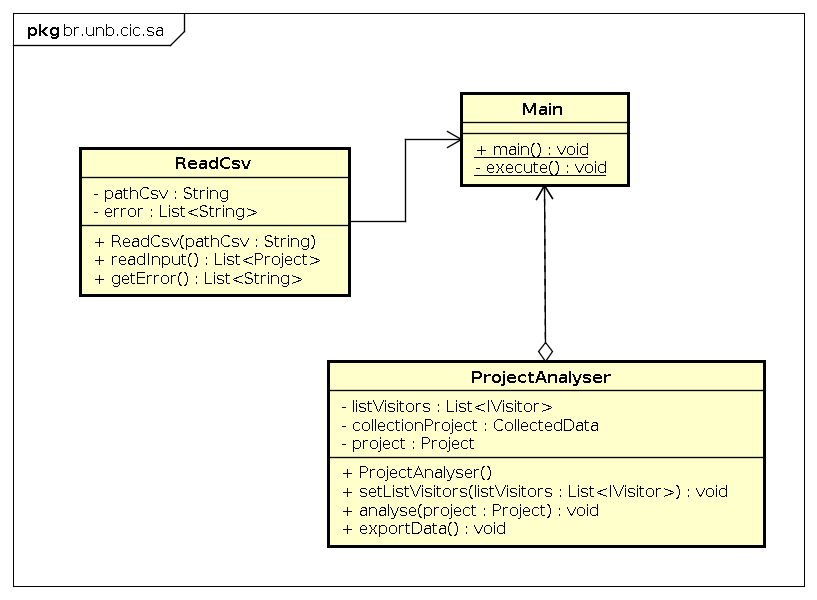
\includegraphics[scale=0.55]{Imagens/Arquitetura}
	\label{fig:Arquitetura}
	\caption{Vis\~{a}o geral da arquitetura do analisador est\'{a}tico}
\end{figure}


\section{Defini\c c\~{a}o dos Projetos a Serem Analisados}

O analisador estático recebe como entrada um arquivo \acs{CSV} (comma-separated values) 
que contém informa\c c\~{o}es sobre 
os projetos a serem analisados, como nome do projeto, 
caminho absoluto para uma pasta no sistema 
de arquivos contendo o c\'{o}digo fonte do projeto e a quantidade de linhas de código previamente 
computadas (conforme ilustrado na Figura:~\ref{fig:InputArquitetura}). 
As informações contidas no arquivo \acs{CSV} s\~{a}o processadas 
por um conjunto de classes utilitárias que percorrem os diretórios 
de um determinado projeto e seleciona todos os arquivos fonte da linguagem Java. 
Os códigos fontes Java encontrados servem ent\~{a}o como a entrada 
descrita na representa\c c\~{a}o abstrata 
do analisador est\'{a}tico (Figura:~\ref{fig:Arquitetura}). Ou seja, para cada 
projeto s\~{a}o recuperados os arquivos contendo 
c\'{o}digo fonte Java, que s\~{a}o convertidos para uma 
representa\c c\~{a}o intermedi\'{a}ria (por meio de 
um parser existente); processados e analisados com 
uma infraestrutura de \emph{visitors}, e os resultados das an\'{a}lises s\~{a}o ,por fim, 
exportados.

Conforme mencionado, essa fase do analisador est\'{a}tico realiza o processamento 
de cada arquivo Java dos projetos analisados. Sob a perspectiva de usabilidade, 
o usu\'{a}rio deve executar o programa principal informando, na linha de 
comando, o caminho para o arquivo \acs{CSV} contendo as defini\c c\~{o}es dos 
projetos. Isso produz uma lista contendo todos os projetos a serem processados 
(ver Linha 25 na Figura~\ref{fig:programaPrincipal}). Ap\'{o}s a lista de 
projetos ter sido carregada, cada projeto \'{e} analisado com o uso 
da classe \texttt{ProjectAnalyser}, que possui um m\'{e}todo 
(\texttt{analyse}) com a l\'{o}gica necess\'{a}ria para 
processar a base de c\'{o}digo fonte de cada projeto. A Figure~\ref{fig:metodoAnalyse} 
apresenta a implementa\c c\~{a}o do m\'{e}todo \texttt{analyse}, que 
recebe como par\^{a}metro um projeto. Note na linha seis da 
Figura~\ref{fig:metodoAnalyse} que o resultado do \textit{parse} 
em um arquivo fonte produz uma insta\^{a}ncia da classe 
\texttt{CompilationUnit} que pertence a plataforma 
Eclipse JDT e que representa a AST de um determinado 
arquivo Java. Essa classe possui um m\'{e}todo \texttt{accept}, 
conforme o padr\~{a}o de projeto \textit{visitor}, que \'{e} usado 
para pela ferramenta de an\'{a}lise est\'{a}tica para 
coletar as informa\c c\~{o}es do uso de constru\c c\~{o}es 
Java por meio de uma an\'{a}lise da representa\c c\~{a}o 
intermedi\'{a}ria. Isso \'{e} feito considerando cada um dos 
\emph{visitors} aplicados em uma an\'{a}lise espec\'{i}fica. 
  

\begin{figure}[htb]
\begin{lstlisting}
public class Main {
   
  public static void main(String[] args) {
    
    String pathCsv = ``''; 
    
    if(args.length == 1) {
      System.out.println(``Args: ''+ args[0].toString());
      pathCsv = args[0];
    }else {
      System.out.println(``Error: inform a valid csv file!!!\nEXIT'');
      System.exit(0);
    }
    
    ReadCsv rcsv = new ReadCsv(pathCsv);
    
    List<String> errors = rcsv.getError();
    
    errors.forEach(e -> System.out.println(``Error in '' + e));
 
    ApplicationContext ctx = CDI.Instance().getContextCdi(); 
    
    ProjectAnalyser pa = ctx.getBean(``pa'', ProjectAnalyser.class);
    
    List<Project> projects = rcsv.readInput();
    
    try {
      projects.stream().forEach(project -> pa.analyse(project));
    }catch(Exception t) {
      t.printStackTrace();
    }  
  }
}
\end{lstlisting}
  \caption{Classe que representa o programa principal do analisador est\'{a}tico}
  \label{fig:programaPrincipal}
\end{figure}


\begin{figure}[htb]
\begin{lstlisting}[language=Java]
public void analyse(Project p)  {
  CompilationUnit compilationUnit = null;
  List<String> fs = IO.list(p.getPath(), new String[] { ``java'' });
    
  for (String file : fs) {
    compilationUnit = Parser.Instance().parse(new File(file));
    
    for(IVisitor visitor : listVisitors){
      visitor.getCollectedData().setProject(p);
      visitor.setFile(file);
      visitor.setUnit(compilationUnit);
        
      compilationUnit.accept((ASTVisitor) visitor);
    }
  }    
  exportData();    
}
\end{lstlisting}
 \label{fig:metodoAnalyse}
 \caption{Implementa\c c\~{a}o do m\'{e}todo \texttt{analyse}, na classe \texttt{ProjectAnalyser}.}
\end{figure}

%% \begin{figure}[h]
%% 	\center
%% 	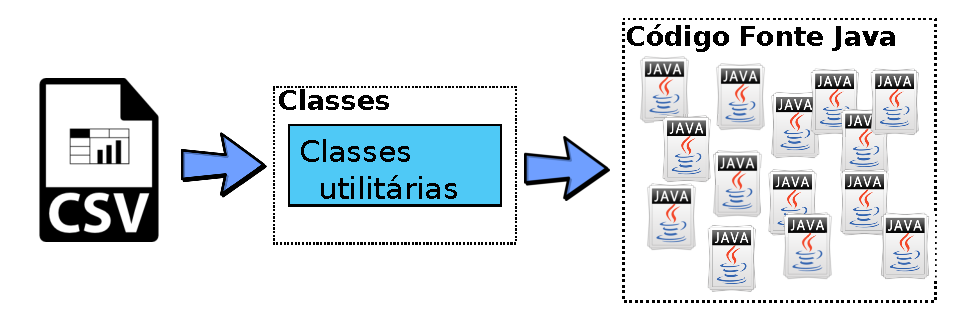
\includegraphics[scale=0.53]{Imagens/InputArquitetura}
%% 	\label{fig:InputArquitetura}
%% 	\caption{Input analisador estático.}
%% \end{figure}


\section{Análise da Representa\c c\~{a}o Intermedi\'{a}ria}

Conforme mencionado na se\c c\~{a}o anterior, o resultado do 
\textit{parser} em um arquivo fonte produz uma inst\^{a}ncia 
da classe \texttt{CompilationUnit}, que corresponde a 
uma AST com todas as defini\c c\~{o}es de tipo e 
implementa\c c\~{a}o de comportamento presentes em um m\'{o}dulo 
Java. A plataforma Eclipse JDT oferece uma infraestrutura 
de classes para realizar a traversia em uma AST, usando 
o padr\~{a}o de projeto \textit{visitor}. Dessa forma, 
foi feita uma implementa\c c\~{a}o de biblioteca de 
\textit{visitors}, para extrair as informa\c c\~{o}es 
presentes na representa\c c\~{a}o intermedi\'{a}ria.   

%% Após todos os código fontes Java identificado é dado início a verificação destes arquivos onde são processados e gerado um \textit{parser} para que os \textit{visitors} pesquisam padrões previamente estabelecidos onde a pesquisa elaborada com o principal objetivo de reconhecer elementos e sua subestruturas contidos no código fonte.
%% Com isso a representação intermediária deste analisador é o processamento do código fonte para convertê-lo em um \textit{parser} para que os  \textit{visitor} realizem sua pesquisa. A Figura:~\ref{fig:FuncionamentoAnalisador} demonstra o mais alto nível do funcionamento deste projeto.

%% \begin{figure}[h]
%% 	\center
%% 	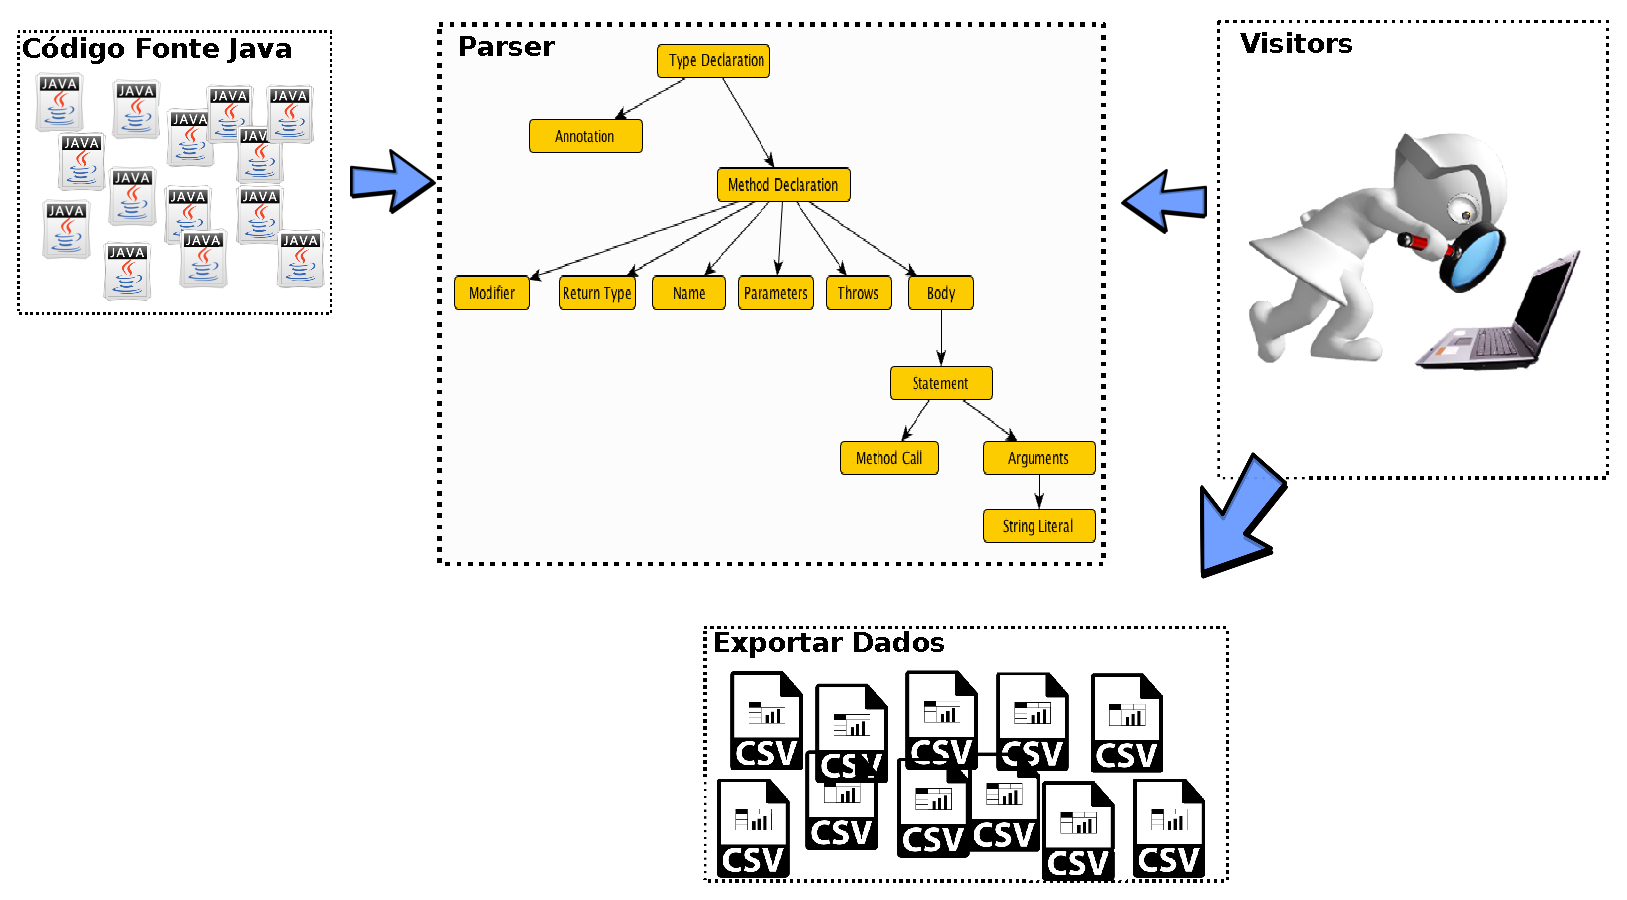
\includegraphics[scale=0.5]{Imagens/FuncionamentoVisitor}
%% 	\label{fig:FuncionamentoAnalisador}
%% 	\caption{Funcionamento analisador estático.}
%% \end{figure}

%{\color{red}{\bf rbonifacio}parece que ocorre uma transi\c c\~{a}o muito abrupta de uma discussão alto nivel para uma discussão muito rica em detalhes.}

% De forma mais técnica, a representa\c c\~{a}o intermedi\'{a}ria, para cada arquivo fonte o analisador
% est\'{a}tico realiza a coleta de dados utilizando uma infraestrutura de \textit{visitors}. 

No contexto deste projeto, 
e objetivando um maior grau de reuso, 
toda classe \emph{visitor} precisa herdar de uma classe abstrata e 
parametrizada em rela\c c\~{a}o a um tipo \texttt{T}, 
a classe \texttt{Visitor<T>}, 
onde o tipo \texttt{T} deve corresponder a classe usada para armazenar 
as informações coletadas pelo \emph{visitor}. O parâmetro de tipo \texttt{T} 
faz referência a uma 
classe composta basicamente por atributos e por 
opera\c c\~{o}es de acesso (\textit{getters} e \textit{setters}), 
que serve para representar os dados extraídos. 
Em geral, de acordo com a arquitetura do analisador est\'{a}tico proposto, 
para cada constru\c c\~{a}o que se 
deseja identificar o perfil de ado\c c\~{a}o nos projetos, s\~{a}o criadas 
duas classes: uma classe (\texttt{public class C\{ \ldots \}}) 
que representar as informa\c c\~{o}es de interesse 
associadas ao uso de uma constru\c c\~{a}o da 
linguagem Java e uma classe (\texttt{public class ConstVisitor extends Visitor<C> \{ \ldots \}}) 
que \emph{visita} a constru\c c\~{a}o de interesse na \'{a}rvore sint\'{a}tica abstrata. 
Por exemplo, a Figura~\ref{fig:enum} apresenta 
o c\'{o}digo necess\'{a}rio para visitar e popular informa\c c\~{o}es relacionadas a declara\c c\~{a}o de 
enumera\c c\~{o}es. A classe \texttt{public class Visitor<T> \{ \ldots \}} possui uma cole\c c\~{a}o 
de objetos do tipo parametrizado, sendo poss\'{i}vel adicionar inst\^{a}ncias desses objetos com a chamada 
\texttt{collectedData.addValue()}. Note que o exemplo apresentado corresponde a um dos mais simples 
\emph{visitors} implementados. Outros \emph{visitors} possuem uma l\'{o}gica mais elaborada, como por exemplo os 
\emph{visitors} que identificam oportunidades para usar constru\c c\~{o}es 
como \emph{multi-catch} ou \emph{lambda expressions}. 

\begin{figure}[htb]
\begin{lstlisting}
public class EnumDeclaration {
  private String file;
  private int startLine;
  private int endLine;
	
  //constructor + getters and setters.
}

public class EnumDeclarationVisitor extends Visitor<EnumDeclaration> {

  @Override
  public boolean visit(org.eclipse.jdt.core.dom.EnumDeclaration node) {
    
    EnumDeclaration dec = new EnumDeclaration(...);
		
    collectedData.addValue(dec);

    return true;
  }

}
\end{lstlisting}
\label{fig:enum}
\caption{Classes usadas para capturar declara\c c\~{o}es de enumera\c c\~{o}es.}
\end{figure}


%% O diagrama da Figura:~\ref*{fig:DiagramaVisitor} 
%% exibe de maneira técnica o procedimento de criar um \textit{Visitor} que detecte e colete informações dos tipos declarados no sistema, basta criar uma classes modelo \textit{TypeDeclaration.java} e  setar o parâmetro \textbf{<T>} como \textit{<TypeDeclaration>}, com isso os dados serão extraídas pelo \textit{Visitor, TypeDeclarationVisitor.java}, que identifica as informações pertinentes. {\color{red}refletir se esse par\'{a}grafo eh necessário}

%% \begin{figure}[h]
%% 	\center
%% 	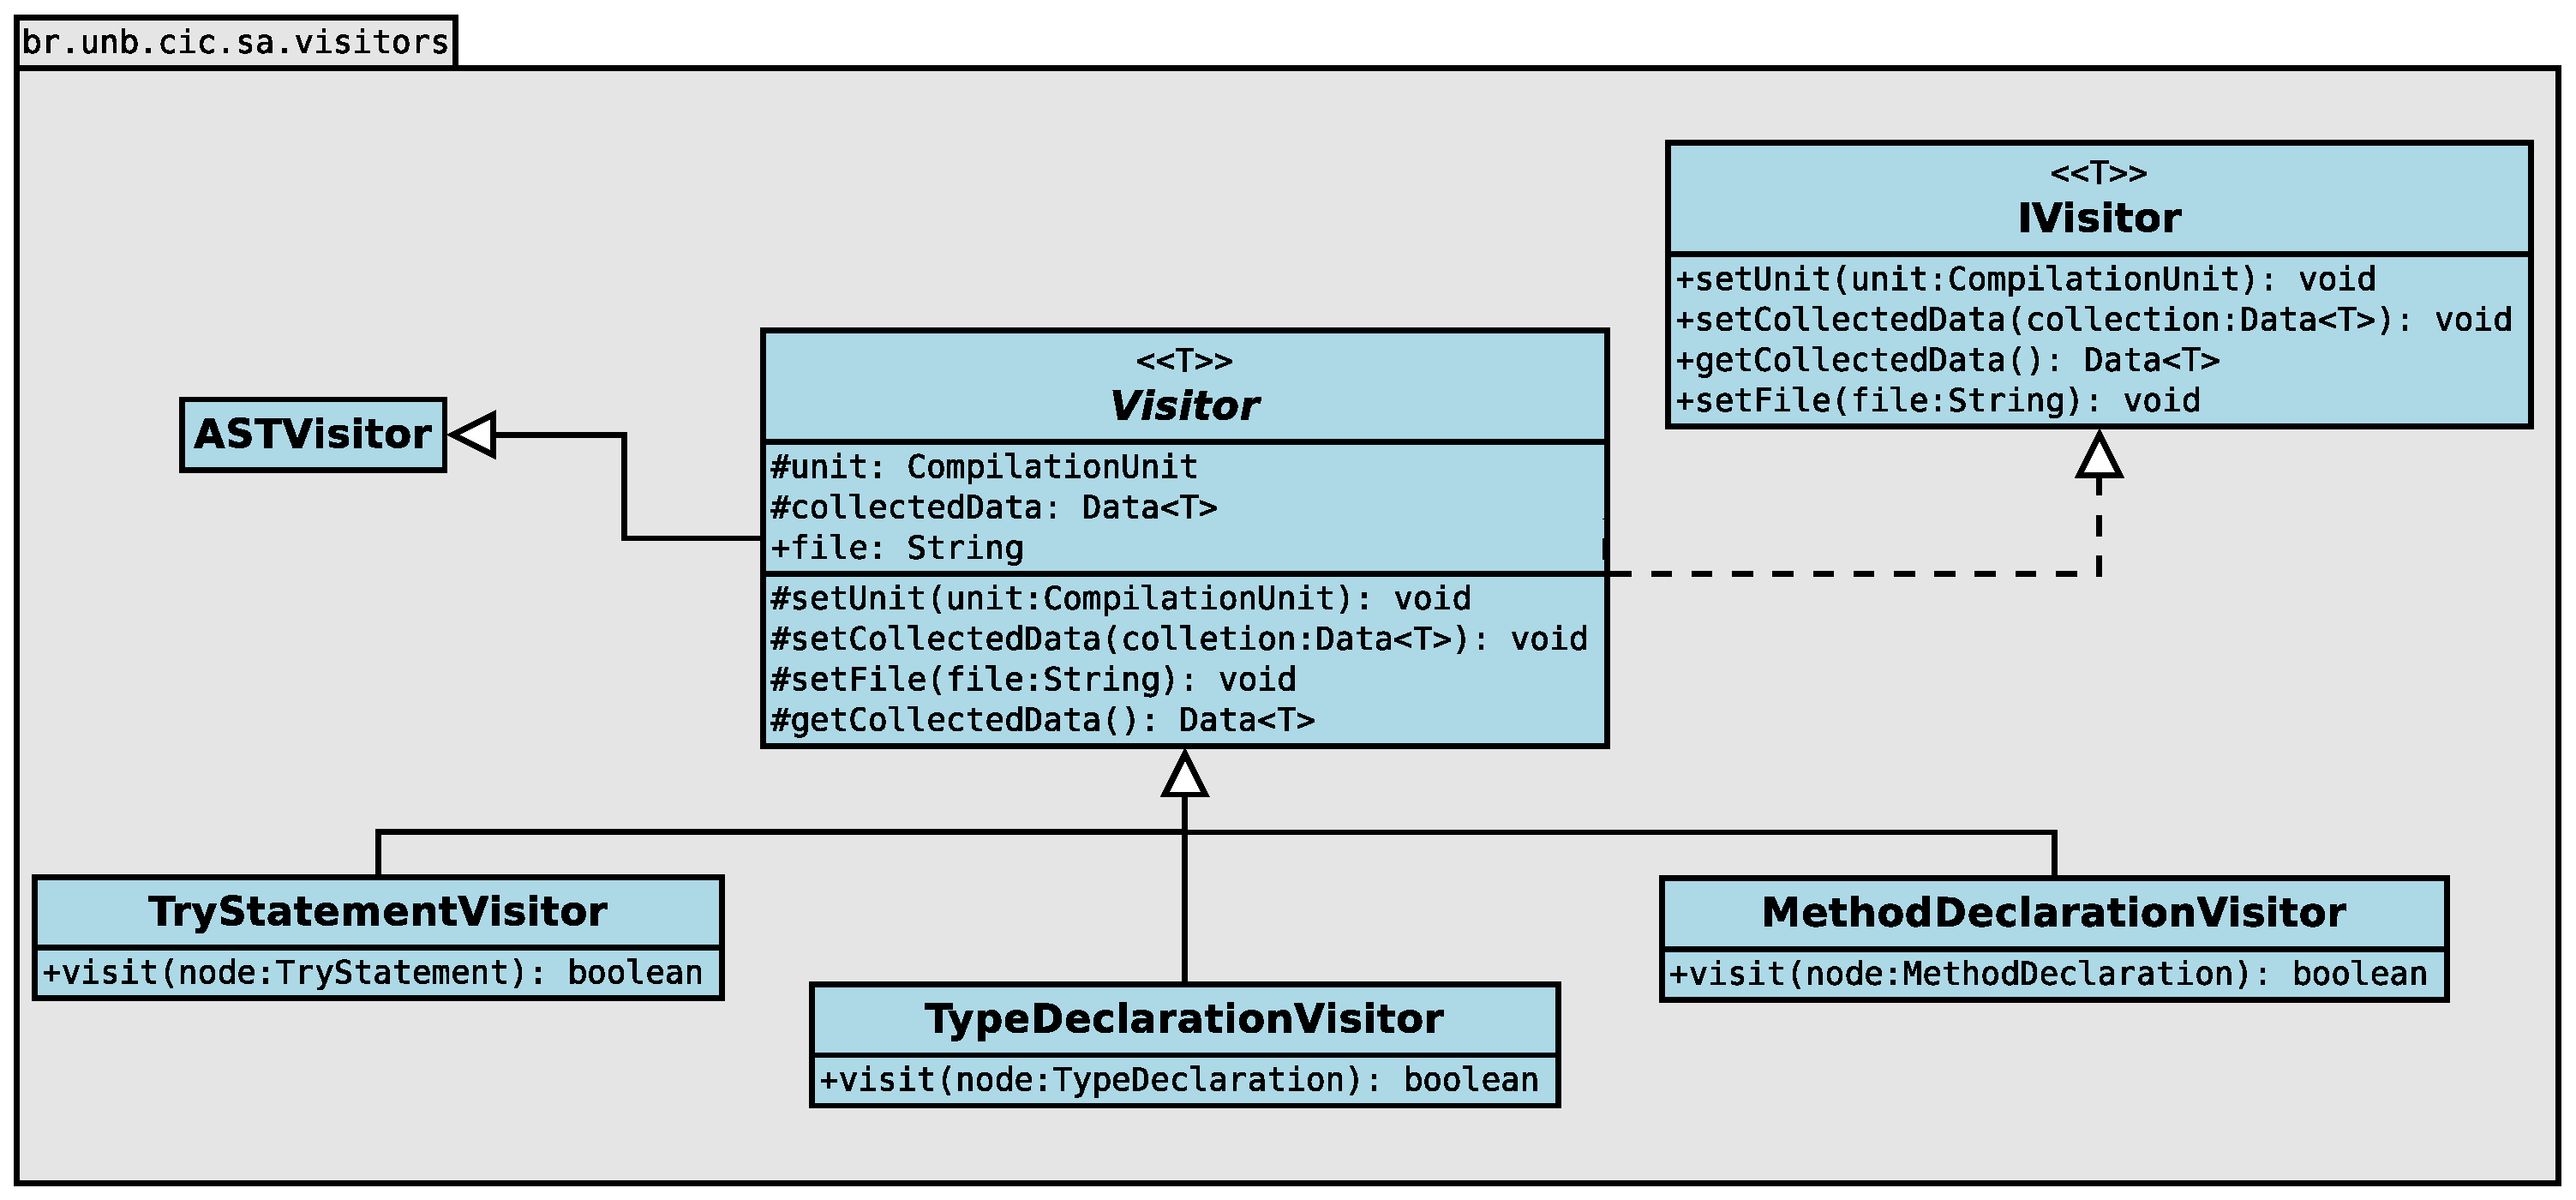
\includegraphics[scale=0.25]{Imagens/diagramaVisitor}
%% 	\label{fig:DiagramaVisitor}
%% 	\caption{Funcionamento analisador estático.}
%% \end{figure}

\subsection{Descri\c c\~{a}o dos Visitors}
Os \textit{visitors} implementados neste projeto 
s\~{a}o brevemente descritos a seguir, enquanto que 
a Tabela~\ref{tab:VisitorsCriados} apresenta 
duas m\'{e}tricas relacionadas \`{a} complexidade 
de implementa\c c\~{a}o, em termos de 
complexidade ciclom\'{a}tica e total de linhas de c\'{o}digo fonte. 
A complexidade ciclomática é dada pela quantidade de caminhos independentes 
em um trecho de código, enquanto que a quantidade de linhas de c\'{o}digo 
foi computada ignorando coment\'{a}rios e linhas em branco.  Vale 
ressaltar que a complexidade ciclom\'{a}tica 
dos \textit{visitors} varia entre um e oito  (com a média igual a 2.5). A 
quantidade média de linhas de código necessária para escrever um 
\textit{visitor} é 47.

\begin{itemize}
\item \texttt{AIC:} Coleta informa\c c\~{o}es relacionadas a declara\c c\~{a}o de 
\textit{Anonymous Inner Classes}. Tal informa\c c\~{a}o \'{e} \'{u}til 
para estimar oportunidades de uso de express\~{o}es lambda. 

\item \texttt{ExistPattern:} Coleta informa\c c\~{o}es de la\c cos \texttt{foreach} 
que iteram sobre uma cole\c c\~{a}o com o intuito de verificar se um 
determinado objeto est\'{a} presente na cole\c c\~{a}o. Tal informa\c c\~{a}o \'{e} \'{u}til 
para estimar oportunidades de uso de express\~{o}es lambda. 


\item \texttt{FieldAndVariableDeclaration:} Coleta informa\c c\~{o}es relacionadas 
a declara\c c\~{o}es de atributos e vari\'{a}veis, com o intuito de 
extrair informa\c c\~{o}es sobre a ado\c c\~{a}o de Java Generics. 

\item \texttt{FilterPattern:} Coleta informa\c c\~{o}es de la\c cos \texttt{foreach} 
que iteram sobre uma cole\c c\~{a}o com o intuito de 
filtrar elementos presentes na cole\c c\~{a}o. Tal informa\c c\~{a}o \'{e} \'{u}til 
para estimar oportunidades de uso de express\~{o}es lambda. 

\item \texttt{ImportDeclaration:} Coleta informa\c c\~{o}es relacionadas \`{a}
importa\c c\~{a}o de bibliotecas, sendo ]\'{u}til para estimar a ado\c c\~{a}o 
de bibliotecas voltadas para programa\c c\~{a}o concorrente ou integra\c c\~{a}o 
com linguagens de scripting, por exemplo. 

\item \texttt{LambdaExpression:} Coleta informa\c c\~{o}es relacionadas \`{a} 
ado\c c\~{a}o de express\~{o}es lambda. 

\item \texttt{Lock:} Verifica se os m\'{e}todos utilizam algum dos mecanismos 
de \emph{lock} suportados diretamente pela linguagem Java, como \texttt{Lock}, 
\texttt{ReentrantLock}, \texttt{ReadLock} ou \texttt{WriteLock}.

\item \texttt{MapPattern:} Coleta informa\c c\~{o}es de la\c cos \texttt{foreach} 
que iteram sobre uma cole\c c\~{a}o com o intuito de 
aplicar alguma opera\c c\~{a}o sobre os elementos presentes na cole\c c\~{a}o. 
Tal informa\c c\~{a}o \'{e} \'{u}til 
para estimar oportunidades de uso de express\~{o}es lambda. 

\item \texttt{MethodCall:} Coleta informa\c c\~{o}es relacionadas \`{a}s 
chamadas de m\'{e}todo, sendo \'{u}til para estimar o uso da API de 
introspec\c c\~{a}o de c\'{o}digo, por exemplo. 

\item \texttt{MethodDeclaration:} Coleta informa\c c\~{o}es relacionadas 
\`{a}s declara\c c\~{o}es de m\'{e}todos, sendo \'{u}til para identificar 
padr\~{o}es de uso de Java Generics, por exemplo.

\item \texttt{ScriptEngine:} Coleta informa\c c\~{o}es relacionadas 
ao uso da API Java para integra\c c\~{a}o com linguagens de scripting.  

\item \texttt{SwitchStatement:} Coleta informa\c c\~{o}es relacionadas 
ao uso de senten\c cas \texttt{switch-case}, com o intuito principal 
de identificar o uso de \texttt{strings} nesse tipo de senten\c ca. 

\item \texttt{SwitchString:} Coleta informa\c c\~{o}es associadas \`{a}s 
oportunidades de reestrutura\c c\~{a}o de c\'{o}digo para usar 
senten\c cas \texttt{switch-case} com \texttt{strings}. 

\item \texttt{TryStatement:} Coleta informa\c c\~{o}es relacionadas 
ao uso de blocos \texttt{try-catch}, em particular para estimar o 
uso da constru\c c\~{a}o \texttt{try-with-resources}. 

\item \texttt{TypeDeclaration:} Coleta informa\c c\~{o}es sobre 
os tipos declarados (classes, interfaces, enumera\c c\~{o}es), com 
o intuito, por exemplo, de estimar a ado\c c\~{a}o de Java Generics. 
\end{itemize}

\begin{table}[ht] \footnotesize
	\centering
	\caption{Estimativa da complexidade de desenvolvimento de cada \emph{visitor}.}
	\label{tab:VisitorsCriados}	
    \begin{tabular}{crr}
%		\begin{tabular}{M|p{9cm}}% centered column
			\hline 
			Visitor &  \acs{CC} & \acs{LoC}\\ \hline \hline
			
			\texttt{AIC} & 6 & 64\\ 
			
			\texttt{ExistPattern}  & 28 & 116\\ 
			
			\texttt{FieldAndVariableDeclaration} & 8 & 81\\ 
			
			\texttt{FilterPattern}  & 43 & 168\\ 
			
			\texttt{ImportDeclaration}& 1 & 63\\ 
			
			\texttt{LambdaExpression} & 1 & 33\\ 
			
			\texttt{Lock} & 12 & 75\\ 
			
			\texttt{MapPattern} & 27 & 103\\ 
			
			\texttt{MethodCall} & 2 & 22\\ 
			
			\texttt{MethodDeclaration} & 5 & 45\\ 
			
			\texttt{ScriptingEngine} & 5 & 39\\ 
			
			\texttt{SwitchStatement} & 3 & 35\\ 
			
			\texttt{SwitchStringOpportunities} & 3 & 50\\ 
		
			\texttt{TryStatement} & 11 & 80\\ 
			
			\texttt{TypeDeclaration} & 2 & 41\\ \hline
		\end{tabular}
\end{table}

% \section{Exporta\c c\~{a}o dos dados}

%% Para exportar os dados coletadas, foi constru\'{i}da uma solu\c c\~{a}o extens\'{i}vel, baseada no padr\~{a}o 
%% \emph{Inje\c c\~{a}o de Depend\^{e}ncia} e introspec\c c\~{a}o de c\'{o}digo. 
%% %\subsection{Injeçao de Dependência}


\subsection{Extensibilidade para Inclus\~{a}o de Novos Visitors}

Para tornar a solu\c c\~{a}o mais extens\'{i}vel, foram utilizados os mecanismos de 
\emph{Inje\c c\~{a}o de Depend\^{e}ncia} e introspec\c c\~{a}o de c\'{o}digo. 
Injeção de dependência \acs{DI}, \'{e} um mecanismo de extensibilidade mais 
conhecido como um padr\~{a}o de projeto originalmente denominado de inversão de controle (\acs{IoC}). 
De acordo com esse mecanismo, a sequência de criação dos objetos depende de como os mesmos são 
solicitados pelo sistema. Ou seja, quando um sistema é iniciado, 
os objetos necess\'{a}rios são instanciados e injetados de forma apropriada, 
geralmente de acordo com arquivo de configura\c c\~{o}es.
O mecanismo de inje\c c\~{a}o de depend\^{e}ncia foi incorporado na arquitetura 
com o uso do \textit{framework} Spring~\cite{SPRING_REF}, o que n\~{a}o causou 
nenhum impacto significativo na solu\c c\~{a}o inicialmente proposta e que n\~{a}o 
fazia uso de tal mecanismo--- os \emph{visitors} eram instanciados de maneira 
\emph{program\'{a}tica}. O uso do mecanismo de inje\c c\~{a}o de depend\^{e}ncia 
serviu para flexibilizar n\~{a}o apenas a incorpora\c c\~{a}o de novos \emph{visitors}, 
mas tamb\'{e}m para definir, de forma mais flex\'{i}vel, a estrat\'{e}gia de exporta\c c\~{a}o dos dados 
coletados. Gra\c cas ao mecanismo de inje\c c\~{a}o de depend\^{e}ncia, o desenvolvedor pode 
concentrar seu esforço na criação de \textit{visitors}, fazendo como que estes implementem a 
l\'{o}gica necess\'{a}ria para extrair as informações. Para que novos \emph{visitors} se conectem 
a plataforma, tornou-se necess\'{a}rio declarar o \textit{visitor} no arquivo com a defini\c c\~{a}o 
dos objetos gerenciados pelo Spring~\cite{SPRING_REF}. A 


\section{Exporta\c c\~{a}o dos Dados}

Na vers\~{a}o atual do suporte ferramental desenvolvido nessa monografia, os dados 
coletados pelo analisador est\'{a}tico s\~{a}o exportados exclusivamente no formato 
CSV. Esse formato facilita as an\'{a}lises estat\'{i}sticas usando o ambiente e linguagem 
de programa\c c\~{a}o R~\cite{R}. Também com foco na extensibilidade do sistema, os componentes envolvidos na 
geração de relatórios utilizam os mecanismos de inje\c c\~{a}o de depend\^{e}ncia, mencionado na 
se\c c\~{a}o anterior, e introspec\c c\~{a}o de c\'{o}digo, via a a API \textit{Reflection} da linguagem de 
programa\c c\~{a}o Java. Tal mecanismo oferece aos programadores a capacidade de escreverem componentes 
que podem observar e até modificar a estrutura e o comportamento dos objetos em tempo de execução.

A geração dos relatórios utiliza a classe \texttt{public class CSVData<T> \{ \ldots \ \}} onde o 
tipo parametrizado \texttt{<T>} é o mesmo utilizado para representar 
os dados coletados pelos \textit{visitors}. 
Os dados são obtidos através dos métodos de acesso (\textit{getters}) destas 
classes e exportados para arquivos~\acs{CSV}. 
O método \textit{export()} da classe \textbf{CSVData<T>} descobre quais dados s\~{a}o armazenados nos objetos do 
tipo \textbf{<T>}, usando o mecanismo de introspec\c c\~{a}o de c\'{o}digo. Com isso, \'{e} poss\'{i}vel 
generalizar a implementa\c c\~{a}o e simplificar a exporta\c c\~{a}o de dados coletados a partir de 
\textit{visitors} espec\'{i}ficos. Ou seja, após a descoberta dos dados coletados pelos \textit{visitors} usando 
introspec\c c\~{a}o, \'{e} poss\'{i}vel recuperar os mesmos assumindo a exist\^{e}ncia de m\'{e}todos de 
acesso (\textit{getters} de acordo com a especifica\c c\~{a}o Java Beans) e, 
como isso, export\'{a}-los em arquivos \acs{CSV} de saída. 
A Figura~\ref{fig:exportacao} apresenta o uso desse mecanismo para generalizar a exporta\c c\~{a}o dos 
dados. 

\begin{figure}
\begin{lstlisting}[language=Java]
public class CSVData<T> implements Data<T> {

  @Override
  public void export() {
    StringBuffer str = new StringBuffer("");
      
    if(data == null) { return; }
      
    for(T value : data) {
      //reflection code...
      for(Field f: value.getClass().getDeclaredFields()){
	  
	String fieldName = f.getName();
	String prefix = "get";
	  
	if(f.getType().isPrimitive() && f.getType().equals(Boolean.TYPE)) {
	  prefix = "is";
	}
					
	String methodName = prefix +
	Character.toUpperCase(fieldName.charAt(0)) +
	fieldName.substring(1);
	  
	Method m = value.getClass().getDeclaredMethod(methodName);						
	str.append(m.invoke(value));
	str.append(";");
	
	writer.append(str.toString());
	writer.append("\n");			
		
	writer.flush();  
      }
    }
  }
\end{lstlisting}
\label{fig:exportacao}
\caption{Exporta\c c\~{a}o de dados usando o mecanismo de introspec\c c\~{a}o de c\'{o}digo.}
\end{figure}

%Projetar um analisador estático para extrair informações de softwares desenvolvido não é uma simples tarefa, entretanto EclipseJDT~\cite{EclipseJDT} prove uma abstração significativa tornado menos árdua este projeto. O que pode possibilitar projetar uma arquitetura mais robusta para este analisador onde o foco de qualquer desenvolvedor que deseje utilizá-lo concentre-se apenas na produção de seus \textit{Visitors}. 
%
%Um ponto de extrema relevância foi tornar este analisador independente de qualquer plataforma e \acs{IDE} foi um ponto vital para o concepção deste projeto que não tem como intuito ser plugin de qualquer \acs{IDE} o que acarretaria na limitação do seu uso a um cenário específico mas sim uma ferramenta para apoiar no desenvolvimento de um software com construções atuais. Utilizando a portabilidade nativa entre as plataformas provido pela linguagem Java este trabalho foi concebido com intuito de atender ao mais diversos desenvolvedores quer utilizem Linux, Windows, Mac ou qualquer outro sistema operacional que tenha suporte para Java.
%
%A análise tem como início a seleção de projetos, nesse caso seleção em repositórios públicos, onde após o download é informado analisador o diretório raiz onde estes estão localizados. Após é iniciado uma listagem dos arquivos fonte Java contidos nos projeto e contabilizados o total de \acs{LOC} e criado uma árvore sintática para cada arquivo encontrado através de um \textit{parser} provido pela biblioteca EclipseJDT~\cite{EclipseJDT}. Em seguida os \textit{Visitors} são instanciados com o objetivo de percorrer os nós destas árvores para pesquisar por construções de código previamente determinadas.
%
%Todas as construções pesquisadas quando encontradas pelos \textit{Visitors} são armazenadas temporariamente enquanto o analisador verifica todo projeto, quando é verificado a última árvore sintática pelos \textit{Visitors} é iniciado o processo de exportar os dados encontrados para um arquivo \acs{CSV} o conteúdo relevante destes blocos, a Figura:~\ref{fig:Arquitetura} demostra de maneira clara o funcionamento do analisador. Após a exportação dos dados o analisador inicia todo processo novamente caso exista mais de um projeto.
%
%Devido ao mecanismo de \textit{reflection} proveniente da linguagem Java, o desenvolvedor não tem a necessidade de implementar código para exportação de dados tendo em vista que isto ocorre automaticamente através da introspecção realizada pelo analisador extraindo os dados armazenados pelos \textit{Visitors}.

%	\begin{figure}[h]
%		\center
%		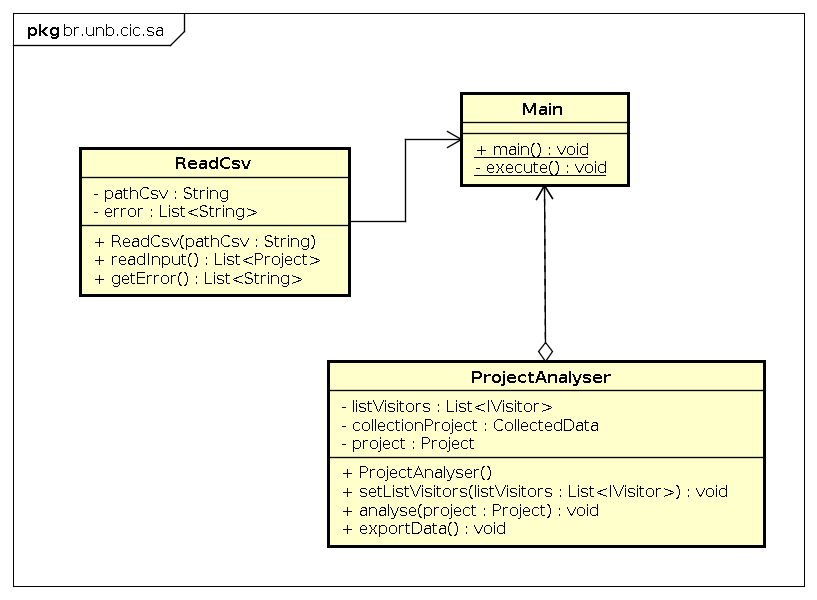
\includegraphics[scale=0.52]{Imagens/Arquitetura}
%		\label{fig:Arquitetura}
%		\caption{Funcionamento analisador estático.}
%	\end{figure}


%\section{Arquitetura}
%
%\subsection{Visitors}
%
%
%
%\begin{lstlisting}
%package br.unb.cic.sa.visitors;
%
%import org.eclipse.jdt.core.dom.ASTVisitor;
%import org.eclipse.jdt.core.dom.CompilationUnit;
%import br.unb.cic.sa.model.Data;
%
%public class Visitor<T> extends ASTVisitor implements IVisitor<T> {
%	protected CompilationUnit unit;
%	protected Data<T> collectedData;
%	protected String file;
%	
%	public Visitor() {}
%	
%	@Override
%	public void setUnit(CompilationUnit unit) { this.unit = unit; }
%	
%	@Override
%	public void setCollectedData(Data<T> colletion) { this.collectedData = colletion; }
%	
%	@Override
%	public void setFile(String file) {	this.file = file; }
%
%	@Override
%	public Data<T> getCollectedData() {	return collectedData;	}	
%}
%\end{lstlisting}
%
%
%A tabela:~\ref{tab:VisitorsCriados} detalha os 17 \textit{Visitors} criados com a respectiva descrição do trabalho realizado. Como forma de exemplificar a criação de um \textit{Visitors}, etapa a qual é composta de 4 passos quo serão demonstrados a seguir.
%
%A investigação para saber como o tratamento de exceção Java tem sido utilizado acarretou na criação de um \textit{Visitor} específico para este fim, \textit{TryStatementVisitor}, responsável por pesquisar este mecanismo o qual pode contar com alguma evoluções ao logo do histórico da linguagem Java. A pesquisa é iniciada encontrando blocos \textit{trys/catch}, onde destes será coletadas as informações referentes a adoção de \textit{resources} e oportunidade de utilizar \textit{multicatch} em blocos \textit{trys} que contenham \textit{catchs} iguais aninhados.
%%, neste caso de oportunidades os \textit{catchs} são testados por igualdade mas é trivial a utilização de um algoritmo mais avançado que teste a similaridade.
%
%Criação do \textit{Visitor TryStatementVisitor} com exemplo.
%
%	\begin{enumerate}
%		\item Inicialmente é necessário criar a classe modelo onde esta terá atribuição de receber os dados que serão extraídos pelos \textit{Visitors}, basicamente as classes modelos são compostas de \textit{getters} e \textit{setters} e são declaradas no pacote  \textit{\textbf{br.unb.cic.sa.model}}.
%			\begin{lstlisting}
%package br.unb.cic.sa.model;
%
%public class TryStatementData  {
%	private String file;
%	private int startLine;
%	private int endLine;
%	private boolean tryWithResource = false;
%	private boolean multiCatch = false;
%	
%	public TryStatementData(String file, int startLine, int endLine){
%		this.file = file;
%		this.startLine = startLine;
%		this.endLine = endLine;
%	}
%	
%	//getters and setters
%}
%			\end{lstlisting}
%			
%			
%		\item Em seguida, é concebida a criação do \textit{Visitor} no pacote \textit{\textbf{br.unb.cic.sa.visitors}} onde esta nova classe será estendida da classe parametrizada \textit{\textbf{Visitor<TryStatementData>}} apresentada anteriormente onde a parametrização desta classe é o modelo criado anteriormente.
%			
%			\begin{lstlisting}
%package br.unb.cic.sa.visitors;
%
%import java.util.List;
%import org.eclipse.jdt.core.dom.CatchClause;
%import org.eclipse.jdt.core.dom.TryStatement;
%import br.unb.cic.sa.model.TryStatementData;
%import br.unb.cic.sa.similarity.BasicSimilarityChecker;
%import br.unb.cic.sa.similarity.SimilarityChecker;
%
%public class TryStatementVisitor extends Visitor<TryStatementData> {
%
%	SimilarityChecker similarity;
%
%	public TryStatementVisitor() {
%		similarity = new BasicSimilarityChecker();
%	}
%
%	@Override
%	public boolean visit(s node) {
%
%		TryStatementData t = new TryStatementData(this.file, unit.getLineNumber(node.getStartPosition()),
%				unit.getLineNumber(node.getStartPosition() + node.getLength()));
%		
%		if (node.resources().size() > 0) {
%			t.setTryWithResource(true);
%		}
%	
%		if (node.catchClauses().size() > 1) {
%			if (this.checkSimilarity(node.catchClauses())) {
%				t.setMultiCatch(true);
%			}
%		}
%
%		this.collectedData.addValue(t);
%
%		return super.visit(node);
%	}
%	
%	private boolean checkSimilarity(List<CatchClause> catchClause) {
%		for (CatchClause cc : catchClause) {
%			for (CatchClause cn : catchClause) {
%				// To ignore the same catch in loops
%				if (!cc.equals(cn)) {
%				
%				//Chamada externa para testar similaridade
%					if (this.similarity.checkSimilarity(cc.getBody(),
%														cn.getBody())) {
%						return true;
%					}
%				}
%			}
%		}
%		return false;
%	}
%
%}
%			\end{lstlisting}
%			
%		 Na linha24, é testada a condição para saber se este bloco fez adoção de \textit{Resouce}. Na linha 30 é verificado que o bloco é um possível caso de \textit{multicatch} pois existe mais de um bloco. Na linha 39 tem-se o método \textit{checkSimilarity} o qual efetua a comparação dos blocos \textit{Catch} aninhados, entretando de forma trivial na linha 46, pode ser utilizado um algoritmo mais sofisticado para testar por similaridade modificando apenas o conteúdo do método \textbf{\textit{checkSimilarity}} da classe \textit{\textbf{SimilarityChecker}} o que não resulta em mudanças neste \textit{Visitor}.
%		
%	
%			\item Em seguida deve-se declarar o cabeçalho no arquivo \textit{resource/Beans.xml} do \textit{Spring} que estará presente no \acs{CSV} de saída. Onde este cabeçalho é composto pelo dados que serão extraídos pelos \textit{Visitors} e armazenados no modelo criado.
%			
%			\begin{lstlisting}
%<bean id="tryStatementData" class="br.unb.cic.sa.model.CSVData">
%	<property name="outDir" value="output"/>
%	<property name="fileName" value="tryStatement"/>
%	<property name="head" value="typeProject, before, project, version, file, start, end, resource, multiCatch"/> 
%</bean>
%			\end{lstlisting}
%			
%			
%			\item Por fim declarar o \textit{Visitor} como um \textit{bean} do \textit{Spring} para que este seja injetado no projeto e assim realize sua pesquisa.
%			
%			\begin{lstlisting}
%<bean id="tryStatementVisitor" class="br.unb.cic.sa.visitors.TryStatementVisitor">
%	<property name="collectedData" ref="tryStatementData"/>
%</bean>
%			\end{lstlisting}
%			
%	\end{enumerate}
%
%
%
%\subsection{Exportar Dados}
%A exportação dos dados para \acs{CSV} é realizado de forma automática utilizando o mecanismo de \textit{reflection} fornecido por Java. A classe parametrizada \textbf{\textit{CSVData<T>}} no pacote \textbf{\textit{br.unb.cic.sa.model}} implementa a interface \textit{\textbf{Data<T>}} onde \textbf{\textit{<T>}} faz  aos modelos declarados para as informações coletadas.
%
%\begin{lstlisting}
%package br.unb.cic.sa.model;
%
%public interface Data<T> {
%	public void setProject(Project project);
%	public void addValue(T value);
%	public void export();
%	public int size();
%	public void clean();
%}
%\end{lstlisting}
%
%
%Onde o atributo \textit{String[] head} é injetado pelo \textit{Spring} pois fora declarado anteriormente na criação do visitor. O método \textbf\textit{{export()}}, na linha 23, é o método responsável para exportar os dados em seus respectivos \acs{CSV} pois este método recupera as informações contidas nas coleções populadas pelos \textit{Visitors} e com \textit{reflection} captura os campos declarados em especial para os métodos quais são pré-fixados com \textit{get ou is} que terão seus valores capturados para que sejam exportados.
%
%\begin{lstlisting}
%package br.unb.cic.sa.model;
%
%import java.io.File;
%import java.io.FileWriter;
%import java.io.IOException;
%import java.lang.reflect.Field;
%import java.lang.reflect.InvocationTargetException;
%import java.lang.reflect.Method;
%import java.util.ArrayList;
%import java.util.List;
%
%public class CSVData<T> implements Data<T>{
%
%	private Project project;
%	private String fileName;
%	private String outDir;
%	private String[] head; 
%	private List<T> data;
%
%	...
%	
%	@Override
%	public void export() {
%		
%		try (FileWriter writer = new FileWriter(this.makeCsv(head), true)){
%		
%			StringBuffer str = new StringBuffer("");
%
%			if(data == null) {
%				return;
%			}
%			
%			for(T value : data) {
%				str = new StringBuffer("");
%				
%				str.append(project.getTypeOfProject());
%				str.append(";");
%				str.append(project.getBefore());
%				str.append(";");
%				str.append(project.getProjectName());
%				str.append(";");
%				str.append(project.getProjectRevision());
%				str.append(";");
%			
%				for(Field f: value.getClass().getDeclaredFields()){
%										
%					String fieldName = f.getName();
%					String prefix = "get";
%					
%					if(f.getType().isPrimitive() &&
%					   f.getType().equals(Boolean.TYPE)) {
%						prefix = "is";
%					}
%					
%					String methodName = prefix + 
%								Character.toUpperCase(fieldName.charAt(0)) +
%								fieldName.substring(1);
%										
%					try {
%						Method m = value.getClass().getDeclaredMethod(methodName);						
%						str.append(m.invoke(value));
%						str.append(";");
%					}catch(
%							NoSuchMethodException | 
%							IllegalAccessException |
%							IllegalArgumentException |
%							InvocationTargetException e) {
%							
%						throw new RuntimeException("Type " + 
%											value.getClass().getName() +
%											" must have a method named " +
%											 methodName);
%					}
%				}
%				
%				writer.append(str.toString());
%				writer.append("\n");
%				
%			}
%		
%			writer.flush();
%		
%		}
%		catch(Exception e) {
%			e.printStackTrace();
%		}
%	}
%}
%
%\end{lstlisting}

  \chapter{Resultados}
\section{Lambda}
Ao todo o visitor responsável por pesquisar a adoção de \textit{Lambda} encontrou somente 814 caso de uso. Distribuidos em 354 arquivos o que leva a acreditar que tal característica não esta sendo tão relevante quanto sua espectativa de lançamento. Onde somente 2 casos não estão envolvidos em testes unitátos, os demais 812 estão sendo empregados no desevolvimento de testes unitários conforme exibido pela figura: \ref{fig:AdocaoLambda}. Vale resaltar que somente duas únicas ocorrências de lambda foram encontradas no projeto Jetty versão 9.3.2 nos fontes \textit{PathMap.java} e \textit{RegexSet.java}.\\

\begin{figure}[h]
	\center
	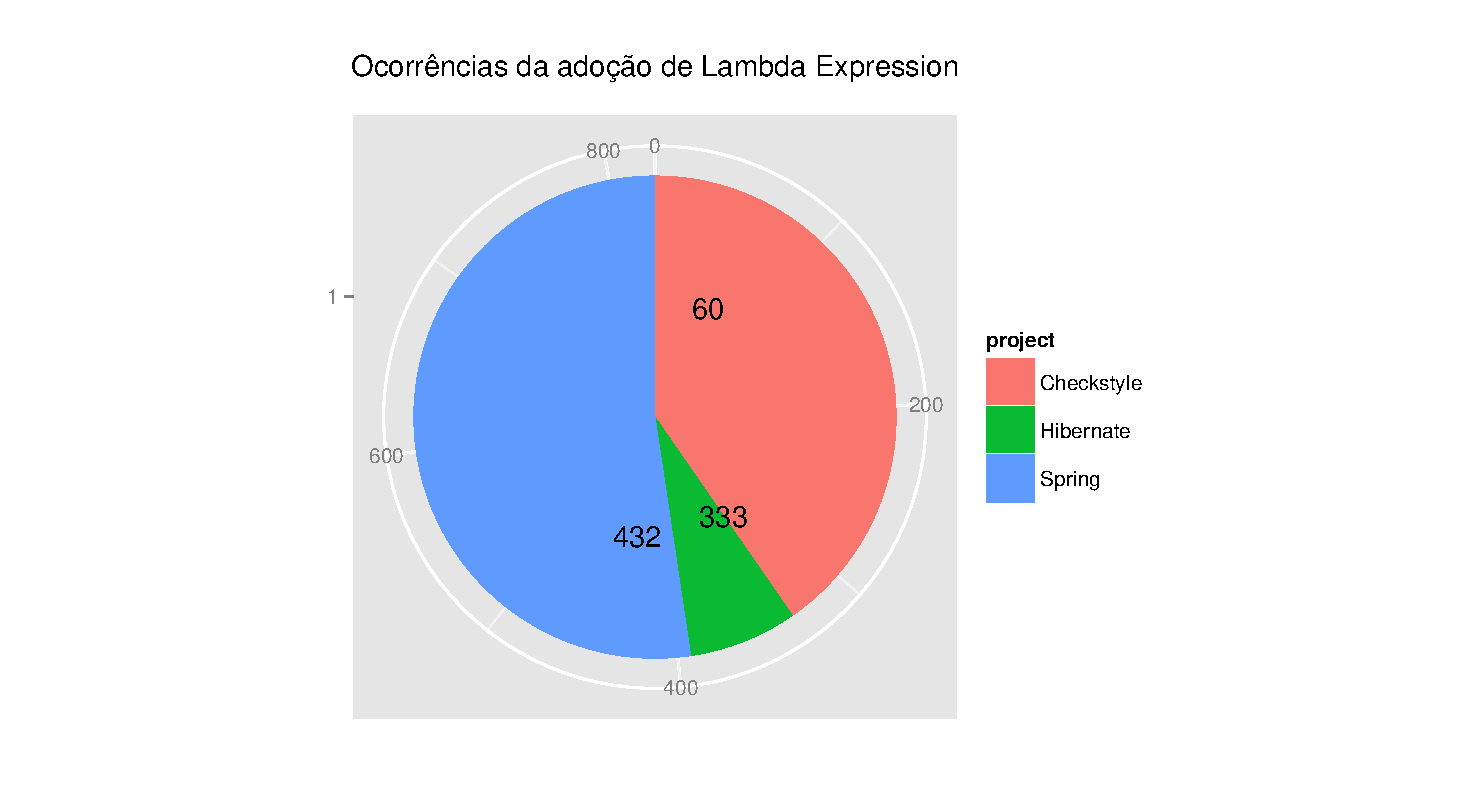
\includegraphics[scale=0.8]{Imagens/AdocaoLambdaTestes}
	\label{fig:AdocaoLambda}
	\caption{Adoção de \textit{Lambda} em testes unitários.}
\end{figure}



\subsection{Oportunidades de Aplicar Lambda}
Entretanto foram encontradas XXXXX oportunidades de converter \textit{For} que iteram \textit{Collections} para \textit{Lambda} através da \textit{Inteface Stream}, totalizando XXX \acs{LOC}. Estas esão dividida confome a figura: \ref{OpportunidadesLambda}.\\

\subsection{Oportunidades para uso da constru\c c\~{a}o \texttt{multi-catch}}

O uso da constru\c c\~{a}o \texttt{multi-catch} permite reduzir qualquer 
l\'{o}gica duplicada existente em blocos \texttt{catch} distintos de 
uma contru\c c\~{a}o \texttt{try-catch}. Com as an\'{a}lises realizadas, 
foi poss\'{i}vel identificar uma quantidade significativa de oportunidades 
de uso dessa constru\c c\~{a}o, conforme exibido na Figura: \ref{fig:Muticatch}. Ao todo, 
foram encotrados \num{10368} blocos \texttt{try} que possuem \textit{catchs} repetidos. 
Essas ocorrências estão distribuídas em \num{7297} arquivos e totalizamo \num{97347} \acs{LOC}. 
Importante observar que o teste de  similaridade entre os blocos \texttt{catch} 
foi realizado através de uma chamada a um método exteno que verificava a igualdade da \'{a}rvore 
sint\'{a}tica. Apesar dessa abordagem n\~{a}o fazer uso de uma estrat\'{e}gia de an\'{a}lise 
de similaridade de c\'{o}digo mais robusta, a mesma pode ser facilmente alterada de 
acordo com algum algoritmo existente. 


\begin{figure}[h]
	\center
	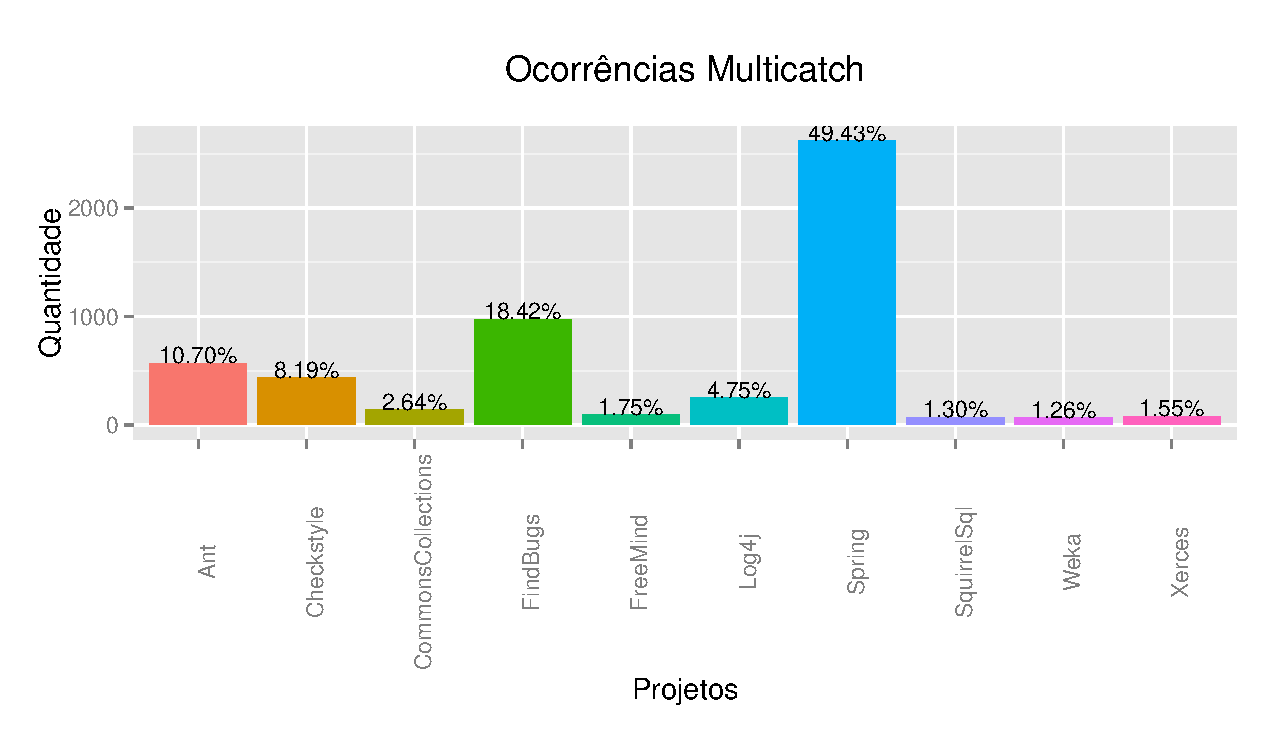
\includegraphics[width=13cm,height=7.8cm]{Imagens/ocorrenciasMulticatch}
	\label{fig:Muticatch}
	\caption{Oportunidades de \textit{Multicatch} nos projetos.}
\end{figure}
		

Considere os exemplos nas listagens {\color{red} X e Y}, 
encontrados na classe \texttt{AbstractNestablePropertyAccessor} do projeto \textit{Spring 4.2.0.RC2}. 
Neste caso, é possível reestruturar o c\'{o}digo para usar a constru\c c\~{a}o 
\texttt{multi-catch}, o que levaria a uma redu\c c\~{a}o de {\color{red} 40\%}  para 
esse trecho de código. Um simples \textit{refactoring} unindo todos os blocos 
que potencialmente se beneficiariam do uso de blocos \texttt{multi-catch} levaria a uma redução de 
68063 \acs{LOC}, tornando essa constru\c c\~{a}o  \'{u}til para reduzir a quantidade de 
linhas de c\'{o}digo em duplicidade de um projeto. 
\begin{lstlisting}[]
// Sem uso de Multicacth 17 LOC
try {...}
catch (ConverterNotFoundException ex) {
  PropertyChangeEvent pce = new PropertyChangeEvent(this.rootObject, this.nestedPath + propertyName, oldValue, newValue);
  throw new ConversionNotSupportedException(pce, td.getType(), ex);
}catch (ConversionException ex) {
  PropertyChangeEvent pce = new PropertyChangeEvent(this.rootObject, this.nestedPath + propertyName, oldValue, newValue);
  throw new TypeMismatchException(pce, requiredType, ex);
}catch (IllegalStateException ex) {
  PropertyChangeEvent pce = new PropertyChangeEvent(this.rootObject, this.nestedPath + propertyName, oldValue, newValue);
  throw new ConversionNotSupportedException(pce, requiredType, ex);
}catch (IllegalArgumentException ex) {
  PropertyChangeEvent pce = new PropertyChangeEvent(this.rootObject, this.nestedPath + propertyName, oldValue, newValue);
  throw new TypeMismatchException(pce, requiredType, ex);
}
\end{lstlisting}


\begin{lstlisting}
 //  Com uso de Multicatch 10 LOC
 try {...}
 catch (ConverterNotFoundException ex | IllegalStateException ex) {
   PropertyChangeEvent pce = new PropertyChangeEvent(this.rootObject, this.nestedPath + propertyName, oldValue, newValue);
   throw new ConversionNotSupportedException(pce, td.getType(), ex);
 }catch (ConversionException ex | IllegalArgumentException ex) {
   PropertyChangeEvent pce = new PropertyChangeEvent(this.rootObject, this.nestedPath + propertyName, oldValue, newValue);
   throw new TypeMismatchException(pce, requiredType, ex);
 }	
\end{lstlisting}

%Uma análise mais detalhada sobre \textit{JBoss, Spring, Hibernate e Findbugs} totalizando juntos 7778 ocorrências, iniciando na 3.0.0.M1 lançada em junho de 2009 até a mais recente até o momento 4.2.0.RC2. Para uma análise mais criteriosa será elaborada um detalhamento a partir da versão 4.0.0.M1 até a 4.2.0.RC2 totalizando 927 oportunidades de \textit{multicatch} 35\% das ocorrências no \textit{Spring}.\\

A figura: \ref{fig:ocorrenciasMulticatchVersoes} exibe as ocorrências nos projetos mais numerosos do estudo. Onde todas as ocorrências totalizam 17100 \acs{LOC} e após um simples \textit{refactoring}, 
conforme o exemplo anterior, obtem-se 5955 \acs{LOC} o que acarreta uma redução da ordem de 65\% de c\'{o}digo duplicado em blocos \texttt{catch}.

\begin{figure}[h]
	\center
	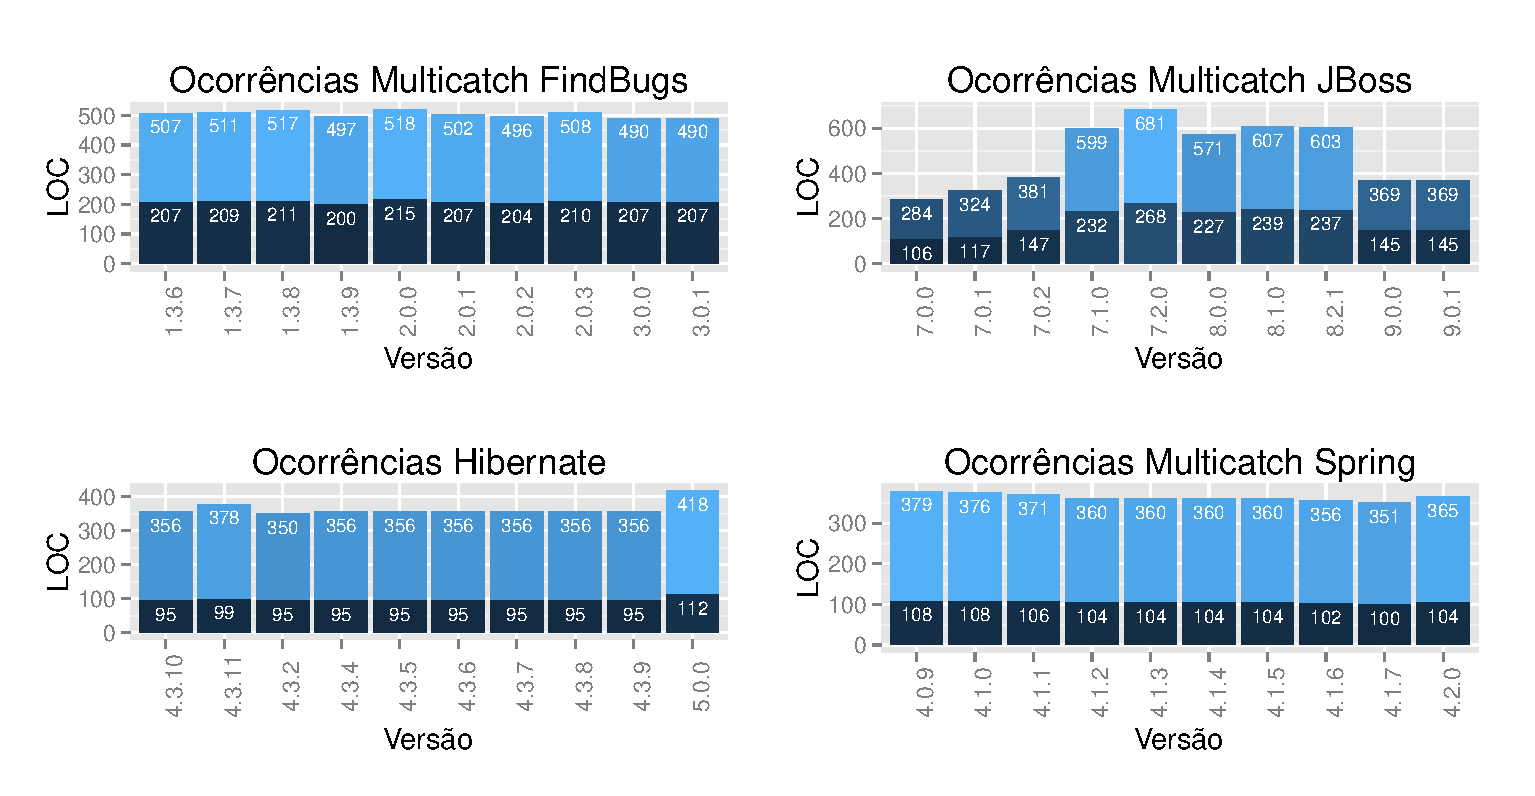
\includegraphics[height=8cm, keepaspectratio]{Imagens/ocorrenciasMulticatchVersoes}
	\label{fig:ocorrenciasMulticatchVersoes}
	\caption{Oportunidades de \textit{Multicatch} nos projetos.}
\end{figure}


\section{Try Resource}
O visitor responsável por detectar a adoção desta \textit{feature} pesquisou por padrões como o código abaixo onde não foi pesquisado oportunidades de \textit{refactoring} mas sim onde esta característica estava sendo adotada.
\begin{lstlisting}
static String readFirstLineFromFile(String path) throws IOException {
	try (BufferedReader br = new BufferedReader(new FileReader(path))) {
		return br.readLine();
	}
}
\end{lstlisting}

Com o advento do Java 7 foi introduzido o \textit{Try with Resource} onde um \textit{resource} é um objeto que pode ser fechado antes do programa ser encerrado. Com isso promoveu uma maior autonomia e flexibilidade ao programador. Foi encontrado no total 284321 \textit{trys} nos quais  esta \textit{feature} totaliza 1.8\%, ou seja, 5186 casos. Conforme exibido na figura: ~\ref{fig:Try with Resource} exibe a distribuição desta \textit{feature} entre os projetos onde pode-se constatar que somente 4 projetos fizera a adoção. Com exceção do projeto \textit{Jetty} que totaliza 87\% dos casos os demais projetos não aderiram de forma massiva esta caracterísitica.


\begin{figure}[h]
	\center
	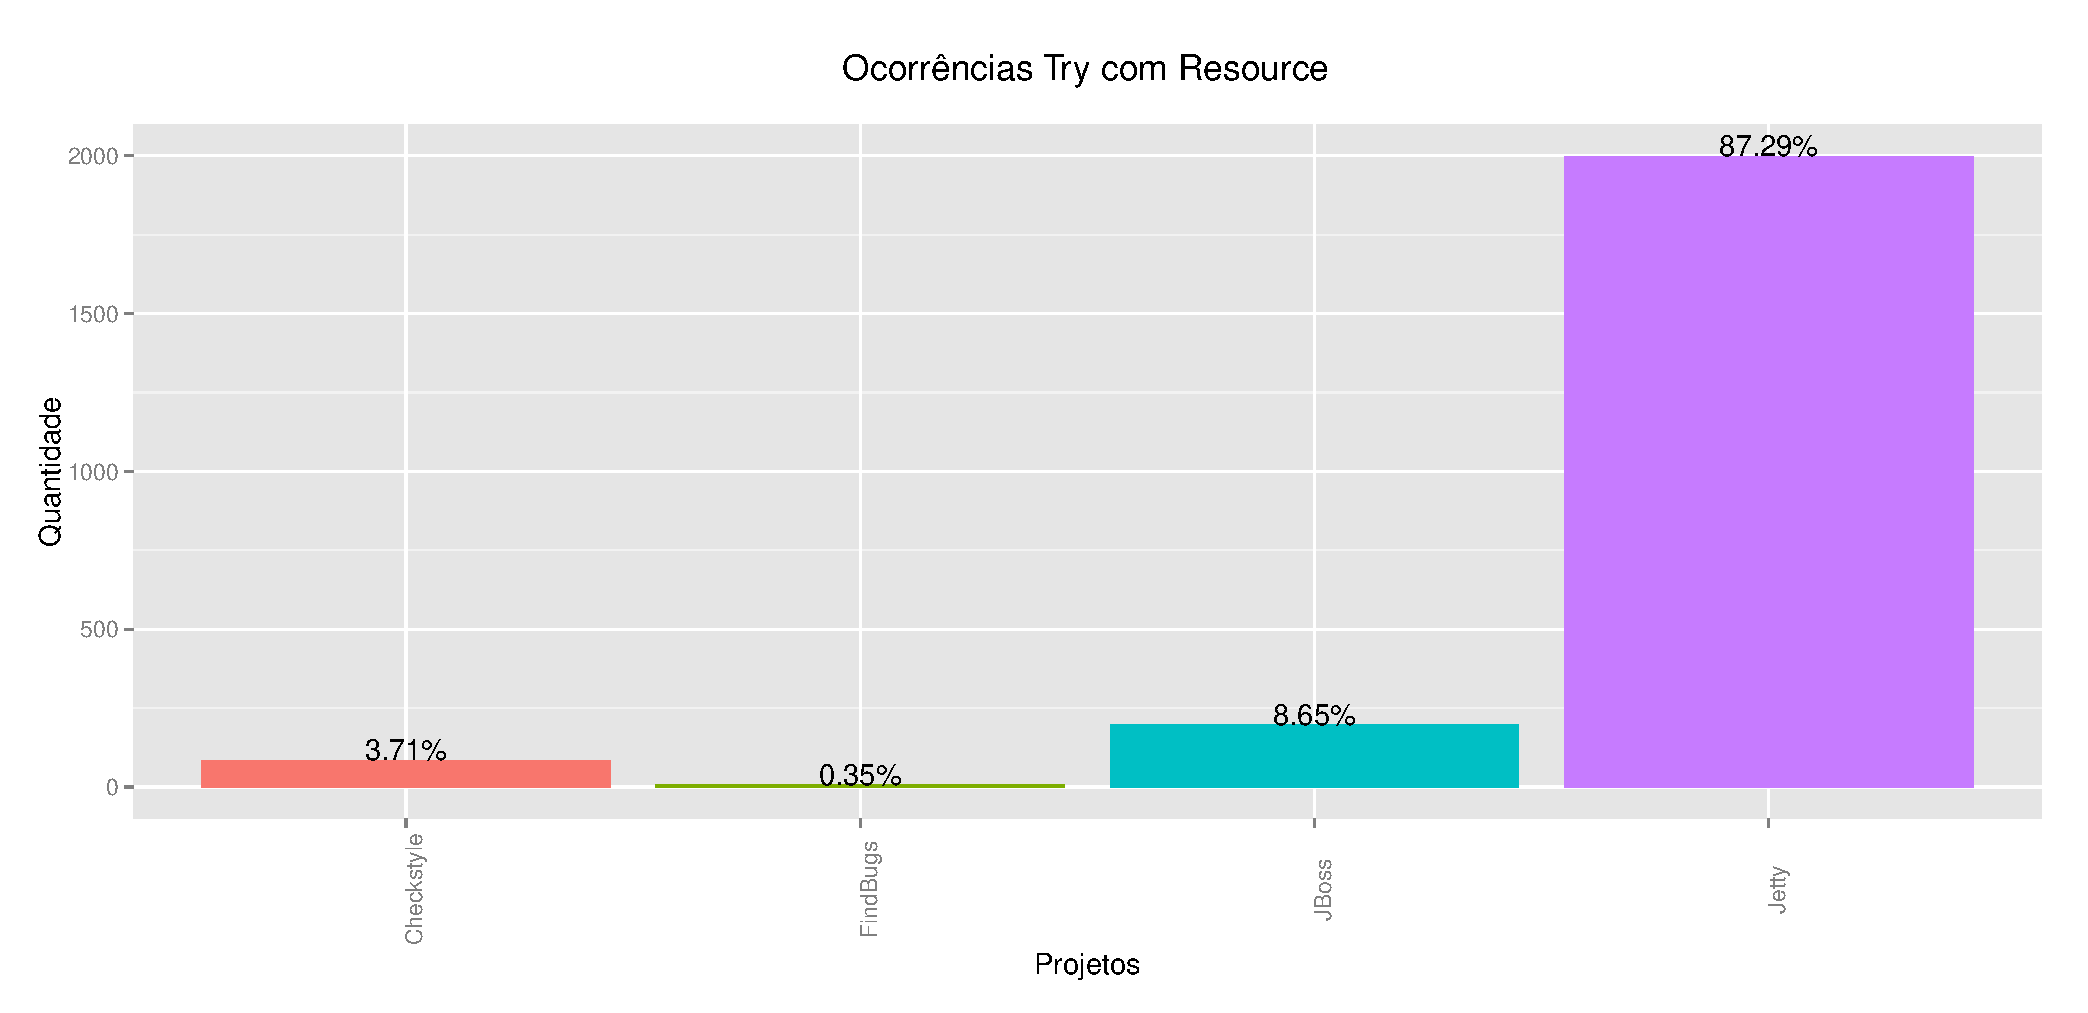
\includegraphics[scale=0.5]{Imagens/ocorrenciasTryResource}
	\label{fig:Try with Resource}
	\caption{Oportunidades de \textit{Try with Resource} nos projetos.}
\end{figure}



\section{Switch String}

  \chapter{Considerações Finais e Projeto Fututos}
Dada uma redução significativa de código duplicado no caso da adoção de \textit{multicatch} é impossível acreditar que projetos tão renomado não fazem uso desta \textit{feature}. Ignorando uma característica que prove um código mais conciso e elegante conforme a proposta original desta \textit{feature} pela Oracle em 2007. Entretanto vale ressaltar ainda como ponto vital no desenvolvimento que equipes não tem a evolução da linguagem como ponto relevante no desenvolvimento de seu produto. 
Conforme relatado pela equipe do Spring em seu forum a adoção de características como \textit{Lambda} ou \textit{Multicatch} ainda não foram adotadas pois seus projetos são desenvolvidos em Java7 e que ainda não faz total uso das \textit{features} de Java7 o que leva a crer que somente farão adesão de features de Java8 quando utilizarem totalmente Java7.

\section{Projeto Futuro}
Existe também a possibilidade da extensão do anaslisador para indentificar \textit{multicatch} por similaridade onde atualmente essa tarefa é realizada por igualdade. Com um algoritmo eficiente que detecte a similaridade com certeza a eficiência dessa \textit{feature} irá crescer consideravelmente o que acarretará em um \textit{refactoring} ainda mais significativo. Existe ainda a possibilidade de ampliar a pesquisa para encontrar objetos que contém método \textit{close} dentro de blocos \textit{Try's} o que acarretaria em um outro \textit{refactoring} visando migrar estes objetos para os \textit{resources} que estes pode receber.

Existem diversas caracterísitcas evolutivas da linguagem \textit{Java} a serem atacados tais como \textit{boilerplate} e \textit{anonymousInnerClass} que podem ser tratados com \textit{LambdaExpression}. Um projeto futuro de grande valia seria a evolução desta ferramenta para que obter um \textit{refactoring} automático de códigos ultrapassados assim possibilitando a evolulção natural de \textit{softwares} legados e \textit{opensource}.

Como exemplo destes códigos temos o caso de \textit{EnhancedFor} que iteram sobre uma \textit{Collection} o que a evolução deste abre algumas possibilidade como a facilidade de aplicar concorrência na evolução com \textit{Lambda} o que atualmente é muito complicado adicionar concorrência em um loop.

\begin{lstlisting}
//	EnhacedFor
	List<Transaction> groceryTransactions = new Arraylist<>();
	for(Transaction t: transactions){
		if(t.getType() == Transaction.GROCERY){
			groceryTransactions.add(t);
		}
	}

//	Lambda Stream
	List<Integer> transactionsIds = 
		transactions.stream().filter(t -> t.getType() == Transaction.GROCERY);
\end{lstlisting}
  
  \postextual
  \bibliographystyle{plain}
  \bibliography{referencias/referencias}
	
 % \printglossaries
\end{document}
